\documentclass[twoside]{book}

% Packages required by doxygen
\usepackage{fixltx2e}
\usepackage{calc}
\usepackage{doxygen}
\usepackage[export]{adjustbox} % also loads graphicx
\usepackage{graphicx}
\usepackage[utf8]{inputenc}
\usepackage{makeidx}
\usepackage{multicol}
\usepackage{multirow}
\PassOptionsToPackage{warn}{textcomp}
\usepackage{textcomp}
\usepackage[nointegrals]{wasysym}
\usepackage[table]{xcolor}

% Font selection
\usepackage[T1]{fontenc}
\usepackage[scaled=.90]{helvet}
\usepackage{courier}
\usepackage{amssymb}
\usepackage{sectsty}
\renewcommand{\familydefault}{\sfdefault}
\allsectionsfont{%
  \fontseries{bc}\selectfont%
  \color{darkgray}%
}
\renewcommand{\DoxyLabelFont}{%
  \fontseries{bc}\selectfont%
  \color{darkgray}%
}
\newcommand{\+}{\discretionary{\mbox{\scriptsize$\hookleftarrow$}}{}{}}

% Page & text layout
\usepackage{geometry}
\geometry{%
  a4paper,%
  top=2.5cm,%
  bottom=2.5cm,%
  left=2.5cm,%
  right=2.5cm%
}
\tolerance=750
\hfuzz=15pt
\hbadness=750
\setlength{\emergencystretch}{15pt}
\setlength{\parindent}{0cm}
\setlength{\parskip}{3ex plus 2ex minus 2ex}
\makeatletter
\renewcommand{\paragraph}{%
  \@startsection{paragraph}{4}{0ex}{-1.0ex}{1.0ex}{%
    \normalfont\normalsize\bfseries\SS@parafont%
  }%
}
\renewcommand{\subparagraph}{%
  \@startsection{subparagraph}{5}{0ex}{-1.0ex}{1.0ex}{%
    \normalfont\normalsize\bfseries\SS@subparafont%
  }%
}
\makeatother

% Headers & footers
\usepackage{fancyhdr}
\pagestyle{fancyplain}
\fancyhead[LE]{\fancyplain{}{\bfseries\thepage}}
\fancyhead[CE]{\fancyplain{}{}}
\fancyhead[RE]{\fancyplain{}{\bfseries\leftmark}}
\fancyhead[LO]{\fancyplain{}{\bfseries\rightmark}}
\fancyhead[CO]{\fancyplain{}{}}
\fancyhead[RO]{\fancyplain{}{\bfseries\thepage}}
\fancyfoot[LE]{\fancyplain{}{}}
\fancyfoot[CE]{\fancyplain{}{}}
\fancyfoot[RE]{\fancyplain{}{\bfseries\scriptsize Generated by Doxygen }}
\fancyfoot[LO]{\fancyplain{}{\bfseries\scriptsize Generated by Doxygen }}
\fancyfoot[CO]{\fancyplain{}{}}
\fancyfoot[RO]{\fancyplain{}{}}
\renewcommand{\footrulewidth}{0.4pt}
\renewcommand{\chaptermark}[1]{%
  \markboth{#1}{}%
}
\renewcommand{\sectionmark}[1]{%
  \markright{\thesection\ #1}%
}

% Indices & bibliography
\usepackage{natbib}
\usepackage[titles]{tocloft}
\setcounter{tocdepth}{3}
\setcounter{secnumdepth}{5}
\makeindex

% Hyperlinks (required, but should be loaded last)
\usepackage{ifpdf}
\ifpdf
  \usepackage[pdftex,pagebackref=true]{hyperref}
\else
  \usepackage[ps2pdf,pagebackref=true]{hyperref}
\fi
\hypersetup{%
  colorlinks=true,%
  linkcolor=blue,%
  citecolor=blue,%
  unicode%
}

% Custom commands
\newcommand{\clearemptydoublepage}{%
  \newpage{\pagestyle{empty}\cleardoublepage}%
}

\usepackage{caption}
\captionsetup{labelsep=space,justification=centering,font={bf},singlelinecheck=off,skip=4pt,position=top}

%===== C O N T E N T S =====

\begin{document}

% Titlepage & ToC
\hypersetup{pageanchor=false,
             bookmarksnumbered=true,
             pdfencoding=unicode
            }
\pagenumbering{roman}
\begin{titlepage}
\vspace*{7cm}
\begin{center}%
{\Large dg\+\_\+tools }\\
\vspace*{1cm}
{\large Generated by Doxygen 1.8.11}\\
\end{center}
\end{titlepage}
\clearemptydoublepage
\tableofcontents
\clearemptydoublepage
\pagenumbering{arabic}
\hypersetup{pageanchor=true}

%--- Begin generated contents ---
\chapter{dg\+\_\+tools}
\label{md_readme}
\hypertarget{md_readme}{}
\subsection*{What is it}

Dynamic graph \char`\"{}glue code\char`\"{} responsible for the instanciation of the graph and the python interpreter. Provide a R\+OS server in order to create distant R\+OS clients.

\subsection*{Authors}


\begin{DoxyItemize}
\item Maximilien Naveau
\item Julian Viereck
\item Andrea Delprete
\end{DoxyItemize}

\subsection*{Copyrights}

Copyright (c) 2019, New York University and Max Planck Gesellschaft.

\subsection*{License}

License B\+S\+D-\/3-\/\+Clause

\subsection*{Installation\+:}

This is a ros package so it should be in a R\+OS environment. One can still test its compilation by using the following instruction\+:

`cd \hyperlink{namespacedynamic__graph__manager}{dynamic\+\_\+graph\+\_\+manager} mkdir \+\_\+build cd \+\_\+build cmake .. make -\/j8`

\subsection*{Usage\+:}

Inherite from the class Dynamic\+Graph\+Manager and overload the three functions responsible for the hardware\+: \begin{DoxyVerb} `virtual void initialize_hardware_communication_process()`

 `virtual void get_sensors_to_map(VectorDGMap&)`
\end{DoxyVerb}


and \begin{DoxyVerb}`virtual void set_motor_controls_from_map(const VectorDGMap&)`
\end{DoxyVerb}


\subsection*{Documentation\+:}

See demo and unit tests for more information on the A\+PI. Doxygen informations are available by calling\+: \begin{DoxyVerb}`catkin_make -DBUILD_DOCUMENTATION=ON`\end{DoxyVerb}
 
\chapter{License}
\label{license}
\hypertarget{license}{}

\begin{DoxyRefList}
\item[\label{license__license000001}%
\Hypertarget{license__license000001}%
File \hyperlink{yaml__cpp__fwd_8hpp}{yaml\+\_\+cpp\+\_\+fwd.hpp} ]License B\+S\+D-\/3-\/\+Clause  
\item[\label{license__license000002}%
\Hypertarget{license__license000002}%
File \hyperlink{yaml__eigen_8h}{yaml\+\_\+eigen.h} ]License B\+S\+D-\/3-\/\+Clause  
\item[\label{license__license000003}%
\Hypertarget{license__license000003}%
File \hyperlink{yaml__tools_8hpp}{yaml\+\_\+tools.hpp} ]License B\+S\+D-\/3-\/\+Clause 
\end{DoxyRefList}
\chapter{Namespace Index}
\section{Namespace List}
Here is a list of all documented namespaces with brief descriptions\+:\begin{DoxyCompactList}
\item\contentsline{section}{\hyperlink{namespacedynamic__graph}{dynamic\+\_\+graph} \\*This is this package namespace in order to avoid naming conflict }{\pageref{namespacedynamic__graph}}{}
\item\contentsline{section}{\hyperlink{namespacedynamic__graph_1_1specific}{dynamic\+\_\+graph\+::specific} \\*Types dedicated to identify pairs of (dg,ros) data }{\pageref{namespacedynamic__graph_1_1specific}}{}
\item\contentsline{section}{\hyperlink{namespacedynamic__graph__manager}{dynamic\+\_\+graph\+\_\+manager} \\*Example of hardware communication client based on R\+OS }{\pageref{namespacedynamic__graph__manager}}{}
\item\contentsline{section}{\hyperlink{namespacedynamicgraph}{dynamicgraph} \\*Definition of the command }{\pageref{namespacedynamicgraph}}{}
\item\contentsline{section}{\hyperlink{namespacedynamicgraph_1_1command}{dynamicgraph\+::command} \\*This is this the namespace including the commands }{\pageref{namespacedynamicgraph_1_1command}}{}
\item\contentsline{section}{\hyperlink{namespacedynamicgraph_1_1command_1_1ros__state__publish}{dynamicgraph\+::command\+::ros\+\_\+state\+\_\+publish} \\*This is this a namespace including the ros state publisher command }{\pageref{namespacedynamicgraph_1_1command_1_1ros__state__publish}}{}
\end{DoxyCompactList}

\chapter{Hierarchical Index}
\section{Class Hierarchy}
This inheritance list is sorted roughly, but not completely, alphabetically\+:\begin{DoxyCompactList}
\item array\+\_\+members\begin{DoxyCompactList}
\item \contentsline{section}{shared\+\_\+memory\+:\+:array$<$ T, S\+I\+ZE $>$}{\pageref{classshared__memory_1_1array}}{}
\end{DoxyCompactList}
\item \contentsline{section}{shared\+\_\+memory\+:\+:Condition\+Variable}{\pageref{classshared__memory_1_1ConditionVariable}}{}
\item \contentsline{section}{Config}{\pageref{classConfig}}{}
\item exception\begin{DoxyCompactList}
\item \contentsline{section}{shared\+\_\+memory\+:\+:Allocation\+\_\+exception}{\pageref{classshared__memory_1_1Allocation__exception}}{}
\item \contentsline{section}{shared\+\_\+memory\+:\+:Memory\+\_\+overflow\+\_\+exception}{\pageref{classshared__memory_1_1Memory__overflow__exception}}{}
\item \contentsline{section}{shared\+\_\+memory\+:\+:Not\+\_\+consumed\+\_\+exception}{\pageref{classshared__memory_1_1Not__consumed__exception}}{}
\item \contentsline{section}{shared\+\_\+memory\+:\+:Unexpected\+\_\+map\+\_\+key$<$ Key $>$}{\pageref{classshared__memory_1_1Unexpected__map__key}}{}
\item \contentsline{section}{shared\+\_\+memory\+:\+:Unexpected\+\_\+size\+\_\+exception}{\pageref{classshared__memory_1_1Unexpected__size__exception}}{}
\end{DoxyCompactList}
\item \contentsline{section}{shared\+\_\+memory\+:\+:Exchange\+\_\+manager\+\_\+consumer$<$ Serializable, Q\+U\+E\+U\+E\+\_\+\+S\+I\+ZE $>$}{\pageref{classshared__memory_1_1Exchange__manager__consumer}}{}
\item \contentsline{section}{shared\+\_\+memory\+:\+:Exchange\+\_\+manager\+\_\+producer$<$ Serializable, Q\+U\+E\+U\+E\+\_\+\+S\+I\+ZE $>$}{\pageref{classshared__memory_1_1Exchange__manager__producer}}{}
\item \contentsline{section}{shared\+\_\+memory\+:\+:Four\+\_\+int\+\_\+values}{\pageref{classshared__memory_1_1Four__int__values}}{}
\item \contentsline{section}{shared\+\_\+memory\+:\+:Item$<$ S\+I\+ZE $>$}{\pageref{classshared__memory_1_1Item}}{}
\item \contentsline{section}{shared\+\_\+memory\+:\+:Lock}{\pageref{classshared__memory_1_1Lock}}{}
\item \contentsline{section}{shared\+\_\+memory\+:\+:Locked\+Condition\+Variable}{\pageref{classshared__memory_1_1LockedConditionVariable}}{}
\item \contentsline{section}{Measure\+Time}{\pageref{structMeasureTime}}{}
\item \contentsline{section}{shared\+\_\+memory\+:\+:Mutex}{\pageref{classshared__memory_1_1Mutex}}{}
\item \contentsline{section}{shared\+\_\+memory\+:\+:Segment\+Info}{\pageref{classshared__memory_1_1SegmentInfo}}{}
\item \contentsline{section}{Serializable$<$ S\+I\+ZE $>$}{\pageref{classSerializable}}{}
\item \contentsline{section}{shared\+\_\+memory\+:\+:Serializable\+\_\+exchange$<$ Serializable $>$}{\pageref{classshared__memory_1_1Serializable__exchange}}{}
\item \contentsline{section}{Serializable\+Example}{\pageref{classSerializableExample}}{}
\item \contentsline{section}{shared\+\_\+memory\+:\+:Serializer$<$ Serializable $>$}{\pageref{classshared__memory_1_1Serializer}}{}
\item \contentsline{section}{shared\+\_\+memory\+:\+:Shared\+Memory\+Segment}{\pageref{classshared__memory_1_1SharedMemorySegment}}{}
\item \contentsline{section}{shared\+\_\+memory\+:\+:Shm\+Type\+Helper$<$ Elem\+Type $>$}{\pageref{structshared__memory_1_1ShmTypeHelper}}{}
\end{DoxyCompactList}

\chapter{Class Index}
\section{Class List}
Here are the classes, structs, unions and interfaces with brief descriptions\+:\begin{DoxyCompactList}
\item\contentsline{section}{\hyperlink{classshared__memory_1_1Allocation__exception}{shared\+\_\+memory\+::\+Allocation\+\_\+exception} }{\pageref{classshared__memory_1_1Allocation__exception}}{}
\item\contentsline{section}{\hyperlink{classshared__memory_1_1array}{shared\+\_\+memory\+::array$<$ T, S\+I\+Z\+E $>$} \\*Implement a shared array stored on a shared memory segment }{\pageref{classshared__memory_1_1array}}{}
\item\contentsline{section}{\hyperlink{classshared__memory_1_1internal_1_1array__members}{shared\+\_\+memory\+::internal\+::array\+\_\+members$<$ T, S\+I\+Z\+E, Enable $>$} }{\pageref{classshared__memory_1_1internal_1_1array__members}}{}
\item\contentsline{section}{\hyperlink{classshared__memory_1_1internal_1_1array__members_3_01T_00_010_00_01typename_01std_1_1enable__ifb2fde5f96702510d664610c5e9570772}{shared\+\_\+memory\+::internal\+::array\+\_\+members$<$ T, 0, typename std\+::enable\+\_\+if$<$ std\+::is\+\_\+fundamental$<$ T $>$\+::value $>$\+::type $>$} }{\pageref{classshared__memory_1_1internal_1_1array__members_3_01T_00_010_00_01typename_01std_1_1enable__ifb2fde5f96702510d664610c5e9570772}}{}
\item\contentsline{section}{\hyperlink{classshared__memory_1_1internal_1_1array__members_3_01T_00_01SIZE_00_01typename_01std_1_1enable_de9984c52d14535c26d7a424fbd87fe2}{shared\+\_\+memory\+::internal\+::array\+\_\+members$<$ T, S\+I\+Z\+E, typename std\+::enable\+\_\+if$<$ std\+::is\+\_\+fundamental$<$ T $>$\+::value \&\&\+S\+I\+Z\+E!=0 $>$\+::type $>$} }{\pageref{classshared__memory_1_1internal_1_1array__members_3_01T_00_01SIZE_00_01typename_01std_1_1enable_de9984c52d14535c26d7a424fbd87fe2}}{}
\item\contentsline{section}{\hyperlink{classshared__memory_1_1ConditionVariable}{shared\+\_\+memory\+::\+Condition\+Variable} }{\pageref{classshared__memory_1_1ConditionVariable}}{}
\item\contentsline{section}{\hyperlink{classConfig}{Config} }{\pageref{classConfig}}{}
\item\contentsline{section}{\hyperlink{classshared__memory_1_1Exchange__manager__consumer}{shared\+\_\+memory\+::\+Exchange\+\_\+manager\+\_\+consumer$<$ Serializable, Q\+U\+E\+U\+E\+\_\+\+S\+I\+Z\+E $>$} }{\pageref{classshared__memory_1_1Exchange__manager__consumer}}{}
\item\contentsline{section}{\hyperlink{classshared__memory_1_1internal_1_1Exchange__manager__memory}{shared\+\_\+memory\+::internal\+::\+Exchange\+\_\+manager\+\_\+memory$<$ Serializable, Q\+U\+E\+U\+E\+\_\+\+S\+I\+Z\+E $>$} }{\pageref{classshared__memory_1_1internal_1_1Exchange__manager__memory}}{}
\item\contentsline{section}{\hyperlink{classshared__memory_1_1Exchange__manager__producer}{shared\+\_\+memory\+::\+Exchange\+\_\+manager\+\_\+producer$<$ Serializable, Q\+U\+E\+U\+E\+\_\+\+S\+I\+Z\+E $>$} }{\pageref{classshared__memory_1_1Exchange__manager__producer}}{}
\item\contentsline{section}{\hyperlink{classshared__memory_1_1Four__int__values}{shared\+\_\+memory\+::\+Four\+\_\+int\+\_\+values} \\*Example of an instance that can be serialized }{\pageref{classshared__memory_1_1Four__int__values}}{}
\item\contentsline{section}{\hyperlink{classshared__memory_1_1Item}{shared\+\_\+memory\+::\+Item$<$ S\+I\+Z\+E $>$} }{\pageref{classshared__memory_1_1Item}}{}
\item\contentsline{section}{\hyperlink{classshared__memory_1_1Lock}{shared\+\_\+memory\+::\+Lock} \\*A scope lock object for locking a shared memory mutex, to use for example with a shared memory condition variable }{\pageref{classshared__memory_1_1Lock}}{}
\item\contentsline{section}{\hyperlink{classshared__memory_1_1LockedConditionVariable}{shared\+\_\+memory\+::\+Locked\+Condition\+Variable} \\*Here as a anonymous layer on top of the boost intersprocess condition variable labrary }{\pageref{classshared__memory_1_1LockedConditionVariable}}{}
\item\contentsline{section}{\hyperlink{structMeasureTime}{Measure\+Time} }{\pageref{structMeasureTime}}{}
\item\contentsline{section}{\hyperlink{classshared__memory_1_1Memory__overflow__exception}{shared\+\_\+memory\+::\+Memory\+\_\+overflow\+\_\+exception} }{\pageref{classshared__memory_1_1Memory__overflow__exception}}{}
\item\contentsline{section}{\hyperlink{classshared__memory_1_1Mutex}{shared\+\_\+memory\+::\+Mutex} }{\pageref{classshared__memory_1_1Mutex}}{}
\item\contentsline{section}{\hyperlink{classshared__memory_1_1Not__consumed__exception}{shared\+\_\+memory\+::\+Not\+\_\+consumed\+\_\+exception} }{\pageref{classshared__memory_1_1Not__consumed__exception}}{}
\item\contentsline{section}{\hyperlink{classshared__memory_1_1SegmentInfo}{shared\+\_\+memory\+::\+Segment\+Info} \\*Encapsulate information related to a shared memory segment }{\pageref{classshared__memory_1_1SegmentInfo}}{}
\item\contentsline{section}{\hyperlink{classSerializable}{Serializable$<$ S\+I\+Z\+E $>$} }{\pageref{classSerializable}}{}
\item\contentsline{section}{\hyperlink{classshared__memory_1_1Serializable__exchange}{shared\+\_\+memory\+::\+Serializable\+\_\+exchange$<$ Serializable $>$} }{\pageref{classshared__memory_1_1Serializable__exchange}}{}
\item\contentsline{section}{\hyperlink{classSerializableExample}{Serializable\+Example} }{\pageref{classSerializableExample}}{}
\item\contentsline{section}{\hyperlink{classshared__memory_1_1internal_1_1Serialized__read}{shared\+\_\+memory\+::internal\+::\+Serialized\+\_\+read$<$ Serializable $>$} }{\pageref{classshared__memory_1_1internal_1_1Serialized__read}}{}
\item\contentsline{section}{\hyperlink{classshared__memory_1_1internal_1_1Serialized__write}{shared\+\_\+memory\+::internal\+::\+Serialized\+\_\+write$<$ Serializable $>$} }{\pageref{classshared__memory_1_1internal_1_1Serialized__write}}{}
\item\contentsline{section}{\hyperlink{classshared__memory_1_1Serializer}{shared\+\_\+memory\+::\+Serializer$<$ Serializable $>$} }{\pageref{classshared__memory_1_1Serializer}}{}
\item\contentsline{section}{\hyperlink{classshared__memory_1_1SharedMemorySegment}{shared\+\_\+memory\+::\+Shared\+Memory\+Segment} \\*The \hyperlink{classshared__memory_1_1SharedMemorySegment}{Shared\+Memory\+Segment} contains the pointers of the shared objects in on shared memrory segment }{\pageref{classshared__memory_1_1SharedMemorySegment}}{}
\item\contentsline{section}{\hyperlink{structshared__memory_1_1ShmTypeHelper}{shared\+\_\+memory\+::\+Shm\+Type\+Helper$<$ Elem\+Type $>$} \\*\hyperlink{structshared__memory_1_1ShmTypeHelper}{Shm\+Type\+Helper} is a small struct that allow the definition of templated typedef }{\pageref{structshared__memory_1_1ShmTypeHelper}}{}
\item\contentsline{section}{\hyperlink{classshared__memory_1_1Unexpected__map__key}{shared\+\_\+memory\+::\+Unexpected\+\_\+map\+\_\+key$<$ Key $>$} }{\pageref{classshared__memory_1_1Unexpected__map__key}}{}
\item\contentsline{section}{\hyperlink{classshared__memory_1_1Unexpected__size__exception}{shared\+\_\+memory\+::\+Unexpected\+\_\+size\+\_\+exception} }{\pageref{classshared__memory_1_1Unexpected__size__exception}}{}
\end{DoxyCompactList}

\chapter{File Index}
\section{File List}
Here is a list of all documented files with brief descriptions\+:\begin{DoxyCompactList}
\item\contentsline{section}{include/dg\+\_\+blmc\+\_\+robots/\hyperlink{common__header_8hpp}{common\+\_\+header.\+hpp} }{\pageref{common__header_8hpp}}{}
\item\contentsline{section}{include/dg\+\_\+blmc\+\_\+robots/\hyperlink{dgm__single__motor_8hpp}{dgm\+\_\+single\+\_\+motor.\+hpp} }{\pageref{dgm__single__motor_8hpp}}{}
\item\contentsline{section}{include/dg\+\_\+blmc\+\_\+robots/{\bfseries dgm\+\_\+solo12.\+hpp} }{\pageref{dgm__solo12_8hpp}}{}
\item\contentsline{section}{include/dg\+\_\+blmc\+\_\+robots/{\bfseries dgm\+\_\+solo8.\+hpp} }{\pageref{dgm__solo8_8hpp}}{}
\item\contentsline{section}{include/dg\+\_\+blmc\+\_\+robots/{\bfseries dgm\+\_\+solo8ti.\+hpp} }{\pageref{dgm__solo8ti_8hpp}}{}
\item\contentsline{section}{include/dg\+\_\+blmc\+\_\+robots/{\bfseries dgm\+\_\+solo\+\_\+simple\+\_\+simu.\+hpp} }{\pageref{dgm__solo__simple__simu_8hpp}}{}
\item\contentsline{section}{include/dg\+\_\+blmc\+\_\+robots/\hyperlink{dgm__stuggihop_8hpp}{dgm\+\_\+stuggihop.\+hpp} }{\pageref{dgm__stuggihop_8hpp}}{}
\item\contentsline{section}{include/dg\+\_\+blmc\+\_\+robots/{\bfseries dgm\+\_\+teststand.\+hpp} }{\pageref{dgm__teststand_8hpp}}{}
\item\contentsline{section}{src/\hyperlink{dgm__solo__simple__simu_8cpp}{dgm\+\_\+solo\+\_\+simple\+\_\+simu.\+cpp} \\*The hardware wrapper of the solo naive simulation }{\pageref{dgm__solo__simple__simu_8cpp}}{}
\item\contentsline{section}{src/\hyperlink{dgm__stuggihop_8cpp}{dgm\+\_\+stuggihop.\+cpp} \\*D\+GM wrapper around the stuggihop robot }{\pageref{dgm__stuggihop_8cpp}}{}
\end{DoxyCompactList}

\chapter{Namespace Documentation}
\hypertarget{namespacepy__dg__tools}{}\section{py\+\_\+dg\+\_\+tools Namespace Reference}
\label{namespacepy__dg__tools}\index{py\+\_\+dg\+\_\+tools@{py\+\_\+dg\+\_\+tools}}


Generate trajectories in python using scypy.  




\subsection{Detailed Description}
Generate trajectories in python using scypy. 

This script converts data dumps from dynamic graph to a R\+AI compatible npz format.

Contains functions that help the use of sot-\/core.

Contains generic impedance control functions that will be used by the impedance\+\_\+controller.

\begin{DoxyAuthor}{Author}
Avadesh Meduri 
\end{DoxyAuthor}
\begin{DoxyRefDesc}{License}
\item[\hyperlink{license__license000011}{License}]License B\+S\+D-\/3-\/\+Clause \end{DoxyRefDesc}
\begin{DoxyCopyright}{Copyright}
Copyright (c) 2019, New York University and Max Planck Gesellschaft. 
\end{DoxyCopyright}
\begin{DoxyDate}{Date}
2019-\/05-\/22
\end{DoxyDate}
\begin{DoxyAuthor}{Author}
Maximilien Naveau 
\end{DoxyAuthor}
\begin{DoxyRefDesc}{License}
\item[\hyperlink{license__license000012}{License}]License B\+S\+D-\/3-\/\+Clause \end{DoxyRefDesc}
\begin{DoxyCopyright}{Copyright}
Copyright (c) 2019, New York University and Max Planck Gesellschaft. 
\end{DoxyCopyright}
\begin{DoxyDate}{Date}
2019-\/08-\/01
\end{DoxyDate}
\begin{DoxyAuthor}{Author}
Avadesh Meduri 
\end{DoxyAuthor}
\begin{DoxyRefDesc}{License}
\item[\hyperlink{license__license000016}{License}]License B\+S\+D-\/3-\/\+Clause \end{DoxyRefDesc}
\begin{DoxyCopyright}{Copyright}
Copyright (c) 2019, New York University and Max Planck Gesellschaft. 
\end{DoxyCopyright}
\begin{DoxyDate}{Date}
2019-\/03-\/01
\end{DoxyDate}
\begin{DoxyAuthor}{Author}
Avadesh Meduri 
\end{DoxyAuthor}
\begin{DoxyRefDesc}{License}
\item[\hyperlink{license__license000019}{License}]License B\+S\+D-\/3-\/\+Clause \end{DoxyRefDesc}
\begin{DoxyCopyright}{Copyright}
Copyright (c) 2019, New York University and Max Planck Gesellschaft. 
\end{DoxyCopyright}
\begin{DoxyDate}{Date}
2019-\/03-\/01
\end{DoxyDate}
\begin{DoxyAuthor}{Author}
Julian Viereck 
\end{DoxyAuthor}
\begin{DoxyRefDesc}{License}
\item[\hyperlink{license__license000020}{License}]License B\+S\+D-\/3-\/\+Clause \end{DoxyRefDesc}
\begin{DoxyCopyright}{Copyright}
Copyright (c) 2019, New York University and Max Planck Gesellschaft. 
\end{DoxyCopyright}
\begin{DoxyDate}{Date}
2018-\/12-\/13 
\end{DoxyDate}

\chapter{Class Documentation}
\hypertarget{classpython_1_1dg__tools_1_1math__small__entities_1_1Add2Vectors}{}\section{python.\+dg\+\_\+tools.\+math\+\_\+small\+\_\+entities.\+Add2\+Vectors Class Reference}
\label{classpython_1_1dg__tools_1_1math__small__entities_1_1Add2Vectors}\index{python.\+dg\+\_\+tools.\+math\+\_\+small\+\_\+entities.\+Add2\+Vectors@{python.\+dg\+\_\+tools.\+math\+\_\+small\+\_\+entities.\+Add2\+Vectors}}


interface to the Add\+\_\+of\+\_\+vector entity  




Inheritance diagram for python.\+dg\+\_\+tools.\+math\+\_\+small\+\_\+entities.\+Add2\+Vectors\+:
\nopagebreak
\begin{figure}[H]
\begin{center}
\leavevmode
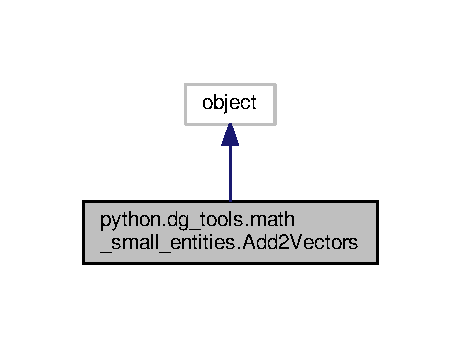
\includegraphics[width=221pt]{classpython_1_1dg__tools_1_1math__small__entities_1_1Add2Vectors__inherit__graph}
\end{center}
\end{figure}


Collaboration diagram for python.\+dg\+\_\+tools.\+math\+\_\+small\+\_\+entities.\+Add2\+Vectors\+:
\nopagebreak
\begin{figure}[H]
\begin{center}
\leavevmode
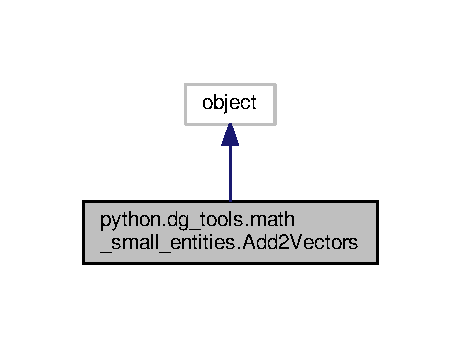
\includegraphics[width=221pt]{classpython_1_1dg__tools_1_1math__small__entities_1_1Add2Vectors__coll__graph}
\end{center}
\end{figure}
\subsection*{Public Member Functions}
\begin{DoxyCompactItemize}
\item 
def {\bfseries \+\_\+\+\_\+init\+\_\+\+\_\+} (self, vector\+\_\+sin1, vector\+\_\+sin2, entity\+\_\+name=\textquotesingle{}\textquotesingle{})\hypertarget{classpython_1_1dg__tools_1_1math__small__entities_1_1Add2Vectors_aac46b1275aae7510126012c38e6ba6dc}{}\label{classpython_1_1dg__tools_1_1math__small__entities_1_1Add2Vectors_aac46b1275aae7510126012c38e6ba6dc}

\end{DoxyCompactItemize}
\subsection*{Public Attributes}
\begin{DoxyCompactItemize}
\item 
{\bfseries op}\hypertarget{classpython_1_1dg__tools_1_1math__small__entities_1_1Add2Vectors_a05f25ea034d56ca14cd8c83414d9fd6e}{}\label{classpython_1_1dg__tools_1_1math__small__entities_1_1Add2Vectors_a05f25ea034d56ca14cd8c83414d9fd6e}

\item 
{\bfseries sin1}\hypertarget{classpython_1_1dg__tools_1_1math__small__entities_1_1Add2Vectors_a83e5c3083168c62acf3d93802b396b76}{}\label{classpython_1_1dg__tools_1_1math__small__entities_1_1Add2Vectors_a83e5c3083168c62acf3d93802b396b76}

\item 
{\bfseries sin2}\hypertarget{classpython_1_1dg__tools_1_1math__small__entities_1_1Add2Vectors_a41be9171214f0243162899da628c1a6d}{}\label{classpython_1_1dg__tools_1_1math__small__entities_1_1Add2Vectors_a41be9171214f0243162899da628c1a6d}

\item 
{\bfseries sout}\hypertarget{classpython_1_1dg__tools_1_1math__small__entities_1_1Add2Vectors_ae865de9c7a4c7d2e03b8c685326e0b1f}{}\label{classpython_1_1dg__tools_1_1math__small__entities_1_1Add2Vectors_ae865de9c7a4c7d2e03b8c685326e0b1f}

\end{DoxyCompactItemize}


\subsection{Detailed Description}
interface to the Add\+\_\+of\+\_\+vector entity 

The documentation for this class was generated from the following file\+:\begin{DoxyCompactItemize}
\item 
python/dg\+\_\+tools/math\+\_\+small\+\_\+entities.\+py\end{DoxyCompactItemize}

\hypertarget{classpython_1_1dg__tools_1_1utils_1_1BaseOperatorSignal}{}\section{python.\+dg\+\_\+tools.\+utils.\+Base\+Operator\+Signal Class Reference}
\label{classpython_1_1dg__tools_1_1utils_1_1BaseOperatorSignal}\index{python.\+dg\+\_\+tools.\+utils.\+Base\+Operator\+Signal@{python.\+dg\+\_\+tools.\+utils.\+Base\+Operator\+Signal}}


Inheritance diagram for python.\+dg\+\_\+tools.\+utils.\+Base\+Operator\+Signal\+:
\nopagebreak
\begin{figure}[H]
\begin{center}
\leavevmode
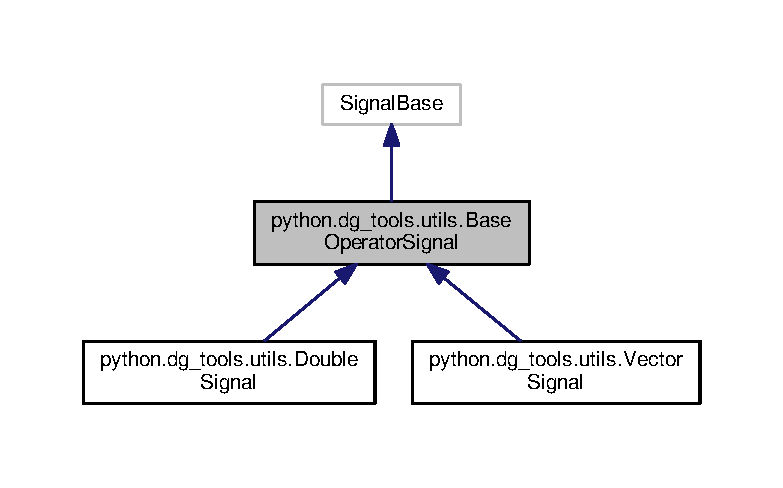
\includegraphics[width=350pt]{classpython_1_1dg__tools_1_1utils_1_1BaseOperatorSignal__inherit__graph}
\end{center}
\end{figure}


Collaboration diagram for python.\+dg\+\_\+tools.\+utils.\+Base\+Operator\+Signal\+:
\nopagebreak
\begin{figure}[H]
\begin{center}
\leavevmode
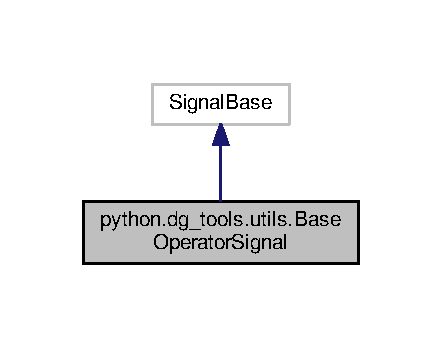
\includegraphics[width=212pt]{classpython_1_1dg__tools_1_1utils_1_1BaseOperatorSignal__coll__graph}
\end{center}
\end{figure}
\subsection*{Public Member Functions}
\begin{DoxyCompactItemize}
\item 
def {\bfseries \+\_\+\+\_\+init\+\_\+\+\_\+} (self, sig)\hypertarget{classpython_1_1dg__tools_1_1utils_1_1BaseOperatorSignal_a675957cd6f20ee47e246e6d08b7e2641}{}\label{classpython_1_1dg__tools_1_1utils_1_1BaseOperatorSignal_a675957cd6f20ee47e246e6d08b7e2641}

\item 
def {\bfseries name\+\_\+entity} (self, entity\+\_\+name)\hypertarget{classpython_1_1dg__tools_1_1utils_1_1BaseOperatorSignal_a8cf93a192762faa90c33c328eeef535d}{}\label{classpython_1_1dg__tools_1_1utils_1_1BaseOperatorSignal_a8cf93a192762faa90c33c328eeef535d}

\item 
def {\bfseries \+\_\+\+\_\+add\+\_\+\+\_\+} (self, other)\hypertarget{classpython_1_1dg__tools_1_1utils_1_1BaseOperatorSignal_a6a54bf43b66c1963b32da36f3525f318}{}\label{classpython_1_1dg__tools_1_1utils_1_1BaseOperatorSignal_a6a54bf43b66c1963b32da36f3525f318}

\item 
def {\bfseries \+\_\+\+\_\+mul\+\_\+\+\_\+} (self, other)\hypertarget{classpython_1_1dg__tools_1_1utils_1_1BaseOperatorSignal_a9d04a27ec48a61da338a7032545562e0}{}\label{classpython_1_1dg__tools_1_1utils_1_1BaseOperatorSignal_a9d04a27ec48a61da338a7032545562e0}

\item 
def {\bfseries \+\_\+\+\_\+sub\+\_\+\+\_\+} (self, other)\hypertarget{classpython_1_1dg__tools_1_1utils_1_1BaseOperatorSignal_a2a194afafc479a75f6e1e317bfda2f12}{}\label{classpython_1_1dg__tools_1_1utils_1_1BaseOperatorSignal_a2a194afafc479a75f6e1e317bfda2f12}

\item 
def {\bfseries \+\_\+\+\_\+div\+\_\+\+\_\+} (self, other)\hypertarget{classpython_1_1dg__tools_1_1utils_1_1BaseOperatorSignal_a6fa71ff269dd1c2d615d2e7431aac49f}{}\label{classpython_1_1dg__tools_1_1utils_1_1BaseOperatorSignal_a6fa71ff269dd1c2d615d2e7431aac49f}

\item 
def {\bfseries \+\_\+\+\_\+truediv\+\_\+\+\_\+} (self, other)\hypertarget{classpython_1_1dg__tools_1_1utils_1_1BaseOperatorSignal_a1e01d6d9c78373324d512f7d10b990b3}{}\label{classpython_1_1dg__tools_1_1utils_1_1BaseOperatorSignal_a1e01d6d9c78373324d512f7d10b990b3}

\item 
def {\bfseries \+\_\+\+\_\+repr\+\_\+\+\_\+} (self)\hypertarget{classpython_1_1dg__tools_1_1utils_1_1BaseOperatorSignal_ab444d02676387f3f15c36e101e4afdbb}{}\label{classpython_1_1dg__tools_1_1utils_1_1BaseOperatorSignal_ab444d02676387f3f15c36e101e4afdbb}

\end{DoxyCompactItemize}
\subsection*{Private Member Functions}
\begin{DoxyCompactItemize}
\item 
def {\bfseries \+\_\+op} (self, other, op\+\_\+name, op\+\_\+maps)\hypertarget{classpython_1_1dg__tools_1_1utils_1_1BaseOperatorSignal_a73302dff859ab49d1635a98f3ce28f53}{}\label{classpython_1_1dg__tools_1_1utils_1_1BaseOperatorSignal_a73302dff859ab49d1635a98f3ce28f53}

\item 
def {\bfseries \+\_\+identity} (self, entity\+\_\+name)\hypertarget{classpython_1_1dg__tools_1_1utils_1_1BaseOperatorSignal_a21ebc77be0448e1636f185dc4142a0bf}{}\label{classpython_1_1dg__tools_1_1utils_1_1BaseOperatorSignal_a21ebc77be0448e1636f185dc4142a0bf}

\end{DoxyCompactItemize}


The documentation for this class was generated from the following file\+:\begin{DoxyCompactItemize}
\item 
python/dg\+\_\+tools/utils.\+py\end{DoxyCompactItemize}

\hypertarget{classpython_1_1dg__tools_1_1filter_1_1ButterWorthFilter}{}\section{python.\+dg\+\_\+tools.\+filter.\+Butter\+Worth\+Filter Class Reference}
\label{classpython_1_1dg__tools_1_1filter_1_1ButterWorthFilter}\index{python.\+dg\+\_\+tools.\+filter.\+Butter\+Worth\+Filter@{python.\+dg\+\_\+tools.\+filter.\+Butter\+Worth\+Filter}}


Butterworth filter implementation in dynamic graph.  




Inheritance diagram for python.\+dg\+\_\+tools.\+filter.\+Butter\+Worth\+Filter\+:
\nopagebreak
\begin{figure}[H]
\begin{center}
\leavevmode
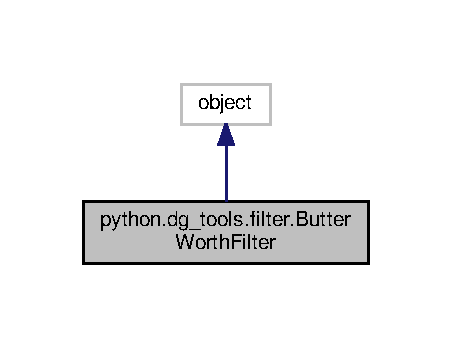
\includegraphics[width=217pt]{classpython_1_1dg__tools_1_1filter_1_1ButterWorthFilter__inherit__graph}
\end{center}
\end{figure}


Collaboration diagram for python.\+dg\+\_\+tools.\+filter.\+Butter\+Worth\+Filter\+:
\nopagebreak
\begin{figure}[H]
\begin{center}
\leavevmode
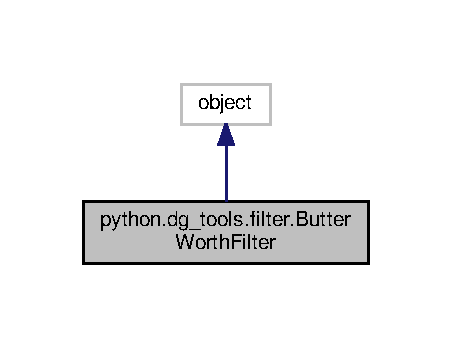
\includegraphics[width=217pt]{classpython_1_1dg__tools_1_1filter_1_1ButterWorthFilter__coll__graph}
\end{center}
\end{figure}
\subsection*{Public Member Functions}
\begin{DoxyCompactItemize}
\item 
def \hyperlink{classpython_1_1dg__tools_1_1filter_1_1ButterWorthFilter_ac9534f4a0ab7b60766183e3351093054}{\+\_\+\+\_\+init\+\_\+\+\_\+} (self, name=\char`\"{}\char`\"{})
\begin{DoxyCompactList}\small\item\em Constructor. \end{DoxyCompactList}\item 
def \hyperlink{classpython_1_1dg__tools_1_1filter_1_1ButterWorthFilter_a483e952c69af10e7c4c5d4b776c92c29}{init} (self, size\+\_\+of\+\_\+input, control\+\_\+time\+\_\+step, percentage\+\_\+nyquist\+\_\+cutoff, filter\+\_\+order)
\begin{DoxyCompactList}\small\item\em Initialize the filter using scipy. \end{DoxyCompactList}\item 
def {\bfseries update} (self, percentage\+\_\+nyquist\+\_\+cutoff, filter\+\_\+order=None)\hypertarget{classpython_1_1dg__tools_1_1filter_1_1ButterWorthFilter_ab103d1b24b289d2236ca0be5f601f7bc}{}\label{classpython_1_1dg__tools_1_1filter_1_1ButterWorthFilter_ab103d1b24b289d2236ca0be5f601f7bc}

\end{DoxyCompactItemize}
\subsection*{Public Attributes}
\begin{DoxyCompactItemize}
\item 
{\bfseries name}\hypertarget{classpython_1_1dg__tools_1_1filter_1_1ButterWorthFilter_a3c84edcefe0f321c7f24a5169d95bc86}{}\label{classpython_1_1dg__tools_1_1filter_1_1ButterWorthFilter_a3c84edcefe0f321c7f24a5169d95bc86}

\item 
\hyperlink{classpython_1_1dg__tools_1_1filter_1_1ButterWorthFilter_aaa37fb9c14becc324528c1a5eb7a0a86}{filter}
\begin{DoxyCompactList}\small\item\em Dynamic graph entity implementing an infinite impedance filter. \end{DoxyCompactList}\item 
{\bfseries sin}\hypertarget{classpython_1_1dg__tools_1_1filter_1_1ButterWorthFilter_a752671c3f15b39de6adf9cc0b3d44b33}{}\label{classpython_1_1dg__tools_1_1filter_1_1ButterWorthFilter_a752671c3f15b39de6adf9cc0b3d44b33}

\item 
{\bfseries sout}\hypertarget{classpython_1_1dg__tools_1_1filter_1_1ButterWorthFilter_ad658ec88660f576c1883ebd797112c47}{}\label{classpython_1_1dg__tools_1_1filter_1_1ButterWorthFilter_ad658ec88660f576c1883ebd797112c47}

\item 
{\bfseries size\+\_\+of\+\_\+input}\hypertarget{classpython_1_1dg__tools_1_1filter_1_1ButterWorthFilter_aac00507043d3d42798c2d9cd82fc48c9}{}\label{classpython_1_1dg__tools_1_1filter_1_1ButterWorthFilter_aac00507043d3d42798c2d9cd82fc48c9}

\item 
{\bfseries control\+\_\+time\+\_\+step}\hypertarget{classpython_1_1dg__tools_1_1filter_1_1ButterWorthFilter_a43f66675fb652ea597949603ffe6036f}{}\label{classpython_1_1dg__tools_1_1filter_1_1ButterWorthFilter_a43f66675fb652ea597949603ffe6036f}

\item 
{\bfseries percentage\+\_\+nyquist\+\_\+cutoff}\hypertarget{classpython_1_1dg__tools_1_1filter_1_1ButterWorthFilter_a678f80fb063d8985ebe597ef92965a59}{}\label{classpython_1_1dg__tools_1_1filter_1_1ButterWorthFilter_a678f80fb063d8985ebe597ef92965a59}

\item 
{\bfseries filter\+\_\+order}\hypertarget{classpython_1_1dg__tools_1_1filter_1_1ButterWorthFilter_afcf4eb37f5e300fbb14fa9094c5f36a4}{}\label{classpython_1_1dg__tools_1_1filter_1_1ButterWorthFilter_afcf4eb37f5e300fbb14fa9094c5f36a4}

\item 
{\bfseries numerator}\hypertarget{classpython_1_1dg__tools_1_1filter_1_1ButterWorthFilter_a5f449de18a557278442635e429d461a5}{}\label{classpython_1_1dg__tools_1_1filter_1_1ButterWorthFilter_a5f449de18a557278442635e429d461a5}

\item 
{\bfseries denominator}\hypertarget{classpython_1_1dg__tools_1_1filter_1_1ButterWorthFilter_a6265fc8d2dd3a429f716f6a1035cbffd}{}\label{classpython_1_1dg__tools_1_1filter_1_1ButterWorthFilter_a6265fc8d2dd3a429f716f6a1035cbffd}

\end{DoxyCompactItemize}
\subsection*{Private Member Functions}
\begin{DoxyCompactItemize}
\item 
def {\bfseries \+\_\+compute\+\_\+numerator\+\_\+denominator} (self)\hypertarget{classpython_1_1dg__tools_1_1filter_1_1ButterWorthFilter_ab35229fee7049c1b92444bab8783d62a}{}\label{classpython_1_1dg__tools_1_1filter_1_1ButterWorthFilter_ab35229fee7049c1b92444bab8783d62a}

\end{DoxyCompactItemize}


\subsection{Detailed Description}
Butterworth filter implementation in dynamic graph. 

Computes the Butterworth filter coefficient using scipy and create the appropriate dynamic graph filter. 

\subsection{Constructor \& Destructor Documentation}
\index{python\+::dg\+\_\+tools\+::filter\+::\+Butter\+Worth\+Filter@{python\+::dg\+\_\+tools\+::filter\+::\+Butter\+Worth\+Filter}!\+\_\+\+\_\+init\+\_\+\+\_\+@{\+\_\+\+\_\+init\+\_\+\+\_\+}}
\index{\+\_\+\+\_\+init\+\_\+\+\_\+@{\+\_\+\+\_\+init\+\_\+\+\_\+}!python\+::dg\+\_\+tools\+::filter\+::\+Butter\+Worth\+Filter@{python\+::dg\+\_\+tools\+::filter\+::\+Butter\+Worth\+Filter}}
\subsubsection[{\texorpdfstring{\+\_\+\+\_\+init\+\_\+\+\_\+(self, name="""")}{__init__(self, name="")}}]{\setlength{\rightskip}{0pt plus 5cm}def python.\+dg\+\_\+tools.\+filter.\+Butter\+Worth\+Filter.\+\_\+\+\_\+init\+\_\+\+\_\+ (
\begin{DoxyParamCaption}
\item[{}]{self, }
\item[{}]{name = {\ttfamily \char`\"{}\char`\"{}}}
\end{DoxyParamCaption}
)}\hypertarget{classpython_1_1dg__tools_1_1filter_1_1ButterWorthFilter_ac9534f4a0ab7b60766183e3351093054}{}\label{classpython_1_1dg__tools_1_1filter_1_1ButterWorthFilter_ac9534f4a0ab7b60766183e3351093054}


Constructor. 

name\+: 

\subsection{Member Function Documentation}
\index{python\+::dg\+\_\+tools\+::filter\+::\+Butter\+Worth\+Filter@{python\+::dg\+\_\+tools\+::filter\+::\+Butter\+Worth\+Filter}!init@{init}}
\index{init@{init}!python\+::dg\+\_\+tools\+::filter\+::\+Butter\+Worth\+Filter@{python\+::dg\+\_\+tools\+::filter\+::\+Butter\+Worth\+Filter}}
\subsubsection[{\texorpdfstring{init(self, size\+\_\+of\+\_\+input, control\+\_\+time\+\_\+step, percentage\+\_\+nyquist\+\_\+cutoff, filter\+\_\+order)}{init(self, size_of_input, control_time_step, percentage_nyquist_cutoff, filter_order)}}]{\setlength{\rightskip}{0pt plus 5cm}def python.\+dg\+\_\+tools.\+filter.\+Butter\+Worth\+Filter.\+init (
\begin{DoxyParamCaption}
\item[{}]{self, }
\item[{}]{size\+\_\+of\+\_\+input, }
\item[{}]{control\+\_\+time\+\_\+step, }
\item[{}]{percentage\+\_\+nyquist\+\_\+cutoff, }
\item[{}]{filter\+\_\+order}
\end{DoxyParamCaption}
)}\hypertarget{classpython_1_1dg__tools_1_1filter_1_1ButterWorthFilter_a483e952c69af10e7c4c5d4b776c92c29}{}\label{classpython_1_1dg__tools_1_1filter_1_1ButterWorthFilter_a483e952c69af10e7c4c5d4b776c92c29}


Initialize the filter using scipy. 

size\+\_\+of\+\_\+input\+: control\+\_\+time\+\_\+step\+: 
\begin{DoxyParams}{Parameters}
{\em percentage\+\_\+nyquist\+\_\+cutoff} & Range of (0., 1.) filter\+\_\+order\+: prefix\+: \\
\hline
\end{DoxyParams}


\subsection{Member Data Documentation}
\index{python\+::dg\+\_\+tools\+::filter\+::\+Butter\+Worth\+Filter@{python\+::dg\+\_\+tools\+::filter\+::\+Butter\+Worth\+Filter}!filter@{filter}}
\index{filter@{filter}!python\+::dg\+\_\+tools\+::filter\+::\+Butter\+Worth\+Filter@{python\+::dg\+\_\+tools\+::filter\+::\+Butter\+Worth\+Filter}}
\subsubsection[{\texorpdfstring{filter}{filter}}]{\setlength{\rightskip}{0pt plus 5cm}python.\+dg\+\_\+tools.\+filter.\+Butter\+Worth\+Filter.\+filter}\hypertarget{classpython_1_1dg__tools_1_1filter_1_1ButterWorthFilter_aaa37fb9c14becc324528c1a5eb7a0a86}{}\label{classpython_1_1dg__tools_1_1filter_1_1ButterWorthFilter_aaa37fb9c14becc324528c1a5eb7a0a86}


Dynamic graph entity implementing an infinite impedance filter. 



The documentation for this class was generated from the following file\+:\begin{DoxyCompactItemize}
\item 
python/dg\+\_\+tools/\hyperlink{filter_8py}{filter.\+py}\end{DoxyCompactItemize}

\hypertarget{classdynamicgraph_1_1sot_1_1Calibrator}{}\section{dynamicgraph\+:\+:sot\+:\+:Calibrator Class Reference}
\label{classdynamicgraph_1_1sot_1_1Calibrator}\index{dynamicgraph\+::sot\+::\+Calibrator@{dynamicgraph\+::sot\+::\+Calibrator}}


Inheritance diagram for dynamicgraph\+:\+:sot\+:\+:Calibrator\+:
\nopagebreak
\begin{figure}[H]
\begin{center}
\leavevmode
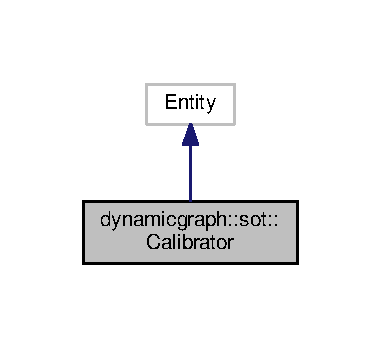
\includegraphics[width=183pt]{classdynamicgraph_1_1sot_1_1Calibrator__inherit__graph}
\end{center}
\end{figure}


Collaboration diagram for dynamicgraph\+:\+:sot\+:\+:Calibrator\+:
\nopagebreak
\begin{figure}[H]
\begin{center}
\leavevmode
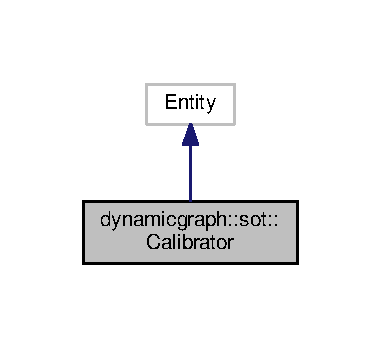
\includegraphics[width=183pt]{classdynamicgraph_1_1sot_1_1Calibrator__coll__graph}
\end{center}
\end{figure}
\subsection*{Public Member Functions}
\begin{DoxyCompactItemize}
\item 
{\bfseries Calibrator} (const std\+::string \&name)\hypertarget{classdynamicgraph_1_1sot_1_1Calibrator_ab2b86fbd9baf92285ea9147c2157a614}{}\label{classdynamicgraph_1_1sot_1_1Calibrator_ab2b86fbd9baf92285ea9147c2157a614}

\item 
virtual void {\bfseries display} (std\+::ostream \&os) const \hypertarget{classdynamicgraph_1_1sot_1_1Calibrator_ad0ab88517b0d3fe66cc65eb44d604baf}{}\label{classdynamicgraph_1_1sot_1_1Calibrator_ad0ab88517b0d3fe66cc65eb44d604baf}

\item 
virtual const std\+::string \& {\bfseries get\+Class\+Name} (void) const \hypertarget{classdynamicgraph_1_1sot_1_1Calibrator_a43555b52b4bcf1bcceed1d1ab6962c56}{}\label{classdynamicgraph_1_1sot_1_1Calibrator_a43555b52b4bcf1bcceed1d1ab6962c56}

\end{DoxyCompactItemize}
\subsection*{Public Attributes}
\begin{DoxyCompactItemize}
\item 
Signal\+Ptr$<$ dg\+::\+Vector, int $>$ {\bfseries position\+S\+IN}\hypertarget{classdynamicgraph_1_1sot_1_1Calibrator_aa369e7dad9fe8da29dd945167a0857da}{}\label{classdynamicgraph_1_1sot_1_1Calibrator_aa369e7dad9fe8da29dd945167a0857da}

\item 
Signal\+Ptr$<$ dg\+::\+Vector, int $>$ {\bfseries velocity\+S\+IN}\hypertarget{classdynamicgraph_1_1sot_1_1Calibrator_a36071e191e5c927f9924f9dafb0280cb}{}\label{classdynamicgraph_1_1sot_1_1Calibrator_a36071e191e5c927f9924f9dafb0280cb}

\item 
Signal\+Ptr$<$ dg\+::\+Vector, int $>$ {\bfseries calibration\+\_\+torque\+S\+IN}\hypertarget{classdynamicgraph_1_1sot_1_1Calibrator_ac63fe95057caab918a6ad587395f11b3}{}\label{classdynamicgraph_1_1sot_1_1Calibrator_ac63fe95057caab918a6ad587395f11b3}

\item 
Signal\+Ptr$<$ dg\+::\+Vector, int $>$ {\bfseries hardstop2zero\+S\+IN}\hypertarget{classdynamicgraph_1_1sot_1_1Calibrator_a4f14e6ce28f4be482252d30120bca57b}{}\label{classdynamicgraph_1_1sot_1_1Calibrator_a4f14e6ce28f4be482252d30120bca57b}

\item 
Signal\+Time\+Dependent$<$ dg\+::\+Vector, int $>$ {\bfseries position\+S\+O\+UT}\hypertarget{classdynamicgraph_1_1sot_1_1Calibrator_a5f810140ba967a3d831234f2637dbad2}{}\label{classdynamicgraph_1_1sot_1_1Calibrator_a5f810140ba967a3d831234f2637dbad2}

\item 
Signal\+Time\+Dependent$<$ dg\+::\+Vector, int $>$ {\bfseries control\+S\+O\+UT}\hypertarget{classdynamicgraph_1_1sot_1_1Calibrator_aa8312efc0aa32c548e34b58fdfcaabf2}{}\label{classdynamicgraph_1_1sot_1_1Calibrator_aa8312efc0aa32c548e34b58fdfcaabf2}

\item 
Signal\+Time\+Dependent$<$ int, int $>$ {\bfseries calibrated\+\_\+flag\+S\+O\+UT}\hypertarget{classdynamicgraph_1_1sot_1_1Calibrator_a91b310f62669e4fd925aab8bcb27321f}{}\label{classdynamicgraph_1_1sot_1_1Calibrator_a91b310f62669e4fd925aab8bcb27321f}

\end{DoxyCompactItemize}
\subsection*{Static Public Attributes}
\begin{DoxyCompactItemize}
\item 
static const double {\bfseries T\+I\+M\+E\+\_\+\+S\+T\+E\+P\+\_\+\+D\+E\+F\+A\+U\+LT} = .\+001\hypertarget{classdynamicgraph_1_1sot_1_1Calibrator_a83b0865429397e915315d64d4252bfc7}{}\label{classdynamicgraph_1_1sot_1_1Calibrator_a83b0865429397e915315d64d4252bfc7}

\item 
static const std\+::string {\bfseries C\+L\+A\+S\+S\+\_\+\+N\+A\+ME}\hypertarget{classdynamicgraph_1_1sot_1_1Calibrator_a497bce55e9a428360191dad73e5a6ece}{}\label{classdynamicgraph_1_1sot_1_1Calibrator_a497bce55e9a428360191dad73e5a6ece}

\end{DoxyCompactItemize}
\subsection*{Protected Member Functions}
\begin{DoxyCompactItemize}
\item 
double \& {\bfseries setsize} (int dimension)\hypertarget{classdynamicgraph_1_1sot_1_1Calibrator_afffa24b3299ce0c00ab6cd0211ebe10b}{}\label{classdynamicgraph_1_1sot_1_1Calibrator_afffa24b3299ce0c00ab6cd0211ebe10b}

\item 
dg\+::\+Vector \& {\bfseries calibrate} (dg\+::\+Vector \&tau, int t)\hypertarget{classdynamicgraph_1_1sot_1_1Calibrator_ad4e98ac3accc34a9aba4860e592e8bcb}{}\label{classdynamicgraph_1_1sot_1_1Calibrator_ad4e98ac3accc34a9aba4860e592e8bcb}

\item 
dg\+::\+Vector \& {\bfseries compute\+\_\+position} (dg\+::\+Vector \&pos, int t)\hypertarget{classdynamicgraph_1_1sot_1_1Calibrator_a56b6e5491697a0921546d2ed0e8a5947}{}\label{classdynamicgraph_1_1sot_1_1Calibrator_a56b6e5491697a0921546d2ed0e8a5947}

\item 
int \& {\bfseries is\+\_\+calibrated} (int \&calibrated\+\_\+flag, int t)\hypertarget{classdynamicgraph_1_1sot_1_1Calibrator_a6108f4cbaffa18fdb7b47563564511e7}{}\label{classdynamicgraph_1_1sot_1_1Calibrator_a6108f4cbaffa18fdb7b47563564511e7}

\end{DoxyCompactItemize}
\subsection*{Protected Attributes}
\begin{DoxyCompactItemize}
\item 
double {\bfseries Time\+Step}\hypertarget{classdynamicgraph_1_1sot_1_1Calibrator_a30bf880e9dfe606ae6cf739c7219eb42}{}\label{classdynamicgraph_1_1sot_1_1Calibrator_a30bf880e9dfe606ae6cf739c7219eb42}

\item 
double {\bfseries \+\_\+dimension}\hypertarget{classdynamicgraph_1_1sot_1_1Calibrator_a3956efff5e214a4e2601c06af3e83b2c}{}\label{classdynamicgraph_1_1sot_1_1Calibrator_a3956efff5e214a4e2601c06af3e83b2c}

\item 
Signal\+Time\+Dependent$<$ int, int $>$ {\bfseries internal\+\_\+signal\+\_\+refresher\+\_\+}\hypertarget{classdynamicgraph_1_1sot_1_1Calibrator_aed6ee9962cfb1eb2ab8cc86c3a43717f}{}\label{classdynamicgraph_1_1sot_1_1Calibrator_aed6ee9962cfb1eb2ab8cc86c3a43717f}

\item 
int {\bfseries threshold\+\_\+time}\hypertarget{classdynamicgraph_1_1sot_1_1Calibrator_ad3152e70f44f8dec8ccac4c32b6adab2}{}\label{classdynamicgraph_1_1sot_1_1Calibrator_ad3152e70f44f8dec8ccac4c32b6adab2}

\item 
double {\bfseries threshold\+\_\+velocity}\hypertarget{classdynamicgraph_1_1sot_1_1Calibrator_a4c17d73e9b54aefc871d1fb15426cdee}{}\label{classdynamicgraph_1_1sot_1_1Calibrator_a4c17d73e9b54aefc871d1fb15426cdee}

\item 
int {\bfseries t\+\_\+start}\hypertarget{classdynamicgraph_1_1sot_1_1Calibrator_ae3d9e473f0efd316bf92705c140ca148}{}\label{classdynamicgraph_1_1sot_1_1Calibrator_ae3d9e473f0efd316bf92705c140ca148}

\item 
int {\bfseries init\+\_\+flag}\hypertarget{classdynamicgraph_1_1sot_1_1Calibrator_a7a16d99f232e4ae6fb08d3f063bd2cf2}{}\label{classdynamicgraph_1_1sot_1_1Calibrator_a7a16d99f232e4ae6fb08d3f063bd2cf2}

\item 
int {\bfseries num\+\_\+joints}\hypertarget{classdynamicgraph_1_1sot_1_1Calibrator_a904f0fa17b886446411d1a65d54192b9}{}\label{classdynamicgraph_1_1sot_1_1Calibrator_a904f0fa17b886446411d1a65d54192b9}

\item 
int {\bfseries calibrated\+\_\+flag\+\_\+}\hypertarget{classdynamicgraph_1_1sot_1_1Calibrator_a1f10e5267e7645129c20b8780538f38f}{}\label{classdynamicgraph_1_1sot_1_1Calibrator_a1f10e5267e7645129c20b8780538f38f}

\item 
dg\+::\+Vector {\bfseries calibrated}\hypertarget{classdynamicgraph_1_1sot_1_1Calibrator_ab7506d42715a3e7637841bf5e046014c}{}\label{classdynamicgraph_1_1sot_1_1Calibrator_ab7506d42715a3e7637841bf5e046014c}

\item 
dg\+::\+Vector {\bfseries des\+\_\+vel}\hypertarget{classdynamicgraph_1_1sot_1_1Calibrator_a539f55a526af079bbff20aa54b2a77d9}{}\label{classdynamicgraph_1_1sot_1_1Calibrator_a539f55a526af079bbff20aa54b2a77d9}

\item 
dg\+::\+Vector {\bfseries error}\hypertarget{classdynamicgraph_1_1sot_1_1Calibrator_a2eb24a4bf06dd9cec37262c923e58d7e}{}\label{classdynamicgraph_1_1sot_1_1Calibrator_a2eb24a4bf06dd9cec37262c923e58d7e}

\item 
dg\+::\+Vector {\bfseries start2hardstop}\hypertarget{classdynamicgraph_1_1sot_1_1Calibrator_a5d2ba5611afbe6990ecde291411e73dd}{}\label{classdynamicgraph_1_1sot_1_1Calibrator_a5d2ba5611afbe6990ecde291411e73dd}

\end{DoxyCompactItemize}


The documentation for this class was generated from the following files\+:\begin{DoxyCompactItemize}
\item 
include/dg\+\_\+tools/control/calibrator.\+hpp\item 
src/control/calibrator.\+cpp\end{DoxyCompactItemize}

\hypertarget{classpython_1_1dg__tools_1_1traj__generators_1_1CircularCartesianTrajectoryGenerator}{}\section{python.\+dg\+\_\+tools.\+traj\+\_\+generators.\+Circular\+Cartesian\+Trajectory\+Generator Class Reference}
\label{classpython_1_1dg__tools_1_1traj__generators_1_1CircularCartesianTrajectoryGenerator}\index{python.\+dg\+\_\+tools.\+traj\+\_\+generators.\+Circular\+Cartesian\+Trajectory\+Generator@{python.\+dg\+\_\+tools.\+traj\+\_\+generators.\+Circular\+Cartesian\+Trajectory\+Generator}}


generates a circular circular\+\_\+trajectory\+\_\+generator  




Inheritance diagram for python.\+dg\+\_\+tools.\+traj\+\_\+generators.\+Circular\+Cartesian\+Trajectory\+Generator\+:
\nopagebreak
\begin{figure}[H]
\begin{center}
\leavevmode
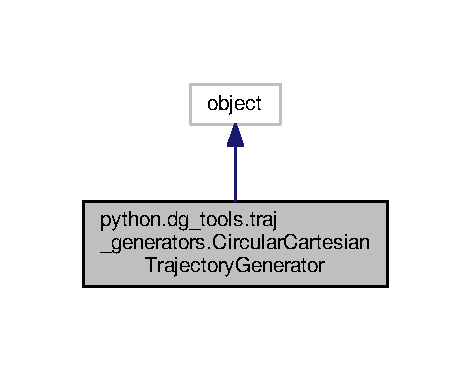
\includegraphics[width=226pt]{classpython_1_1dg__tools_1_1traj__generators_1_1CircularCartesianTrajectoryGenerator__inherit__graph}
\end{center}
\end{figure}


Collaboration diagram for python.\+dg\+\_\+tools.\+traj\+\_\+generators.\+Circular\+Cartesian\+Trajectory\+Generator\+:
\nopagebreak
\begin{figure}[H]
\begin{center}
\leavevmode
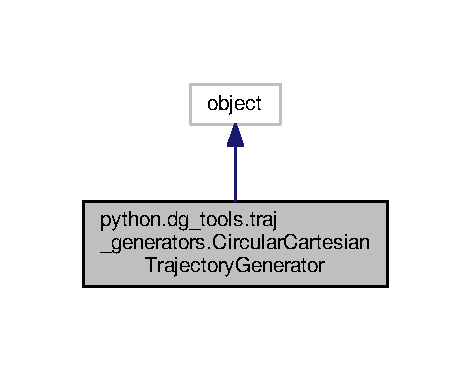
\includegraphics[width=226pt]{classpython_1_1dg__tools_1_1traj__generators_1_1CircularCartesianTrajectoryGenerator__coll__graph}
\end{center}
\end{figure}
\subsection*{Public Member Functions}
\begin{DoxyCompactItemize}
\item 
def {\bfseries \+\_\+\+\_\+init\+\_\+\+\_\+} (self, prefix=\char`\"{}\char`\"{}, time\+\_\+period=0.\+001)\hypertarget{classpython_1_1dg__tools_1_1traj__generators_1_1CircularCartesianTrajectoryGenerator_a306a71f14b3d5820ad0025e4309597fa}{}\label{classpython_1_1dg__tools_1_1traj__generators_1_1CircularCartesianTrajectoryGenerator_a306a71f14b3d5820ad0025e4309597fa}

\item 
def \hyperlink{classpython_1_1dg__tools_1_1traj__generators_1_1CircularCartesianTrajectoryGenerator_a5863b65052d601d51c1c4f7a7a51ef86}{set\+\_\+time\+\_\+period} (self, time\+\_\+period)\hypertarget{classpython_1_1dg__tools_1_1traj__generators_1_1CircularCartesianTrajectoryGenerator_a5863b65052d601d51c1c4f7a7a51ef86}{}\label{classpython_1_1dg__tools_1_1traj__generators_1_1CircularCartesianTrajectoryGenerator_a5863b65052d601d51c1c4f7a7a51ef86}

\begin{DoxyCompactList}\small\item\em set the time period to all oscillation entities \end{DoxyCompactList}\item 
def {\bfseries plug} (self, magnitude, omega, phase, bias)\hypertarget{classpython_1_1dg__tools_1_1traj__generators_1_1CircularCartesianTrajectoryGenerator_a7bad7e080c9ee06d59eef7225b8f2db0}{}\label{classpython_1_1dg__tools_1_1traj__generators_1_1CircularCartesianTrajectoryGenerator_a7bad7e080c9ee06d59eef7225b8f2db0}

\item 
def {\bfseries trace} (self, robot)\hypertarget{classpython_1_1dg__tools_1_1traj__generators_1_1CircularCartesianTrajectoryGenerator_a9374bc67e24fd8c8a1288fc30ec861d8}{}\label{classpython_1_1dg__tools_1_1traj__generators_1_1CircularCartesianTrajectoryGenerator_a9374bc67e24fd8c8a1288fc30ec861d8}

\end{DoxyCompactItemize}
\subsection*{Public Attributes}
\begin{DoxyCompactItemize}
\item 
{\bfseries time\+\_\+period}\hypertarget{classpython_1_1dg__tools_1_1traj__generators_1_1CircularCartesianTrajectoryGenerator_a01f19fbdfd5492d5d35d0debbf8ab89a}{}\label{classpython_1_1dg__tools_1_1traj__generators_1_1CircularCartesianTrajectoryGenerator_a01f19fbdfd5492d5d35d0debbf8ab89a}

\item 
{\bfseries prefix}\hypertarget{classpython_1_1dg__tools_1_1traj__generators_1_1CircularCartesianTrajectoryGenerator_ae65dea0551140899f125f67db065f911}{}\label{classpython_1_1dg__tools_1_1traj__generators_1_1CircularCartesianTrajectoryGenerator_ae65dea0551140899f125f67db065f911}

\item 
{\bfseries pi\+\_\+by\+\_\+2}\hypertarget{classpython_1_1dg__tools_1_1traj__generators_1_1CircularCartesianTrajectoryGenerator_a33454143d6c568fea94e58204c055857}{}\label{classpython_1_1dg__tools_1_1traj__generators_1_1CircularCartesianTrajectoryGenerator_a33454143d6c568fea94e58204c055857}

\item 
{\bfseries des\+\_\+pos\+\_\+xy}\hypertarget{classpython_1_1dg__tools_1_1traj__generators_1_1CircularCartesianTrajectoryGenerator_a7e1d9a9bebbf50965b0840ec4d41ecc2}{}\label{classpython_1_1dg__tools_1_1traj__generators_1_1CircularCartesianTrajectoryGenerator_a7e1d9a9bebbf50965b0840ec4d41ecc2}

\item 
{\bfseries des\+\_\+pos}\hypertarget{classpython_1_1dg__tools_1_1traj__generators_1_1CircularCartesianTrajectoryGenerator_a7bbe65759b9210c4762dc0dd73c9a4a5}{}\label{classpython_1_1dg__tools_1_1traj__generators_1_1CircularCartesianTrajectoryGenerator_a7bbe65759b9210c4762dc0dd73c9a4a5}

\item 
{\bfseries des\+\_\+vel\+\_\+xy}\hypertarget{classpython_1_1dg__tools_1_1traj__generators_1_1CircularCartesianTrajectoryGenerator_a3929cda646a0c9ddd9ef04c786564fe3}{}\label{classpython_1_1dg__tools_1_1traj__generators_1_1CircularCartesianTrajectoryGenerator_a3929cda646a0c9ddd9ef04c786564fe3}

\item 
{\bfseries des\+\_\+vel}\hypertarget{classpython_1_1dg__tools_1_1traj__generators_1_1CircularCartesianTrajectoryGenerator_a90de45b8eaab3b2672fe9783fe96cc86}{}\label{classpython_1_1dg__tools_1_1traj__generators_1_1CircularCartesianTrajectoryGenerator_a90de45b8eaab3b2672fe9783fe96cc86}

\end{DoxyCompactItemize}


\subsection{Detailed Description}
generates a circular circular\+\_\+trajectory\+\_\+generator 

The documentation for this class was generated from the following file\+:\begin{DoxyCompactItemize}
\item 
python/dg\+\_\+tools/\hyperlink{traj__generators_8py}{traj\+\_\+generators.\+py}\end{DoxyCompactItemize}

\hypertarget{classdynamicgraph_1_1sot_1_1ComImpedanceControl}{}\section{dynamicgraph\+:\+:sot\+:\+:Com\+Impedance\+Control Class Reference}
\label{classdynamicgraph_1_1sot_1_1ComImpedanceControl}\index{dynamicgraph\+::sot\+::\+Com\+Impedance\+Control@{dynamicgraph\+::sot\+::\+Com\+Impedance\+Control}}


Inheritance diagram for dynamicgraph\+:\+:sot\+:\+:Com\+Impedance\+Control\+:
\nopagebreak
\begin{figure}[H]
\begin{center}
\leavevmode
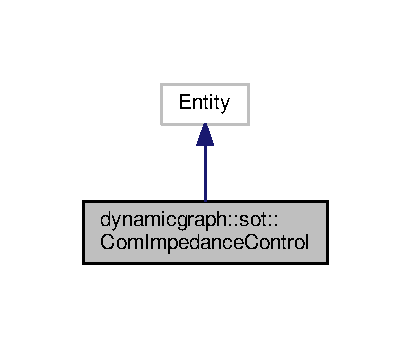
\includegraphics[width=197pt]{classdynamicgraph_1_1sot_1_1ComImpedanceControl__inherit__graph}
\end{center}
\end{figure}


Collaboration diagram for dynamicgraph\+:\+:sot\+:\+:Com\+Impedance\+Control\+:
\nopagebreak
\begin{figure}[H]
\begin{center}
\leavevmode
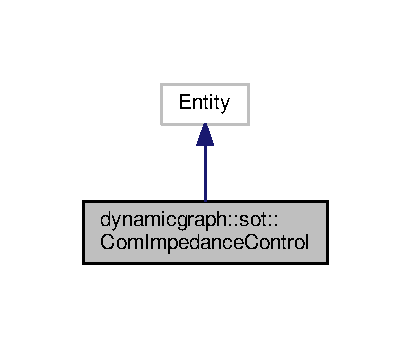
\includegraphics[width=197pt]{classdynamicgraph_1_1sot_1_1ComImpedanceControl__coll__graph}
\end{center}
\end{figure}
\subsection*{Public Member Functions}
\begin{DoxyCompactItemize}
\item 
{\bfseries Com\+Impedance\+Control} (const std\+::string \&name)\hypertarget{classdynamicgraph_1_1sot_1_1ComImpedanceControl_a1da4aa67c57a44b99f7923053af4bda4}{}\label{classdynamicgraph_1_1sot_1_1ComImpedanceControl_a1da4aa67c57a44b99f7923053af4bda4}

\item 
void {\bfseries init} (const double \&step)\hypertarget{classdynamicgraph_1_1sot_1_1ComImpedanceControl_a6d89dd52f34e28be576e98c920e0089a}{}\label{classdynamicgraph_1_1sot_1_1ComImpedanceControl_a6d89dd52f34e28be576e98c920e0089a}

\item 
virtual const std\+::string \& {\bfseries get\+Class\+Name} (void) const \hypertarget{classdynamicgraph_1_1sot_1_1ComImpedanceControl_a9cb84783c4bc60a5e45c1e57a538e8bb}{}\label{classdynamicgraph_1_1sot_1_1ComImpedanceControl_a9cb84783c4bc60a5e45c1e57a538e8bb}

\end{DoxyCompactItemize}
\subsection*{Public Attributes}
\begin{DoxyCompactItemize}
\item 
Signal\+Ptr$<$ dg\+::\+Vector, int $>$ {\bfseries Kp\+S\+IN}\hypertarget{classdynamicgraph_1_1sot_1_1ComImpedanceControl_a201e07d369283b70268a05cf60af1703}{}\label{classdynamicgraph_1_1sot_1_1ComImpedanceControl_a201e07d369283b70268a05cf60af1703}

\item 
Signal\+Ptr$<$ dg\+::\+Vector, int $>$ {\bfseries Kp\+Ang\+S\+IN}\hypertarget{classdynamicgraph_1_1sot_1_1ComImpedanceControl_a897667804ebe9d2d2159dcb357df73b5}{}\label{classdynamicgraph_1_1sot_1_1ComImpedanceControl_a897667804ebe9d2d2159dcb357df73b5}

\item 
Signal\+Ptr$<$ dg\+::\+Vector, int $>$ {\bfseries Kd\+Ang\+S\+IN}\hypertarget{classdynamicgraph_1_1sot_1_1ComImpedanceControl_ac12aca65f0111b3407635b1d40b29acc}{}\label{classdynamicgraph_1_1sot_1_1ComImpedanceControl_ac12aca65f0111b3407635b1d40b29acc}

\item 
Signal\+Ptr$<$ dg\+::\+Vector, int $>$ {\bfseries Kd\+S\+IN}\hypertarget{classdynamicgraph_1_1sot_1_1ComImpedanceControl_ae21ebdf77208ce22827b37c6a61ae021}{}\label{classdynamicgraph_1_1sot_1_1ComImpedanceControl_ae21ebdf77208ce22827b37c6a61ae021}

\item 
Signal\+Ptr$<$ dg\+::\+Vector, int $>$ {\bfseries position\+S\+IN}\hypertarget{classdynamicgraph_1_1sot_1_1ComImpedanceControl_a24095b41fc0963dcd32d8d334eabe887}{}\label{classdynamicgraph_1_1sot_1_1ComImpedanceControl_a24095b41fc0963dcd32d8d334eabe887}

\item 
Signal\+Ptr$<$ dg\+::\+Vector, int $>$ {\bfseries desiredposition\+S\+IN}\hypertarget{classdynamicgraph_1_1sot_1_1ComImpedanceControl_aedab4c4732d82e5aabcbbe7fc94ac221}{}\label{classdynamicgraph_1_1sot_1_1ComImpedanceControl_aedab4c4732d82e5aabcbbe7fc94ac221}

\item 
Signal\+Ptr$<$ dg\+::\+Vector, int $>$ {\bfseries biasedposition\+S\+IN}\hypertarget{classdynamicgraph_1_1sot_1_1ComImpedanceControl_ab3abe654a0fb2284f453a50cc0da4ede}{}\label{classdynamicgraph_1_1sot_1_1ComImpedanceControl_ab3abe654a0fb2284f453a50cc0da4ede}

\item 
Signal\+Ptr$<$ dg\+::\+Vector, int $>$ {\bfseries velocity\+S\+IN}\hypertarget{classdynamicgraph_1_1sot_1_1ComImpedanceControl_ab88a9c6ca1556c1db688b5fbeb84ce11}{}\label{classdynamicgraph_1_1sot_1_1ComImpedanceControl_ab88a9c6ca1556c1db688b5fbeb84ce11}

\item 
Signal\+Ptr$<$ dg\+::\+Vector, int $>$ {\bfseries desiredvelocity\+S\+IN}\hypertarget{classdynamicgraph_1_1sot_1_1ComImpedanceControl_a71711ceae0d997da7f3fc52e96337af2}{}\label{classdynamicgraph_1_1sot_1_1ComImpedanceControl_a71711ceae0d997da7f3fc52e96337af2}

\item 
Signal\+Ptr$<$ dg\+::\+Vector, int $>$ {\bfseries biasedvelocity\+S\+IN}\hypertarget{classdynamicgraph_1_1sot_1_1ComImpedanceControl_a5d785810c3b788f12ae73c006849b646}{}\label{classdynamicgraph_1_1sot_1_1ComImpedanceControl_a5d785810c3b788f12ae73c006849b646}

\item 
Signal\+Ptr$<$ dg\+::\+Vector, int $>$ {\bfseries inertia\+S\+IN}\hypertarget{classdynamicgraph_1_1sot_1_1ComImpedanceControl_a0479c944eaf6b939eb452f37db8f30e1}{}\label{classdynamicgraph_1_1sot_1_1ComImpedanceControl_a0479c944eaf6b939eb452f37db8f30e1}

\item 
Signal\+Ptr$<$ dg\+::\+Vector, int $>$ {\bfseries mass\+S\+IN}\hypertarget{classdynamicgraph_1_1sot_1_1ComImpedanceControl_aa0198dfe15bf749c468f78e87534b7f8}{}\label{classdynamicgraph_1_1sot_1_1ComImpedanceControl_aa0198dfe15bf749c468f78e87534b7f8}

\item 
Signal\+Ptr$<$ dg\+::\+Vector, int $>$ {\bfseries ori\+S\+IN}\hypertarget{classdynamicgraph_1_1sot_1_1ComImpedanceControl_a0d23f4e82a310785c1c71e8ac7d36ba6}{}\label{classdynamicgraph_1_1sot_1_1ComImpedanceControl_a0d23f4e82a310785c1c71e8ac7d36ba6}

\item 
Signal\+Ptr$<$ dg\+::\+Vector, int $>$ {\bfseries desori\+S\+IN}\hypertarget{classdynamicgraph_1_1sot_1_1ComImpedanceControl_af79eff4807396ddc44fc8883132a1104}{}\label{classdynamicgraph_1_1sot_1_1ComImpedanceControl_af79eff4807396ddc44fc8883132a1104}

\item 
Signal\+Ptr$<$ dg\+::\+Vector, int $>$ {\bfseries angvel\+S\+IN}\hypertarget{classdynamicgraph_1_1sot_1_1ComImpedanceControl_a3dd8d09cda15382ebcbd81e3fadb9c9d}{}\label{classdynamicgraph_1_1sot_1_1ComImpedanceControl_a3dd8d09cda15382ebcbd81e3fadb9c9d}

\item 
Signal\+Ptr$<$ dg\+::\+Vector, int $>$ {\bfseries desiredangvel\+S\+IN}\hypertarget{classdynamicgraph_1_1sot_1_1ComImpedanceControl_a892a7fd19768ef54c3296d9e79b29b59}{}\label{classdynamicgraph_1_1sot_1_1ComImpedanceControl_a892a7fd19768ef54c3296d9e79b29b59}

\item 
Signal\+Ptr$<$ dg\+::\+Vector, int $>$ {\bfseries feedforwardforce\+S\+IN}\hypertarget{classdynamicgraph_1_1sot_1_1ComImpedanceControl_ae90c60c739651d9bacec332041cb21ef}{}\label{classdynamicgraph_1_1sot_1_1ComImpedanceControl_ae90c60c739651d9bacec332041cb21ef}

\item 
Signal\+Ptr$<$ dg\+::\+Vector, int $>$ {\bfseries feedforwardtorques\+S\+IN}\hypertarget{classdynamicgraph_1_1sot_1_1ComImpedanceControl_a4c30e7bfd1c1f85969d8b5624c0322d4}{}\label{classdynamicgraph_1_1sot_1_1ComImpedanceControl_a4c30e7bfd1c1f85969d8b5624c0322d4}

\item 
Signal\+Ptr$<$ dg\+::\+Vector, int $>$ {\bfseries cntsensor\+S\+IN}\hypertarget{classdynamicgraph_1_1sot_1_1ComImpedanceControl_a2108744924ac42d751c5ff9b7e87007a}{}\label{classdynamicgraph_1_1sot_1_1ComImpedanceControl_a2108744924ac42d751c5ff9b7e87007a}

\item 
Signal\+Ptr$<$ dg\+::\+Vector, int $>$ {\bfseries thrcntvalue\+S\+IN}\hypertarget{classdynamicgraph_1_1sot_1_1ComImpedanceControl_a8549527d47b1a62e59c87d91b00fc070}{}\label{classdynamicgraph_1_1sot_1_1ComImpedanceControl_a8549527d47b1a62e59c87d91b00fc070}

\item 
Signal\+Ptr$<$ dg\+::\+Vector, int $>$ {\bfseries lqrerror\+S\+IN}\hypertarget{classdynamicgraph_1_1sot_1_1ComImpedanceControl_aaa8e1de6e7501d1cbf4ce25cdd4cb2a5}{}\label{classdynamicgraph_1_1sot_1_1ComImpedanceControl_aaa8e1de6e7501d1cbf4ce25cdd4cb2a5}

\item 
Signal\+Ptr$<$ dg\+::\+Vector, int $>$ {\bfseries lqrgain\+S\+IN}\hypertarget{classdynamicgraph_1_1sot_1_1ComImpedanceControl_aef7e31d4f6ca57c037ff3f848f608252}{}\label{classdynamicgraph_1_1sot_1_1ComImpedanceControl_aef7e31d4f6ca57c037ff3f848f608252}

\item 
Signal\+Ptr$<$ dg\+::\+Vector, int $>$ {\bfseries lctrl\+S\+IN}\hypertarget{classdynamicgraph_1_1sot_1_1ComImpedanceControl_a2b9f069f4a8bb20e0daa850cd0c556b2}{}\label{classdynamicgraph_1_1sot_1_1ComImpedanceControl_a2b9f069f4a8bb20e0daa850cd0c556b2}

\item 
Signal\+Ptr$<$ dg\+::\+Vector, int $>$ {\bfseries actrl\+S\+IN}\hypertarget{classdynamicgraph_1_1sot_1_1ComImpedanceControl_abefb5e83b41571348605b35c2f22fab8}{}\label{classdynamicgraph_1_1sot_1_1ComImpedanceControl_abefb5e83b41571348605b35c2f22fab8}

\item 
Signal\+Ptr$<$ dg\+::\+Matrix, int $>$ {\bfseries hess\+S\+IN}\hypertarget{classdynamicgraph_1_1sot_1_1ComImpedanceControl_af9dc094dc62588a6573dc0aab10eb750}{}\label{classdynamicgraph_1_1sot_1_1ComImpedanceControl_af9dc094dc62588a6573dc0aab10eb750}

\item 
Signal\+Ptr$<$ dg\+::\+Vector, int $>$ {\bfseries g0\+S\+IN}\hypertarget{classdynamicgraph_1_1sot_1_1ComImpedanceControl_a5ae4138c8e194539c08b1657c580dd1d}{}\label{classdynamicgraph_1_1sot_1_1ComImpedanceControl_a5ae4138c8e194539c08b1657c580dd1d}

\item 
Signal\+Ptr$<$ dg\+::\+Matrix, int $>$ {\bfseries ce\+S\+IN}\hypertarget{classdynamicgraph_1_1sot_1_1ComImpedanceControl_a4e41f5bc2743bba9d2022af27cf9cc0b}{}\label{classdynamicgraph_1_1sot_1_1ComImpedanceControl_a4e41f5bc2743bba9d2022af27cf9cc0b}

\item 
Signal\+Ptr$<$ dg\+::\+Matrix, int $>$ {\bfseries ci\+S\+IN}\hypertarget{classdynamicgraph_1_1sot_1_1ComImpedanceControl_a481e26828cbee36931211b744738040c}{}\label{classdynamicgraph_1_1sot_1_1ComImpedanceControl_a481e26828cbee36931211b744738040c}

\item 
Signal\+Ptr$<$ dg\+::\+Vector, int $>$ {\bfseries ci0\+S\+IN}\hypertarget{classdynamicgraph_1_1sot_1_1ComImpedanceControl_a1d52509ce8e4eacf7d8808b64f7a3520}{}\label{classdynamicgraph_1_1sot_1_1ComImpedanceControl_a1d52509ce8e4eacf7d8808b64f7a3520}

\item 
Signal\+Ptr$<$ dg\+::\+Matrix, int $>$ {\bfseries reg\+S\+IN}\hypertarget{classdynamicgraph_1_1sot_1_1ComImpedanceControl_a7d782d12844d013cc502defbf5eb0a3c}{}\label{classdynamicgraph_1_1sot_1_1ComImpedanceControl_a7d782d12844d013cc502defbf5eb0a3c}

\item 
Signal\+Ptr$<$ dg\+::\+Vector, int $>$ {\bfseries absendeffpos\+S\+IN}\hypertarget{classdynamicgraph_1_1sot_1_1ComImpedanceControl_a1dfac0859d4c86d6ba0e8f960c979d78}{}\label{classdynamicgraph_1_1sot_1_1ComImpedanceControl_a1dfac0859d4c86d6ba0e8f960c979d78}

\item 
Signal\+Ptr$<$ dg\+::\+Vector, int $>$ {\bfseries absendeffvel\+S\+IN}\hypertarget{classdynamicgraph_1_1sot_1_1ComImpedanceControl_a6f164fcd07ce3c69a5f5021cf9069202}{}\label{classdynamicgraph_1_1sot_1_1ComImpedanceControl_a6f164fcd07ce3c69a5f5021cf9069202}

\item 
Signal\+Ptr$<$ dg\+::\+Vector, int $>$ \hyperlink{classdynamicgraph_1_1sot_1_1ComImpedanceControl_ae4f3968a33b09493a9e436d02b65290f}{leglengthfl\+S\+IN}\hypertarget{classdynamicgraph_1_1sot_1_1ComImpedanceControl_ae4f3968a33b09493a9e436d02b65290f}{}\label{classdynamicgraph_1_1sot_1_1ComImpedanceControl_ae4f3968a33b09493a9e436d02b65290f}

\begin{DoxyCompactList}\small\item\em for balancing taks on a planck \end{DoxyCompactList}\item 
Signal\+Ptr$<$ dg\+::\+Vector, int $>$ {\bfseries leglengthhl\+S\+IN}\hypertarget{classdynamicgraph_1_1sot_1_1ComImpedanceControl_a5c2b28a82349231a8a1b7a583b679edf}{}\label{classdynamicgraph_1_1sot_1_1ComImpedanceControl_a5c2b28a82349231a8a1b7a583b679edf}

\item 
Signal\+Time\+Dependent$<$ dg\+::\+Vector, int $>$ {\bfseries control\+S\+O\+UT}\hypertarget{classdynamicgraph_1_1sot_1_1ComImpedanceControl_a32a8354c781bb3f98c1b6cddecf8c9c1}{}\label{classdynamicgraph_1_1sot_1_1ComImpedanceControl_a32a8354c781bb3f98c1b6cddecf8c9c1}

\item 
Signal\+Time\+Dependent$<$ dg\+::\+Vector, int $>$ {\bfseries angcontrol\+S\+O\+UT}\hypertarget{classdynamicgraph_1_1sot_1_1ComImpedanceControl_a2702e983aa2f5d0f5ead23475acef432}{}\label{classdynamicgraph_1_1sot_1_1ComImpedanceControl_a2702e983aa2f5d0f5ead23475acef432}

\item 
Signal\+Time\+Dependent$<$ dg\+::\+Vector, int $>$ {\bfseries Set\+Pos\+Bias\+S\+O\+UT}\hypertarget{classdynamicgraph_1_1sot_1_1ComImpedanceControl_a1db5962c288566a15fbcf6f1c42ca63b}{}\label{classdynamicgraph_1_1sot_1_1ComImpedanceControl_a1db5962c288566a15fbcf6f1c42ca63b}

\item 
Signal\+Time\+Dependent$<$ dg\+::\+Vector, int $>$ {\bfseries Set\+Vel\+Bias\+S\+O\+UT}\hypertarget{classdynamicgraph_1_1sot_1_1ComImpedanceControl_a963b7859b6827e81ab3e6bf921d391d7}{}\label{classdynamicgraph_1_1sot_1_1ComImpedanceControl_a963b7859b6827e81ab3e6bf921d391d7}

\item 
Signal\+Time\+Dependent$<$ dg\+::\+Vector, int $>$ {\bfseries Thr\+Cnt\+Sensor\+S\+O\+UT}\hypertarget{classdynamicgraph_1_1sot_1_1ComImpedanceControl_a53d98df81cb5a2dcd2b493e8dcdd7fb7}{}\label{classdynamicgraph_1_1sot_1_1ComImpedanceControl_a53d98df81cb5a2dcd2b493e8dcdd7fb7}

\item 
Signal\+Time\+Dependent$<$ dg\+::\+Vector, int $>$ {\bfseries lqrcontrol\+S\+O\+UT}\hypertarget{classdynamicgraph_1_1sot_1_1ComImpedanceControl_ae7a1ce6a36b7af188b8b6d82d5443da2}{}\label{classdynamicgraph_1_1sot_1_1ComImpedanceControl_ae7a1ce6a36b7af188b8b6d82d5443da2}

\item 
Signal\+Time\+Dependent$<$ dg\+::\+Vector, int $>$ {\bfseries endefflqrcontrol\+S\+O\+UT}\hypertarget{classdynamicgraph_1_1sot_1_1ComImpedanceControl_ac8d0213a39a324f9292bff2c62965db0}{}\label{classdynamicgraph_1_1sot_1_1ComImpedanceControl_ac8d0213a39a324f9292bff2c62965db0}

\item 
Signal\+Time\+Dependent$<$ dg\+::\+Vector, int $>$ {\bfseries wbcontrol\+S\+O\+UT}\hypertarget{classdynamicgraph_1_1sot_1_1ComImpedanceControl_a75db64990cf315dd752c7569a93bac18}{}\label{classdynamicgraph_1_1sot_1_1ComImpedanceControl_a75db64990cf315dd752c7569a93bac18}

\item 
Signal\+Time\+Dependent$<$ dg\+::\+Vector, int $>$ {\bfseries descompos\+S\+O\+UT}\hypertarget{classdynamicgraph_1_1sot_1_1ComImpedanceControl_a9c1a87a218a2979a252da7ed8c12c2f1}{}\label{classdynamicgraph_1_1sot_1_1ComImpedanceControl_a9c1a87a218a2979a252da7ed8c12c2f1}

\end{DoxyCompactItemize}
\subsection*{Static Public Attributes}
\begin{DoxyCompactItemize}
\item 
static const double {\bfseries T\+I\+M\+E\+\_\+\+S\+T\+E\+P\+\_\+\+D\+E\+F\+A\+U\+LT}\hypertarget{classdynamicgraph_1_1sot_1_1ComImpedanceControl_ad065fb4f254e2c48ba3d70fb3cb2b3cb}{}\label{classdynamicgraph_1_1sot_1_1ComImpedanceControl_ad065fb4f254e2c48ba3d70fb3cb2b3cb}

\item 
static const std\+::string {\bfseries C\+L\+A\+S\+S\+\_\+\+N\+A\+ME}\hypertarget{classdynamicgraph_1_1sot_1_1ComImpedanceControl_a62e724ec127c6d67806f0e0b601a3e9f}{}\label{classdynamicgraph_1_1sot_1_1ComImpedanceControl_a62e724ec127c6d67806f0e0b601a3e9f}

\end{DoxyCompactItemize}
\subsection*{Protected Member Functions}
\begin{DoxyCompactItemize}
\item 
double \& {\bfseries setsize} (int dimension)\hypertarget{classdynamicgraph_1_1sot_1_1ComImpedanceControl_a347f5be0bd9167793b5ca5cfe1fcee1b}{}\label{classdynamicgraph_1_1sot_1_1ComImpedanceControl_a347f5be0bd9167793b5ca5cfe1fcee1b}

\item 
dg\+::\+Vector \& {\bfseries return\+\_\+control\+\_\+torques} (dg\+::\+Vector \&tau, int t)\hypertarget{classdynamicgraph_1_1sot_1_1ComImpedanceControl_a7b2c7270cb18bd1856f11c86b7937ab3}{}\label{classdynamicgraph_1_1sot_1_1ComImpedanceControl_a7b2c7270cb18bd1856f11c86b7937ab3}

\item 
dg\+::\+Vector \& {\bfseries return\+\_\+angcontrol\+\_\+torques} (dg\+::\+Vector \&angtau, int t)\hypertarget{classdynamicgraph_1_1sot_1_1ComImpedanceControl_a3069704cb14b9729d52b97f4466f82e8}{}\label{classdynamicgraph_1_1sot_1_1ComImpedanceControl_a3069704cb14b9729d52b97f4466f82e8}

\item 
dg\+::\+Vector \& {\bfseries set\+\_\+pos\+\_\+bias} (dg\+::\+Vector \&pos\+\_\+bias, int t)\hypertarget{classdynamicgraph_1_1sot_1_1ComImpedanceControl_aead1e61d4ffea75a0f0036b086f8fd8a}{}\label{classdynamicgraph_1_1sot_1_1ComImpedanceControl_aead1e61d4ffea75a0f0036b086f8fd8a}

\item 
dg\+::\+Vector \& {\bfseries set\+\_\+vel\+\_\+bias} (dg\+::\+Vector \&vel\+\_\+bias, int t)\hypertarget{classdynamicgraph_1_1sot_1_1ComImpedanceControl_a0b09ed32454cbecee116b2ac229a7b44}{}\label{classdynamicgraph_1_1sot_1_1ComImpedanceControl_a0b09ed32454cbecee116b2ac229a7b44}

\item 
dg\+::\+Vector \& {\bfseries threshold\+\_\+cnt\+\_\+sensor} (dg\+::\+Vector \&thr\+\_\+cnt\+\_\+sensor, int t)\hypertarget{classdynamicgraph_1_1sot_1_1ComImpedanceControl_a5bf7ea6d98e8aba42ec6fa782fbe0b4c}{}\label{classdynamicgraph_1_1sot_1_1ComImpedanceControl_a5bf7ea6d98e8aba42ec6fa782fbe0b4c}

\item 
dg\+::\+Vector \& \hyperlink{classdynamicgraph_1_1sot_1_1ComImpedanceControl_a6c33c88c2a5ae61dbde00dbd001355ca}{return\+\_\+lqr\+\_\+tau} (dg\+::\+Vector \&lqrtau, int t)
\item 
dg\+::\+Vector \& \hyperlink{classdynamicgraph_1_1sot_1_1ComImpedanceControl_a3df6780c7565af64536541c04c7e55f4}{return\+\_\+end\+\_\+eff\+\_\+lqr\+\_\+tau} (dg\+::\+Vector \&end\+\_\+eff\+\_\+lqr\+\_\+tau, int t)
\item 
dg\+::\+Vector \& {\bfseries compute\+\_\+end\+\_\+eff\+\_\+forces} (dg\+::\+Vector \&end\+\_\+forces, int t)\hypertarget{classdynamicgraph_1_1sot_1_1ComImpedanceControl_ad490f975131e2a420778e843e7b76c81}{}\label{classdynamicgraph_1_1sot_1_1ComImpedanceControl_ad490f975131e2a420778e843e7b76c81}

\item 
dg\+::\+Vector \& {\bfseries compute\+\_\+des\+\_\+com\+\_\+pos} (dg\+::\+Vector \&des\+\_\+com\+\_\+pos, int t)\hypertarget{classdynamicgraph_1_1sot_1_1ComImpedanceControl_ab16f1f8744e0a844215b5c9a6e46ac32}{}\label{classdynamicgraph_1_1sot_1_1ComImpedanceControl_ab16f1f8744e0a844215b5c9a6e46ac32}

\end{DoxyCompactItemize}
\subsection*{Protected Attributes}
\begin{DoxyCompactItemize}
\item 
double {\bfseries Time\+Step}\hypertarget{classdynamicgraph_1_1sot_1_1ComImpedanceControl_a8da858067d374ebf6ae8273bfd2f68a9}{}\label{classdynamicgraph_1_1sot_1_1ComImpedanceControl_a8da858067d374ebf6ae8273bfd2f68a9}

\item 
dg\+::\+Vector {\bfseries pos\+\_\+error}\hypertarget{classdynamicgraph_1_1sot_1_1ComImpedanceControl_a2949f183f4d327cd276c970c6518a5d1}{}\label{classdynamicgraph_1_1sot_1_1ComImpedanceControl_a2949f183f4d327cd276c970c6518a5d1}

\item 
dg\+::\+Vector {\bfseries vel\+\_\+error}\hypertarget{classdynamicgraph_1_1sot_1_1ComImpedanceControl_a969ff175749f7fa941b113521ce21f16}{}\label{classdynamicgraph_1_1sot_1_1ComImpedanceControl_a969ff175749f7fa941b113521ce21f16}

\item 
dg\+::\+Vector {\bfseries h\+\_\+error}\hypertarget{classdynamicgraph_1_1sot_1_1ComImpedanceControl_a98f04f17826d362336933d88ee1e0a72}{}\label{classdynamicgraph_1_1sot_1_1ComImpedanceControl_a98f04f17826d362336933d88ee1e0a72}

\item 
dg\+::\+Vector {\bfseries ori\+\_\+error}\hypertarget{classdynamicgraph_1_1sot_1_1ComImpedanceControl_abe47c8c83c1d6da3ce4e41200f6a41d1}{}\label{classdynamicgraph_1_1sot_1_1ComImpedanceControl_abe47c8c83c1d6da3ce4e41200f6a41d1}

\item 
dg\+::\+Vector {\bfseries position\+\_\+bias}\hypertarget{classdynamicgraph_1_1sot_1_1ComImpedanceControl_ad860ad830c8182511376bce58a2d6f93}{}\label{classdynamicgraph_1_1sot_1_1ComImpedanceControl_ad860ad830c8182511376bce58a2d6f93}

\item 
dg\+::\+Vector {\bfseries velocity\+\_\+bias}\hypertarget{classdynamicgraph_1_1sot_1_1ComImpedanceControl_a1be85794682702c8190b9ae8e9db7e69}{}\label{classdynamicgraph_1_1sot_1_1ComImpedanceControl_a1be85794682702c8190b9ae8e9db7e69}

\item 
float {\bfseries w1}\hypertarget{classdynamicgraph_1_1sot_1_1ComImpedanceControl_a56da2479df7879279c2af40302fdeac6}{}\label{classdynamicgraph_1_1sot_1_1ComImpedanceControl_a56da2479df7879279c2af40302fdeac6}

\item 
float {\bfseries w2}\hypertarget{classdynamicgraph_1_1sot_1_1ComImpedanceControl_a58b0640068d902bea7dac9044e1f7c34}{}\label{classdynamicgraph_1_1sot_1_1ComImpedanceControl_a58b0640068d902bea7dac9044e1f7c34}

\item 
dg\+::\+Vector {\bfseries ce0}\hypertarget{classdynamicgraph_1_1sot_1_1ComImpedanceControl_a2ef7f8b25bf9ff36f632d12567ca327f}{}\label{classdynamicgraph_1_1sot_1_1ComImpedanceControl_a2ef7f8b25bf9ff36f632d12567ca327f}

\item 
dg\+::\+Vector {\bfseries end\+\_\+forces}\hypertarget{classdynamicgraph_1_1sot_1_1ComImpedanceControl_aa9a8673fd9925a90575cb86843a0bd22}{}\label{classdynamicgraph_1_1sot_1_1ComImpedanceControl_aa9a8673fd9925a90575cb86843a0bd22}

\item 
dg\+::\+Matrix {\bfseries hess\+\_\+new}\hypertarget{classdynamicgraph_1_1sot_1_1ComImpedanceControl_a94b718d59be0c1b7e91a1024e92adb1f}{}\label{classdynamicgraph_1_1sot_1_1ComImpedanceControl_a94b718d59be0c1b7e91a1024e92adb1f}

\item 
dg\+::\+Vector {\bfseries g0\+\_\+new}\hypertarget{classdynamicgraph_1_1sot_1_1ComImpedanceControl_a122b245fd649650d41573fb8f3298c7c}{}\label{classdynamicgraph_1_1sot_1_1ComImpedanceControl_a122b245fd649650d41573fb8f3298c7c}

\item 
dg\+::\+Matrix {\bfseries ce\+\_\+new}\hypertarget{classdynamicgraph_1_1sot_1_1ComImpedanceControl_a02172ace50e863a00368cba1b54b7d86}{}\label{classdynamicgraph_1_1sot_1_1ComImpedanceControl_a02172ace50e863a00368cba1b54b7d86}

\item 
dg\+::\+Matrix {\bfseries ci\+\_\+new}\hypertarget{classdynamicgraph_1_1sot_1_1ComImpedanceControl_a5e068407f7dbcb0a0604b2d63b49a095}{}\label{classdynamicgraph_1_1sot_1_1ComImpedanceControl_a5e068407f7dbcb0a0604b2d63b49a095}

\item 
Eigen\+::\+Quad\+Prog\+Dense {\bfseries qp}\hypertarget{classdynamicgraph_1_1sot_1_1ComImpedanceControl_a62a7c1d638782e8a5b14d322b5ab7b68}{}\label{classdynamicgraph_1_1sot_1_1ComImpedanceControl_a62a7c1d638782e8a5b14d322b5ab7b68}

\item 
Eigen\+::\+Quaternion$<$ double $>$ {\bfseries ori\+\_\+quat}\hypertarget{classdynamicgraph_1_1sot_1_1ComImpedanceControl_ad6c9efd3df56a908868272b5303f7266}{}\label{classdynamicgraph_1_1sot_1_1ComImpedanceControl_ad6c9efd3df56a908868272b5303f7266}

\item 
Eigen\+::\+Quaternion$<$ double $>$ {\bfseries des\+\_\+ori\+\_\+quat}\hypertarget{classdynamicgraph_1_1sot_1_1ComImpedanceControl_ab80ec2f42c578add2f40d77626be65fe}{}\label{classdynamicgraph_1_1sot_1_1ComImpedanceControl_ab80ec2f42c578add2f40d77626be65fe}

\item 
Eigen\+::\+Quaternion$<$ double $>$ {\bfseries ori\+\_\+error\+\_\+quat}\hypertarget{classdynamicgraph_1_1sot_1_1ComImpedanceControl_ac82f3d6ac9b351cc5a55ecf87c4cfae9}{}\label{classdynamicgraph_1_1sot_1_1ComImpedanceControl_ac82f3d6ac9b351cc5a55ecf87c4cfae9}

\item 
Eigen\+::\+Matrix$<$ double, 3, 3 $>$ {\bfseries ori\+\_\+se3}\hypertarget{classdynamicgraph_1_1sot_1_1ComImpedanceControl_ac17086e0eb3e694777e260e3a75eddab}{}\label{classdynamicgraph_1_1sot_1_1ComImpedanceControl_ac17086e0eb3e694777e260e3a75eddab}

\item 
Eigen\+::\+Matrix$<$ double, 3, 3 $>$ {\bfseries des\+\_\+ori\+\_\+se3}\hypertarget{classdynamicgraph_1_1sot_1_1ComImpedanceControl_ad10ecee50cccec45df7cc7fb2237d401}{}\label{classdynamicgraph_1_1sot_1_1ComImpedanceControl_ad10ecee50cccec45df7cc7fb2237d401}

\item 
Eigen\+::\+Matrix$<$ double, 3, 3 $>$ {\bfseries ori\+\_\+error\+\_\+se3}\hypertarget{classdynamicgraph_1_1sot_1_1ComImpedanceControl_a41e3f9435b73e68dd74560f1c3bf63a0}{}\label{classdynamicgraph_1_1sot_1_1ComImpedanceControl_a41e3f9435b73e68dd74560f1c3bf63a0}

\item 
dg\+::\+Vector {\bfseries diff}\hypertarget{classdynamicgraph_1_1sot_1_1ComImpedanceControl_aeda26b55aea8fe76f80e7695261b3a70}{}\label{classdynamicgraph_1_1sot_1_1ComImpedanceControl_aeda26b55aea8fe76f80e7695261b3a70}

\item 
Eigen\+::\+Matrix\+Xd {\bfseries K}\hypertarget{classdynamicgraph_1_1sot_1_1ComImpedanceControl_a7aac863f6fa45fa5184edcf6ab72d9b4}{}\label{classdynamicgraph_1_1sot_1_1ComImpedanceControl_a7aac863f6fa45fa5184edcf6ab72d9b4}

\item 
Eigen\+::\+Vector\+Xd {\bfseries delta\+\_\+x}\hypertarget{classdynamicgraph_1_1sot_1_1ComImpedanceControl_a7188ac36d781601dbe470aba833aaf6d}{}\label{classdynamicgraph_1_1sot_1_1ComImpedanceControl_a7188ac36d781601dbe470aba833aaf6d}

\item 
Eigen\+::\+Vector3d {\bfseries lqr\+\_\+pos\+\_\+error}\hypertarget{classdynamicgraph_1_1sot_1_1ComImpedanceControl_aeae7cde8a947ee772c31411a9a657ddb}{}\label{classdynamicgraph_1_1sot_1_1ComImpedanceControl_aeae7cde8a947ee772c31411a9a657ddb}

\item 
Eigen\+::\+Vector3d {\bfseries lqr\+\_\+vel\+\_\+error}\hypertarget{classdynamicgraph_1_1sot_1_1ComImpedanceControl_aa70d1dc78aed0428cb91df54bbbaf4e7}{}\label{classdynamicgraph_1_1sot_1_1ComImpedanceControl_aa70d1dc78aed0428cb91df54bbbaf4e7}

\item 
Eigen\+::\+Vector4d {\bfseries lqr\+\_\+ori\+\_\+error}\hypertarget{classdynamicgraph_1_1sot_1_1ComImpedanceControl_a4c8bd9593acac96b450835102d825a03}{}\label{classdynamicgraph_1_1sot_1_1ComImpedanceControl_a4c8bd9593acac96b450835102d825a03}

\item 
Eigen\+::\+Vector3d {\bfseries lqr\+\_\+ang\+\_\+vel\+\_\+error}\hypertarget{classdynamicgraph_1_1sot_1_1ComImpedanceControl_a879dc29e6909c5d54ce92dd654977c54}{}\label{classdynamicgraph_1_1sot_1_1ComImpedanceControl_a879dc29e6909c5d54ce92dd654977c54}

\item 
Eigen\+::\+Vector\+Xd {\bfseries f\+\_\+des}\hypertarget{classdynamicgraph_1_1sot_1_1ComImpedanceControl_ae95d848a425c378ae8025898b2505c86}{}\label{classdynamicgraph_1_1sot_1_1ComImpedanceControl_ae95d848a425c378ae8025898b2505c86}

\item 
int {\bfseries init\+\_\+flag\+\_\+pos}\hypertarget{classdynamicgraph_1_1sot_1_1ComImpedanceControl_aad0b9dd5b46a9e326c53b96623f506da}{}\label{classdynamicgraph_1_1sot_1_1ComImpedanceControl_aad0b9dd5b46a9e326c53b96623f506da}

\item 
int {\bfseries init\+\_\+flag\+\_\+vel}\hypertarget{classdynamicgraph_1_1sot_1_1ComImpedanceControl_adbcd9f6d659cec3ad88ad33650b11a1c}{}\label{classdynamicgraph_1_1sot_1_1ComImpedanceControl_adbcd9f6d659cec3ad88ad33650b11a1c}

\item 
int {\bfseries isbiasset}\hypertarget{classdynamicgraph_1_1sot_1_1ComImpedanceControl_a6efb1e7498082fd3461fe92efe5a4bb3}{}\label{classdynamicgraph_1_1sot_1_1ComImpedanceControl_a6efb1e7498082fd3461fe92efe5a4bb3}

\item 
int {\bfseries safetyswitch}\hypertarget{classdynamicgraph_1_1sot_1_1ComImpedanceControl_a84ad2783ad21be7b34dd1a322bef731c}{}\label{classdynamicgraph_1_1sot_1_1ComImpedanceControl_a84ad2783ad21be7b34dd1a322bef731c}

\item 
int {\bfseries t\+\_\+start}\hypertarget{classdynamicgraph_1_1sot_1_1ComImpedanceControl_a4bd858093bc5d0af1d1eaa44b9c7c23a}{}\label{classdynamicgraph_1_1sot_1_1ComImpedanceControl_a4bd858093bc5d0af1d1eaa44b9c7c23a}

\item 
int {\bfseries bias\+\_\+time}\hypertarget{classdynamicgraph_1_1sot_1_1ComImpedanceControl_ab58f493dbeb2cfdce14681cd604a0788}{}\label{classdynamicgraph_1_1sot_1_1ComImpedanceControl_ab58f493dbeb2cfdce14681cd604a0788}

\end{DoxyCompactItemize}


\subsection{Member Function Documentation}
\index{dynamicgraph\+::sot\+::\+Com\+Impedance\+Control@{dynamicgraph\+::sot\+::\+Com\+Impedance\+Control}!return\+\_\+end\+\_\+eff\+\_\+lqr\+\_\+tau@{return\+\_\+end\+\_\+eff\+\_\+lqr\+\_\+tau}}
\index{return\+\_\+end\+\_\+eff\+\_\+lqr\+\_\+tau@{return\+\_\+end\+\_\+eff\+\_\+lqr\+\_\+tau}!dynamicgraph\+::sot\+::\+Com\+Impedance\+Control@{dynamicgraph\+::sot\+::\+Com\+Impedance\+Control}}
\subsubsection[{\texorpdfstring{return\+\_\+end\+\_\+eff\+\_\+lqr\+\_\+tau(dg\+::\+Vector \&end\+\_\+eff\+\_\+lqr\+\_\+tau, int t)}{return_end_eff_lqr_tau(dg::Vector &end_eff_lqr_tau, int t)}}]{\setlength{\rightskip}{0pt plus 5cm}dynamicgraph\+::\+Vector \& Com\+Impedance\+Control\+::return\+\_\+end\+\_\+eff\+\_\+lqr\+\_\+tau (
\begin{DoxyParamCaption}
\item[{dg\+::\+Vector \&}]{end\+\_\+eff\+\_\+lqr\+\_\+tau, }
\item[{int}]{t}
\end{DoxyParamCaption}
)\hspace{0.3cm}{\ttfamily [protected]}}\hypertarget{classdynamicgraph_1_1sot_1_1ComImpedanceControl_a3df6780c7565af64536541c04c7e55f4}{}\label{classdynamicgraph_1_1sot_1_1ComImpedanceControl_a3df6780c7565af64536541c04c7e55f4}
this method computes the desired forces at the end effector based on the plan using lqr gains computated with orientation control \index{dynamicgraph\+::sot\+::\+Com\+Impedance\+Control@{dynamicgraph\+::sot\+::\+Com\+Impedance\+Control}!return\+\_\+lqr\+\_\+tau@{return\+\_\+lqr\+\_\+tau}}
\index{return\+\_\+lqr\+\_\+tau@{return\+\_\+lqr\+\_\+tau}!dynamicgraph\+::sot\+::\+Com\+Impedance\+Control@{dynamicgraph\+::sot\+::\+Com\+Impedance\+Control}}
\subsubsection[{\texorpdfstring{return\+\_\+lqr\+\_\+tau(dg\+::\+Vector \&lqrtau, int t)}{return_lqr_tau(dg::Vector &lqrtau, int t)}}]{\setlength{\rightskip}{0pt plus 5cm}dynamicgraph\+::\+Vector \& Com\+Impedance\+Control\+::return\+\_\+lqr\+\_\+tau (
\begin{DoxyParamCaption}
\item[{dg\+::\+Vector \&}]{lqrtau, }
\item[{int}]{t}
\end{DoxyParamCaption}
)\hspace{0.3cm}{\ttfamily [protected]}}\hypertarget{classdynamicgraph_1_1sot_1_1ComImpedanceControl_a6c33c88c2a5ae61dbde00dbd001355ca}{}\label{classdynamicgraph_1_1sot_1_1ComImpedanceControl_a6c33c88c2a5ae61dbde00dbd001355ca}
This method carries out a matrix multiplication of lqr gains obtained from the dynamic planner. lqr\+\_\+matrix $\ast$ \mbox{[}\mbox{[}com\+\_\+error\mbox{]}, \mbox{[}lmom\+\_\+error\mbox{]}, \mbox{[}ori\+\_\+error\mbox{]}, \mbox{[}amom\+\_\+error\mbox{]}\mbox{]} 

The documentation for this class was generated from the following files\+:\begin{DoxyCompactItemize}
\item 
include/dg\+\_\+tools/\+Com\+Impedance\+Control/\hyperlink{ComImpedanceController_8hpp}{Com\+Impedance\+Controller.\+hpp}\item 
src/com\+\_\+impedance\+\_\+control/com\+\_\+impedance\+\_\+controller.\+cpp\end{DoxyCompactItemize}

\hypertarget{classpython_1_1dg__tools_1_1math__small__entities_1_1ConstantDouble}{}\section{python.\+dg\+\_\+tools.\+math\+\_\+small\+\_\+entities.\+Constant\+Double Class Reference}
\label{classpython_1_1dg__tools_1_1math__small__entities_1_1ConstantDouble}\index{python.\+dg\+\_\+tools.\+math\+\_\+small\+\_\+entities.\+Constant\+Double@{python.\+dg\+\_\+tools.\+math\+\_\+small\+\_\+entities.\+Constant\+Double}}


Fake an entity which provide a constant double.  




Inheritance diagram for python.\+dg\+\_\+tools.\+math\+\_\+small\+\_\+entities.\+Constant\+Double\+:
\nopagebreak
\begin{figure}[H]
\begin{center}
\leavevmode
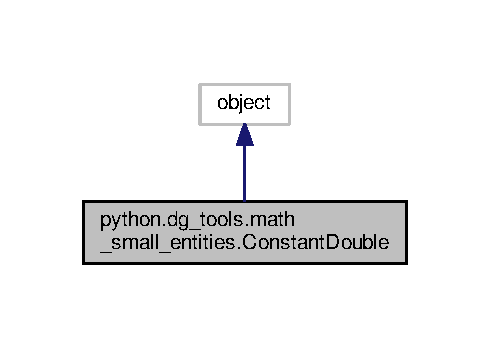
\includegraphics[width=235pt]{classpython_1_1dg__tools_1_1math__small__entities_1_1ConstantDouble__inherit__graph}
\end{center}
\end{figure}


Collaboration diagram for python.\+dg\+\_\+tools.\+math\+\_\+small\+\_\+entities.\+Constant\+Double\+:
\nopagebreak
\begin{figure}[H]
\begin{center}
\leavevmode
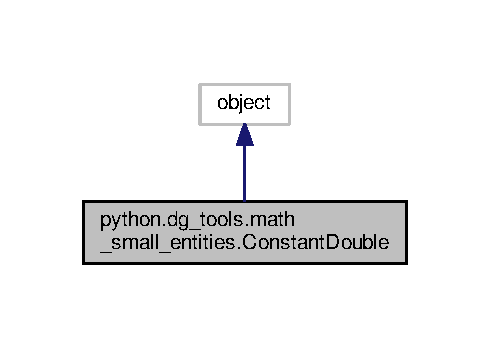
\includegraphics[width=235pt]{classpython_1_1dg__tools_1_1math__small__entities_1_1ConstantDouble__coll__graph}
\end{center}
\end{figure}
\subsection*{Public Member Functions}
\begin{DoxyCompactItemize}
\item 
def {\bfseries \+\_\+\+\_\+init\+\_\+\+\_\+} (self, value, entity\+\_\+name=\char`\"{}\char`\"{})\hypertarget{classpython_1_1dg__tools_1_1math__small__entities_1_1ConstantDouble_a5d388505a4ace7522760097798b0ffa4}{}\label{classpython_1_1dg__tools_1_1math__small__entities_1_1ConstantDouble_a5d388505a4ace7522760097798b0ffa4}

\item 
def {\bfseries set\+\_\+value} (self, value)\hypertarget{classpython_1_1dg__tools_1_1math__small__entities_1_1ConstantDouble_ae91e57cafbcddd9a9da672d58d734aa6}{}\label{classpython_1_1dg__tools_1_1math__small__entities_1_1ConstantDouble_ae91e57cafbcddd9a9da672d58d734aa6}

\item 
def {\bfseries get\+\_\+value} (self)\hypertarget{classpython_1_1dg__tools_1_1math__small__entities_1_1ConstantDouble_ad766b445d2f343cabd58827573d53225}{}\label{classpython_1_1dg__tools_1_1math__small__entities_1_1ConstantDouble_ad766b445d2f343cabd58827573d53225}

\end{DoxyCompactItemize}
\subsection*{Public Attributes}
\begin{DoxyCompactItemize}
\item 
{\bfseries add}\hypertarget{classpython_1_1dg__tools_1_1math__small__entities_1_1ConstantDouble_a05a3ff952b97d1e86ee08e6dae3b343a}{}\label{classpython_1_1dg__tools_1_1math__small__entities_1_1ConstantDouble_a05a3ff952b97d1e86ee08e6dae3b343a}

\item 
{\bfseries sin}\hypertarget{classpython_1_1dg__tools_1_1math__small__entities_1_1ConstantDouble_a151f45becbbe8644ec18506e38fcd7a0}{}\label{classpython_1_1dg__tools_1_1math__small__entities_1_1ConstantDouble_a151f45becbbe8644ec18506e38fcd7a0}

\item 
{\bfseries sout}\hypertarget{classpython_1_1dg__tools_1_1math__small__entities_1_1ConstantDouble_a0ba1911ca1603e79bfef8b6c077158be}{}\label{classpython_1_1dg__tools_1_1math__small__entities_1_1ConstantDouble_a0ba1911ca1603e79bfef8b6c077158be}

\end{DoxyCompactItemize}


\subsection{Detailed Description}
Fake an entity which provide a constant double. 

The idea is to create a \char`\"{}sout = sin1 + 0.\+0\char`\"{}, hence a constant double 

The documentation for this class was generated from the following file\+:\begin{DoxyCompactItemize}
\item 
python/dg\+\_\+tools/math\+\_\+small\+\_\+entities.\+py\end{DoxyCompactItemize}

\hypertarget{classpython_1_1dg__tools_1_1math__small__entities_1_1ConstantVector}{}\section{python.\+dg\+\_\+tools.\+math\+\_\+small\+\_\+entities.\+Constant\+Vector Class Reference}
\label{classpython_1_1dg__tools_1_1math__small__entities_1_1ConstantVector}\index{python.\+dg\+\_\+tools.\+math\+\_\+small\+\_\+entities.\+Constant\+Vector@{python.\+dg\+\_\+tools.\+math\+\_\+small\+\_\+entities.\+Constant\+Vector}}


Define a nice interface to create constant vector.  




Inheritance diagram for python.\+dg\+\_\+tools.\+math\+\_\+small\+\_\+entities.\+Constant\+Vector\+:
\nopagebreak
\begin{figure}[H]
\begin{center}
\leavevmode
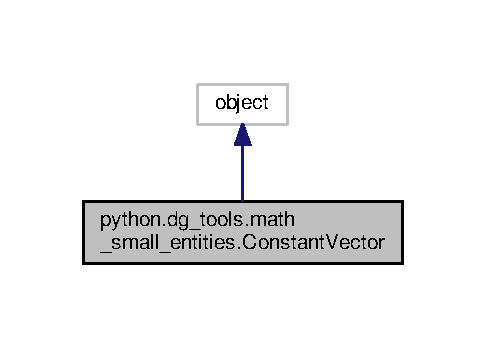
\includegraphics[width=233pt]{classpython_1_1dg__tools_1_1math__small__entities_1_1ConstantVector__inherit__graph}
\end{center}
\end{figure}


Collaboration diagram for python.\+dg\+\_\+tools.\+math\+\_\+small\+\_\+entities.\+Constant\+Vector\+:
\nopagebreak
\begin{figure}[H]
\begin{center}
\leavevmode
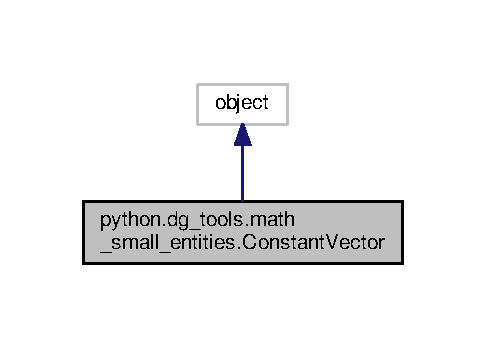
\includegraphics[width=233pt]{classpython_1_1dg__tools_1_1math__small__entities_1_1ConstantVector__coll__graph}
\end{center}
\end{figure}
\subsection*{Public Member Functions}
\begin{DoxyCompactItemize}
\item 
def {\bfseries \+\_\+\+\_\+init\+\_\+\+\_\+} (self, vec, entity\+\_\+name)\hypertarget{classpython_1_1dg__tools_1_1math__small__entities_1_1ConstantVector_ae06311463a671fb82d7172d26943da37}{}\label{classpython_1_1dg__tools_1_1math__small__entities_1_1ConstantVector_ae06311463a671fb82d7172d26943da37}

\item 
def {\bfseries set\+\_\+vec} (self, vec)\hypertarget{classpython_1_1dg__tools_1_1math__small__entities_1_1ConstantVector_a584f02de2615a0265e56ba489b4df335}{}\label{classpython_1_1dg__tools_1_1math__small__entities_1_1ConstantVector_a584f02de2615a0265e56ba489b4df335}

\item 
def {\bfseries get\+\_\+vec} (self)\hypertarget{classpython_1_1dg__tools_1_1math__small__entities_1_1ConstantVector_a551e44e0f03aa4283783d9694aac973e}{}\label{classpython_1_1dg__tools_1_1math__small__entities_1_1ConstantVector_a551e44e0f03aa4283783d9694aac973e}

\end{DoxyCompactItemize}
\subsection*{Public Attributes}
\begin{DoxyCompactItemize}
\item 
{\bfseries vec}\hypertarget{classpython_1_1dg__tools_1_1math__small__entities_1_1ConstantVector_a4a8d243668df79c77799583641991fae}{}\label{classpython_1_1dg__tools_1_1math__small__entities_1_1ConstantVector_a4a8d243668df79c77799583641991fae}

\item 
{\bfseries sout}\hypertarget{classpython_1_1dg__tools_1_1math__small__entities_1_1ConstantVector_a8b292e537665662d7697d2d9e572ece1}{}\label{classpython_1_1dg__tools_1_1math__small__entities_1_1ConstantVector_a8b292e537665662d7697d2d9e572ece1}

\end{DoxyCompactItemize}


\subsection{Detailed Description}
Define a nice interface to create constant vector. 

The documentation for this class was generated from the following file\+:\begin{DoxyCompactItemize}
\item 
python/dg\+\_\+tools/math\+\_\+small\+\_\+entities.\+py\end{DoxyCompactItemize}

\hypertarget{classdg__tools_1_1Division__of__double}{}\section{dg\+\_\+tools\+:\+:Division\+\_\+of\+\_\+double Class Reference}
\label{classdg__tools_1_1Division__of__double}\index{dg\+\_\+tools\+::\+Division\+\_\+of\+\_\+double@{dg\+\_\+tools\+::\+Division\+\_\+of\+\_\+double}}


Given input data sin1 and sin2, compute y = sin1/sin2.  




{\ttfamily \#include $<$operator.\+hpp$>$}



Inheritance diagram for dg\+\_\+tools\+:\+:Division\+\_\+of\+\_\+double\+:
\nopagebreak
\begin{figure}[H]
\begin{center}
\leavevmode
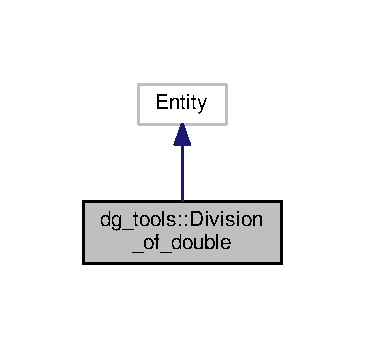
\includegraphics[width=175pt]{classdg__tools_1_1Division__of__double__inherit__graph}
\end{center}
\end{figure}


Collaboration diagram for dg\+\_\+tools\+:\+:Division\+\_\+of\+\_\+double\+:
\nopagebreak
\begin{figure}[H]
\begin{center}
\leavevmode
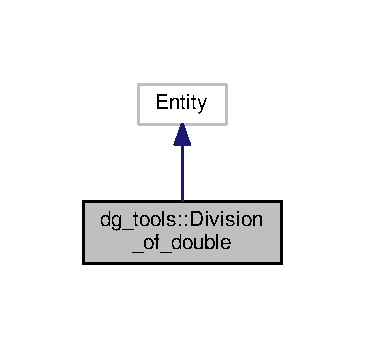
\includegraphics[width=175pt]{classdg__tools_1_1Division__of__double__coll__graph}
\end{center}
\end{figure}
\subsection*{Public Member Functions}
\begin{DoxyCompactItemize}
\item 
{\bfseries Division\+\_\+of\+\_\+double} (const std\+::string \&name)\hypertarget{classdg__tools_1_1Division__of__double_ae698007fb4d82e24174910c5385cb44c}{}\label{classdg__tools_1_1Division__of__double_ae698007fb4d82e24174910c5385cb44c}

\item 
virtual const std\+::string \& {\bfseries get\+Class\+Name} (void) const \hypertarget{classdg__tools_1_1Division__of__double_ab90859b031e0932c31a7baaef4ae7b9c}{}\label{classdg__tools_1_1Division__of__double_ab90859b031e0932c31a7baaef4ae7b9c}

\item 
double \& {\bfseries data\+\_\+out\+\_\+callback} (double \&history, int time)\hypertarget{classdg__tools_1_1Division__of__double_a40b74e93432b90ec3a4e4f6c74e326a4}{}\label{classdg__tools_1_1Division__of__double_a40b74e93432b90ec3a4e4f6c74e326a4}

\end{DoxyCompactItemize}
\subsection*{Public Attributes}
\begin{DoxyCompactItemize}
\item 
dg\+::\+Signal\+Ptr$<$ double, int $>$ {\bfseries data\+\_\+input1\+S\+IN}\hypertarget{classdg__tools_1_1Division__of__double_aaf6e1589451cddb810b38a08bd748efa}{}\label{classdg__tools_1_1Division__of__double_aaf6e1589451cddb810b38a08bd748efa}

\item 
dg\+::\+Signal\+Ptr$<$ double, int $>$ {\bfseries data\+\_\+input2\+S\+IN}\hypertarget{classdg__tools_1_1Division__of__double_a6f4769e743ed8dcca7435bde53d6d3fe}{}\label{classdg__tools_1_1Division__of__double_a6f4769e743ed8dcca7435bde53d6d3fe}

\item 
dg\+::\+Signal\+Time\+Dependent$<$ double, int $>$ {\bfseries data\+\_\+out\+S\+O\+UT}\hypertarget{classdg__tools_1_1Division__of__double_a006ca9e71348cf60feca0ec3137a65ec}{}\label{classdg__tools_1_1Division__of__double_a006ca9e71348cf60feca0ec3137a65ec}

\end{DoxyCompactItemize}
\subsection*{Static Public Attributes}
\begin{DoxyCompactItemize}
\item 
static const std\+::string {\bfseries C\+L\+A\+S\+S\+\_\+\+N\+A\+ME}\hypertarget{classdg__tools_1_1Division__of__double_a7b3fe3072ec59d063568504cf7ff6481}{}\label{classdg__tools_1_1Division__of__double_a7b3fe3072ec59d063568504cf7ff6481}

\end{DoxyCompactItemize}


\subsection{Detailed Description}
Given input data sin1 and sin2, compute y = sin1/sin2. 

The documentation for this class was generated from the following files\+:\begin{DoxyCompactItemize}
\item 
include/dg\+\_\+tools/operator.\+hpp\item 
src/operator.\+cpp\end{DoxyCompactItemize}

\hypertarget{classpython_1_1dg__tools_1_1utils_1_1DoubleSignal}{}\section{python.\+dg\+\_\+tools.\+utils.\+Double\+Signal Class Reference}
\label{classpython_1_1dg__tools_1_1utils_1_1DoubleSignal}\index{python.\+dg\+\_\+tools.\+utils.\+Double\+Signal@{python.\+dg\+\_\+tools.\+utils.\+Double\+Signal}}


Inheritance diagram for python.\+dg\+\_\+tools.\+utils.\+Double\+Signal\+:
\nopagebreak
\begin{figure}[H]
\begin{center}
\leavevmode
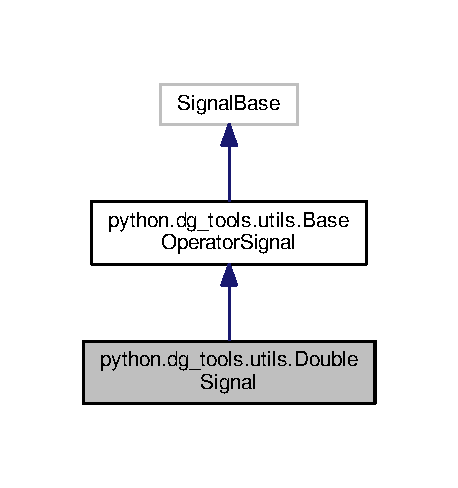
\includegraphics[width=220pt]{classpython_1_1dg__tools_1_1utils_1_1DoubleSignal__inherit__graph}
\end{center}
\end{figure}


Collaboration diagram for python.\+dg\+\_\+tools.\+utils.\+Double\+Signal\+:
\nopagebreak
\begin{figure}[H]
\begin{center}
\leavevmode
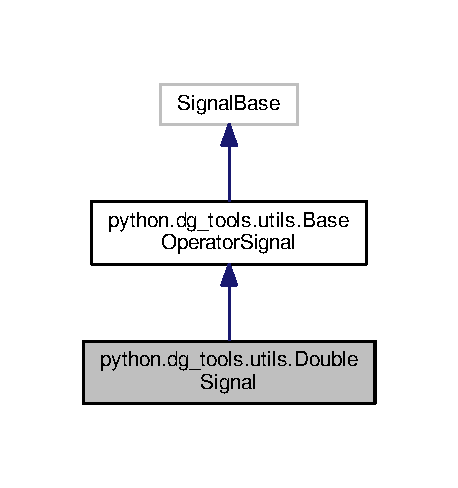
\includegraphics[width=220pt]{classpython_1_1dg__tools_1_1utils_1_1DoubleSignal__coll__graph}
\end{center}
\end{figure}
\subsection*{Public Member Functions}
\begin{DoxyCompactItemize}
\item 
def {\bfseries \+\_\+\+\_\+init\+\_\+\+\_\+} (self, sig)\hypertarget{classpython_1_1dg__tools_1_1utils_1_1DoubleSignal_ad243511463fed20c94dfe8bd540e71c5}{}\label{classpython_1_1dg__tools_1_1utils_1_1DoubleSignal_ad243511463fed20c94dfe8bd540e71c5}

\item 
def {\bfseries vector} (self)\hypertarget{classpython_1_1dg__tools_1_1utils_1_1DoubleSignal_a02d314619075a78962edcb8a2901fbdd}{}\label{classpython_1_1dg__tools_1_1utils_1_1DoubleSignal_a02d314619075a78962edcb8a2901fbdd}

\end{DoxyCompactItemize}
\subsection*{Private Attributes}
\begin{DoxyCompactItemize}
\item 
{\bfseries \+\_\+add}\hypertarget{classpython_1_1dg__tools_1_1utils_1_1DoubleSignal_ac1d0543ec22d2d0c77c0e649ddff51fa}{}\label{classpython_1_1dg__tools_1_1utils_1_1DoubleSignal_ac1d0543ec22d2d0c77c0e649ddff51fa}

\item 
{\bfseries \+\_\+sub}\hypertarget{classpython_1_1dg__tools_1_1utils_1_1DoubleSignal_a3be3dbf0972f431f8061121d87f24016}{}\label{classpython_1_1dg__tools_1_1utils_1_1DoubleSignal_a3be3dbf0972f431f8061121d87f24016}

\item 
{\bfseries \+\_\+mul}\hypertarget{classpython_1_1dg__tools_1_1utils_1_1DoubleSignal_a61864eb195e63e9c896c4ebafa24625c}{}\label{classpython_1_1dg__tools_1_1utils_1_1DoubleSignal_a61864eb195e63e9c896c4ebafa24625c}

\item 
{\bfseries \+\_\+truediv}\hypertarget{classpython_1_1dg__tools_1_1utils_1_1DoubleSignal_a7b4c19d2b4c00b18f6674951f8750655}{}\label{classpython_1_1dg__tools_1_1utils_1_1DoubleSignal_a7b4c19d2b4c00b18f6674951f8750655}

\end{DoxyCompactItemize}


The documentation for this class was generated from the following file\+:\begin{DoxyCompactItemize}
\item 
python/dg\+\_\+tools/utils.\+py\end{DoxyCompactItemize}

\hypertarget{classdg__tools_1_1HistoryRecorder}{}\section{dg\+\_\+tools\+:\+:History\+Recorder Class Reference}
\label{classdg__tools_1_1HistoryRecorder}\index{dg\+\_\+tools\+::\+History\+Recorder@{dg\+\_\+tools\+::\+History\+Recorder}}


Records data over a fixed history and yields the data as truncated vector.  




{\ttfamily \#include $<$history\+\_\+recorder.\+hpp$>$}



Inheritance diagram for dg\+\_\+tools\+:\+:History\+Recorder\+:
\nopagebreak
\begin{figure}[H]
\begin{center}
\leavevmode
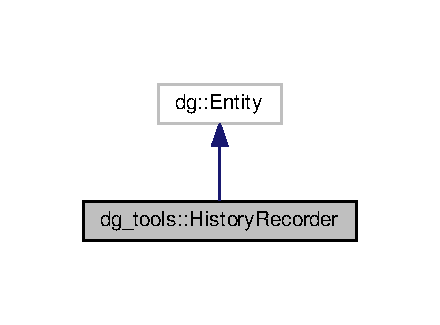
\includegraphics[width=211pt]{classdg__tools_1_1HistoryRecorder__inherit__graph}
\end{center}
\end{figure}


Collaboration diagram for dg\+\_\+tools\+:\+:History\+Recorder\+:
\nopagebreak
\begin{figure}[H]
\begin{center}
\leavevmode
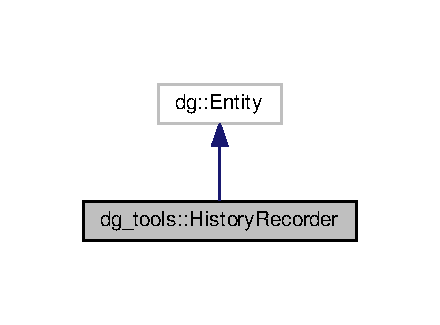
\includegraphics[width=211pt]{classdg__tools_1_1HistoryRecorder__coll__graph}
\end{center}
\end{figure}
\subsection*{Public Member Functions}
\begin{DoxyCompactItemize}
\item 
{\bfseries History\+Recorder} (const std\+::string \&name)\hypertarget{classdg__tools_1_1HistoryRecorder_a6721706c9e6a34f970ce7632193d62bd}{}\label{classdg__tools_1_1HistoryRecorder_a6721706c9e6a34f970ce7632193d62bd}

\item 
void {\bfseries init} (const int \&history\+\_\+length)\hypertarget{classdg__tools_1_1HistoryRecorder_a6343e775716b1a277f3b35a1ea0c0252}{}\label{classdg__tools_1_1HistoryRecorder_a6343e775716b1a277f3b35a1ea0c0252}

\item 
virtual void {\bfseries display} (std\+::ostream \&os) const \hypertarget{classdg__tools_1_1HistoryRecorder_af6f1a11dfc70d030eeb13dc0b8e292d7}{}\label{classdg__tools_1_1HistoryRecorder_af6f1a11dfc70d030eeb13dc0b8e292d7}

\item 
virtual const std\+::string \& {\bfseries get\+Class\+Name} (void) const \hypertarget{classdg__tools_1_1HistoryRecorder_a2cacf7271a0531080165f25f31641d51}{}\label{classdg__tools_1_1HistoryRecorder_a2cacf7271a0531080165f25f31641d51}

\item 
dg\+::\+Vector \& {\bfseries get\+History} (dg\+::\+Vector \&history, int time)\hypertarget{classdg__tools_1_1HistoryRecorder_a323b9c4f6486c03fb0914871c96aeab6}{}\label{classdg__tools_1_1HistoryRecorder_a323b9c4f6486c03fb0914871c96aeab6}

\end{DoxyCompactItemize}
\subsection*{Public Attributes}
\begin{DoxyCompactItemize}
\item 
dg\+::\+Signal\+Ptr$<$ dg\+::\+Vector, int $>$ {\bfseries data\+S\+IN}\hypertarget{classdg__tools_1_1HistoryRecorder_a8b1355d794b870d23284745069065e97}{}\label{classdg__tools_1_1HistoryRecorder_a8b1355d794b870d23284745069065e97}

\item 
dg\+::\+Signal\+Time\+Dependent$<$ dg\+::\+Vector, int $>$ {\bfseries history\+S\+O\+UT}\hypertarget{classdg__tools_1_1HistoryRecorder_ab095d5c703884e65d6232c0ca3a9ab15}{}\label{classdg__tools_1_1HistoryRecorder_ab095d5c703884e65d6232c0ca3a9ab15}

\end{DoxyCompactItemize}
\subsection*{Static Public Attributes}
\begin{DoxyCompactItemize}
\item 
static const std\+::string {\bfseries C\+L\+A\+S\+S\+\_\+\+N\+A\+ME}\hypertarget{classdg__tools_1_1HistoryRecorder_a490b6fb59e2fa5957466a4a78ca619dd}{}\label{classdg__tools_1_1HistoryRecorder_a490b6fb59e2fa5957466a4a78ca619dd}

\end{DoxyCompactItemize}
\subsection*{Private Attributes}
\begin{DoxyCompactItemize}
\item 
int {\bfseries history\+\_\+length\+\_\+}\hypertarget{classdg__tools_1_1HistoryRecorder_a210504be4f47b6663905abf4ea371f0a}{}\label{classdg__tools_1_1HistoryRecorder_a210504be4f47b6663905abf4ea371f0a}

\item 
bool {\bfseries is\+\_\+initialized\+\_\+}\hypertarget{classdg__tools_1_1HistoryRecorder_ae328c1c110447c822ba44fd90d90ae96}{}\label{classdg__tools_1_1HistoryRecorder_ae328c1c110447c822ba44fd90d90ae96}

\item 
dg\+::\+Matrix {\bfseries internal\+\_\+history\+\_\+}\hypertarget{classdg__tools_1_1HistoryRecorder_af2c34bb0fd019ac233305c61eb506476}{}\label{classdg__tools_1_1HistoryRecorder_af2c34bb0fd019ac233305c61eb506476}

\end{DoxyCompactItemize}


\subsection{Detailed Description}
Records data over a fixed history and yields the data as truncated vector. 

The newest entry is at the last position of the data array,

history = \mbox{[}data\+\_\+\{t-\/n\}, data\+\_\+\{t-\/n+1\}, ..., data\+\_\+\{t-\/1\}, data\+\_\+\{t\}\mbox{]} 

The documentation for this class was generated from the following files\+:\begin{DoxyCompactItemize}
\item 
include/dg\+\_\+tools/data/history\+\_\+recorder.\+hpp\item 
src/data/history\+\_\+recorder.\+cpp\end{DoxyCompactItemize}

\hypertarget{classpython_1_1dg__tools_1_1leg__impedance__control_1_1leg__impedance__controller_1_1LegImpedanceController}{}\section{python.\+dg\+\_\+tools.\+leg\+\_\+impedance\+\_\+control.\+leg\+\_\+impedance\+\_\+controller.\+Leg\+Impedance\+Controller Class Reference}
\label{classpython_1_1dg__tools_1_1leg__impedance__control_1_1leg__impedance__controller_1_1LegImpedanceController}\index{python.\+dg\+\_\+tools.\+leg\+\_\+impedance\+\_\+control.\+leg\+\_\+impedance\+\_\+controller.\+Leg\+Impedance\+Controller@{python.\+dg\+\_\+tools.\+leg\+\_\+impedance\+\_\+control.\+leg\+\_\+impedance\+\_\+controller.\+Leg\+Impedance\+Controller}}
\subsection*{Public Member Functions}
\begin{DoxyCompactItemize}
\item 
def {\bfseries \+\_\+\+\_\+init\+\_\+\+\_\+} (self, leg\+\_\+name)\hypertarget{classpython_1_1dg__tools_1_1leg__impedance__control_1_1leg__impedance__controller_1_1LegImpedanceController_aa1f7e3fce960dff540365c565f84a812}{}\label{classpython_1_1dg__tools_1_1leg__impedance__control_1_1leg__impedance__controller_1_1LegImpedanceController_aa1f7e3fce960dff540365c565f84a812}

\item 
def \hyperlink{classpython_1_1dg__tools_1_1leg__impedance__control_1_1leg__impedance__controller_1_1LegImpedanceController_a4c88fb5d9e5a89c4cb1df9198475bda9}{return\+\_\+leg\+\_\+length} (self)\hypertarget{classpython_1_1dg__tools_1_1leg__impedance__control_1_1leg__impedance__controller_1_1LegImpedanceController_a4c88fb5d9e5a89c4cb1df9198475bda9}{}\label{classpython_1_1dg__tools_1_1leg__impedance__control_1_1leg__impedance__controller_1_1LegImpedanceController_a4c88fb5d9e5a89c4cb1df9198475bda9}

\begin{DoxyCompactList}\small\item\em \paragraph*{Computes current leg length}\end{DoxyCompactList}\item 
def {\bfseries return\+\_\+control\+\_\+torques} (self, kp, des\+\_\+pos, kd=None, des\+\_\+vel=None, kf=None, fff=None)\hypertarget{classpython_1_1dg__tools_1_1leg__impedance__control_1_1leg__impedance__controller_1_1LegImpedanceController_a2560dfe16255f843fec19f1492f34bc1}{}\label{classpython_1_1dg__tools_1_1leg__impedance__control_1_1leg__impedance__controller_1_1LegImpedanceController_a2560dfe16255f843fec19f1492f34bc1}

\item 
def {\bfseries record\+\_\+data} (self, robot)\hypertarget{classpython_1_1dg__tools_1_1leg__impedance__control_1_1leg__impedance__controller_1_1LegImpedanceController_a51fbd868010ad4a475fbc38b2c37a032}{}\label{classpython_1_1dg__tools_1_1leg__impedance__control_1_1leg__impedance__controller_1_1LegImpedanceController_a51fbd868010ad4a475fbc38b2c37a032}

\end{DoxyCompactItemize}
\subsection*{Public Attributes}
\begin{DoxyCompactItemize}
\item 
{\bfseries leg\+\_\+name}\hypertarget{classpython_1_1dg__tools_1_1leg__impedance__control_1_1leg__impedance__controller_1_1LegImpedanceController_a8094365ea991d0c5d1f54d8ff75bff86}{}\label{classpython_1_1dg__tools_1_1leg__impedance__control_1_1leg__impedance__controller_1_1LegImpedanceController_a8094365ea991d0c5d1f54d8ff75bff86}

\item 
{\bfseries robot\+\_\+pin}\hypertarget{classpython_1_1dg__tools_1_1leg__impedance__control_1_1leg__impedance__controller_1_1LegImpedanceController_a3a887b72be4a41ba4cab4457fd935e90}{}\label{classpython_1_1dg__tools_1_1leg__impedance__control_1_1leg__impedance__controller_1_1LegImpedanceController_a3a887b72be4a41ba4cab4457fd935e90}

\item 
{\bfseries robot\+\_\+dg}\hypertarget{classpython_1_1dg__tools_1_1leg__impedance__control_1_1leg__impedance__controller_1_1LegImpedanceController_aa8cf0226bf2c1583ad3edc4079fa6bfb}{}\label{classpython_1_1dg__tools_1_1leg__impedance__control_1_1leg__impedance__controller_1_1LegImpedanceController_aa8cf0226bf2c1583ad3edc4079fa6bfb}

\item 
{\bfseries joint\+\_\+positions\+\_\+sin}\hypertarget{classpython_1_1dg__tools_1_1leg__impedance__control_1_1leg__impedance__controller_1_1LegImpedanceController_a2d97fcd05ed8588b59b6a71d03374f77}{}\label{classpython_1_1dg__tools_1_1leg__impedance__control_1_1leg__impedance__controller_1_1LegImpedanceController_a2d97fcd05ed8588b59b6a71d03374f77}

\item 
{\bfseries joint\+\_\+velocities\+\_\+sin}\hypertarget{classpython_1_1dg__tools_1_1leg__impedance__control_1_1leg__impedance__controller_1_1LegImpedanceController_a381159ee8e5924469b8912e9b3213fd2}{}\label{classpython_1_1dg__tools_1_1leg__impedance__control_1_1leg__impedance__controller_1_1LegImpedanceController_a381159ee8e5924469b8912e9b3213fd2}

\item 
{\bfseries xyzpos\+\_\+hip}\hypertarget{classpython_1_1dg__tools_1_1leg__impedance__control_1_1leg__impedance__controller_1_1LegImpedanceController_ad8c5846d949a1e14cd91255e96d9161c}{}\label{classpython_1_1dg__tools_1_1leg__impedance__control_1_1leg__impedance__controller_1_1LegImpedanceController_ad8c5846d949a1e14cd91255e96d9161c}

\item 
{\bfseries xyzpos\+\_\+foot}\hypertarget{classpython_1_1dg__tools_1_1leg__impedance__control_1_1leg__impedance__controller_1_1LegImpedanceController_ae2d266ce60200f5c3d4a273863e444bb}{}\label{classpython_1_1dg__tools_1_1leg__impedance__control_1_1leg__impedance__controller_1_1LegImpedanceController_ae2d266ce60200f5c3d4a273863e444bb}

\item 
{\bfseries rel\+\_\+pos\+\_\+foot}\hypertarget{classpython_1_1dg__tools_1_1leg__impedance__control_1_1leg__impedance__controller_1_1LegImpedanceController_afe97a475184a29f5f43092afcd01d673}{}\label{classpython_1_1dg__tools_1_1leg__impedance__control_1_1leg__impedance__controller_1_1LegImpedanceController_afe97a475184a29f5f43092afcd01d673}

\item 
{\bfseries rct\+\_\+args}\hypertarget{classpython_1_1dg__tools_1_1leg__impedance__control_1_1leg__impedance__controller_1_1LegImpedanceController_ad8b54c7826ccaba33e7bb99e13b1e177}{}\label{classpython_1_1dg__tools_1_1leg__impedance__control_1_1leg__impedance__controller_1_1LegImpedanceController_ad8b54c7826ccaba33e7bb99e13b1e177}

\item 
{\bfseries jac}\hypertarget{classpython_1_1dg__tools_1_1leg__impedance__control_1_1leg__impedance__controller_1_1LegImpedanceController_a0e30827957a254793f36cc9b619f8c41}{}\label{classpython_1_1dg__tools_1_1leg__impedance__control_1_1leg__impedance__controller_1_1LegImpedanceController_a0e30827957a254793f36cc9b619f8c41}

\item 
{\bfseries pos\+\_\+error}\hypertarget{classpython_1_1dg__tools_1_1leg__impedance__control_1_1leg__impedance__controller_1_1LegImpedanceController_a8f54abb271f0fb18516871c454ead08b}{}\label{classpython_1_1dg__tools_1_1leg__impedance__control_1_1leg__impedance__controller_1_1LegImpedanceController_a8f54abb271f0fb18516871c454ead08b}

\item 
{\bfseries rel\+\_\+vel\+\_\+foot}\hypertarget{classpython_1_1dg__tools_1_1leg__impedance__control_1_1leg__impedance__controller_1_1LegImpedanceController_ad8d7dd70797a5c9190b2454a51d3312a}{}\label{classpython_1_1dg__tools_1_1leg__impedance__control_1_1leg__impedance__controller_1_1LegImpedanceController_ad8d7dd70797a5c9190b2454a51d3312a}

\item 
{\bfseries vel\+\_\+error}\hypertarget{classpython_1_1dg__tools_1_1leg__impedance__control_1_1leg__impedance__controller_1_1LegImpedanceController_ae7c6a380c196ceeedd7e5067c8995600}{}\label{classpython_1_1dg__tools_1_1leg__impedance__control_1_1leg__impedance__controller_1_1LegImpedanceController_ae7c6a380c196ceeedd7e5067c8995600}

\item 
{\bfseries pd\+\_\+error}\hypertarget{classpython_1_1dg__tools_1_1leg__impedance__control_1_1leg__impedance__controller_1_1LegImpedanceController_ac084d227c1362c85e910196812864ec4}{}\label{classpython_1_1dg__tools_1_1leg__impedance__control_1_1leg__impedance__controller_1_1LegImpedanceController_ac084d227c1362c85e910196812864ec4}

\item 
{\bfseries total\+\_\+error}\hypertarget{classpython_1_1dg__tools_1_1leg__impedance__control_1_1leg__impedance__controller_1_1LegImpedanceController_acb3c2792b4b35c6b7606023adbc09001}{}\label{classpython_1_1dg__tools_1_1leg__impedance__control_1_1leg__impedance__controller_1_1LegImpedanceController_acb3c2792b4b35c6b7606023adbc09001}

\item 
{\bfseries estimated\+\_\+foot\+\_\+force}\hypertarget{classpython_1_1dg__tools_1_1leg__impedance__control_1_1leg__impedance__controller_1_1LegImpedanceController_ac02390fb0ab1a6c9c4fb3a02bb8443bc}{}\label{classpython_1_1dg__tools_1_1leg__impedance__control_1_1leg__impedance__controller_1_1LegImpedanceController_ac02390fb0ab1a6c9c4fb3a02bb8443bc}

\end{DoxyCompactItemize}
\subsection*{Private Member Functions}
\begin{DoxyCompactItemize}
\item 
def {\bfseries \+\_\+compute\+\_\+control\+\_\+torques} (self, start\+\_\+index=1, end\+\_\+index=3)\hypertarget{classpython_1_1dg__tools_1_1leg__impedance__control_1_1leg__impedance__controller_1_1LegImpedanceController_ac7abf513267b2626ce9fd191a7d7e061}{}\label{classpython_1_1dg__tools_1_1leg__impedance__control_1_1leg__impedance__controller_1_1LegImpedanceController_ac7abf513267b2626ce9fd191a7d7e061}

\end{DoxyCompactItemize}


The documentation for this class was generated from the following file\+:\begin{DoxyCompactItemize}
\item 
python/dg\+\_\+tools/leg\+\_\+impedance\+\_\+control/\hyperlink{leg__impedance__controller_8py}{leg\+\_\+impedance\+\_\+controller.\+py}\end{DoxyCompactItemize}

\hypertarget{classdg__tools_1_1MemoryReplay}{}\section{dg\+\_\+tools\+:\+:Memory\+Replay Class Reference}
\label{classdg__tools_1_1MemoryReplay}\index{dg\+\_\+tools\+::\+Memory\+Replay@{dg\+\_\+tools\+::\+Memory\+Replay}}


Provided with a matrix, the entity returns the row indexed by the current time index at every timestep.  




{\ttfamily \#include $<$memory\+\_\+replay.\+hpp$>$}



Inheritance diagram for dg\+\_\+tools\+:\+:Memory\+Replay\+:
\nopagebreak
\begin{figure}[H]
\begin{center}
\leavevmode
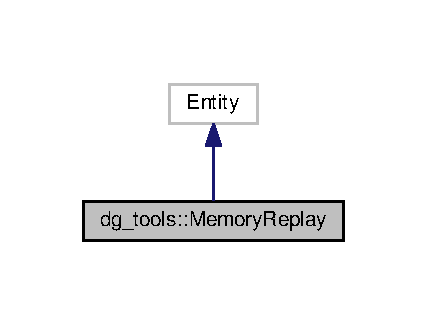
\includegraphics[width=205pt]{classdg__tools_1_1MemoryReplay__inherit__graph}
\end{center}
\end{figure}


Collaboration diagram for dg\+\_\+tools\+:\+:Memory\+Replay\+:
\nopagebreak
\begin{figure}[H]
\begin{center}
\leavevmode
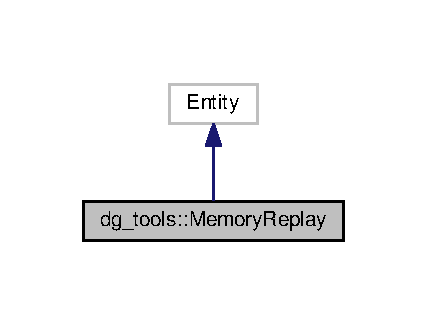
\includegraphics[width=205pt]{classdg__tools_1_1MemoryReplay__coll__graph}
\end{center}
\end{figure}
\subsection*{Public Member Functions}
\begin{DoxyCompactItemize}
\item 
{\bfseries Memory\+Replay} (const std\+::string \&name)\hypertarget{classdg__tools_1_1MemoryReplay_a8337a556eae14b1f8259487c0ab79b31}{}\label{classdg__tools_1_1MemoryReplay_a8337a556eae14b1f8259487c0ab79b31}

\item 
void {\bfseries init} (const dg\+::\+Matrix \&data)\hypertarget{classdg__tools_1_1MemoryReplay_a6fabc46d90fc14020e3122638528a3c4}{}\label{classdg__tools_1_1MemoryReplay_a6fabc46d90fc14020e3122638528a3c4}

\item 
void {\bfseries rewind} ()\hypertarget{classdg__tools_1_1MemoryReplay_a659c4c6d6a053d4a62ddd3593dba2c23}{}\label{classdg__tools_1_1MemoryReplay_a659c4c6d6a053d4a62ddd3593dba2c23}

\item 
virtual const std\+::string \& {\bfseries get\+Class\+Name} (void) const \hypertarget{classdg__tools_1_1MemoryReplay_a0bb7c62a85661716411924aa0a9dad51}{}\label{classdg__tools_1_1MemoryReplay_a0bb7c62a85661716411924aa0a9dad51}

\item 
dg\+::\+Vector \& {\bfseries get\+Value} (dg\+::\+Vector \&sout, int time)\hypertarget{classdg__tools_1_1MemoryReplay_a8ab59d0192c29bc4701171276f8d3e67}{}\label{classdg__tools_1_1MemoryReplay_a8ab59d0192c29bc4701171276f8d3e67}

\end{DoxyCompactItemize}
\subsection*{Public Attributes}
\begin{DoxyCompactItemize}
\item 
dg\+::\+Signal\+Time\+Dependent$<$ dg\+::\+Vector, int $>$ {\bfseries internal\+\_\+signal\+\_\+refresher\+\_\+}\hypertarget{classdg__tools_1_1MemoryReplay_a2d096c1d9ab01da6af070141de32a1ad}{}\label{classdg__tools_1_1MemoryReplay_a2d096c1d9ab01da6af070141de32a1ad}

\item 
dg\+::\+Signal\+Time\+Dependent$<$ dg\+::\+Vector, int $>$ {\bfseries sout}\hypertarget{classdg__tools_1_1MemoryReplay_a2a7e1605201f102754dbb9d79b14a79d}{}\label{classdg__tools_1_1MemoryReplay_a2a7e1605201f102754dbb9d79b14a79d}

\end{DoxyCompactItemize}
\subsection*{Static Public Attributes}
\begin{DoxyCompactItemize}
\item 
static const std\+::string {\bfseries C\+L\+A\+S\+S\+\_\+\+N\+A\+ME}\hypertarget{classdg__tools_1_1MemoryReplay_a99b1ae11beccebec65c26e38b670366e}{}\label{classdg__tools_1_1MemoryReplay_a99b1ae11beccebec65c26e38b670366e}

\end{DoxyCompactItemize}
\subsection*{Private Attributes}
\begin{DoxyCompactItemize}
\item 
bool {\bfseries is\+\_\+started\+\_\+}\hypertarget{classdg__tools_1_1MemoryReplay_a878349c497242a2dbe9ef0314fc22cf7}{}\label{classdg__tools_1_1MemoryReplay_a878349c497242a2dbe9ef0314fc22cf7}

\item 
int {\bfseries start\+\_\+time\+\_\+}\hypertarget{classdg__tools_1_1MemoryReplay_a7d1394b959e16997e30ee1b5f92776d3}{}\label{classdg__tools_1_1MemoryReplay_a7d1394b959e16997e30ee1b5f92776d3}

\item 
dg\+::\+Matrix {\bfseries data\+\_\+}\hypertarget{classdg__tools_1_1MemoryReplay_a690c7a438233ac381cbfafb0fb0a93da}{}\label{classdg__tools_1_1MemoryReplay_a690c7a438233ac381cbfafb0fb0a93da}

\end{DoxyCompactItemize}


\subsection{Detailed Description}
Provided with a matrix, the entity returns the row indexed by the current time index at every timestep. 

Example\+: Store a desired trajectory in memory and get the desired position at every timestep. 

The documentation for this class was generated from the following files\+:\begin{DoxyCompactItemize}
\item 
include/dg\+\_\+tools/data/memory\+\_\+replay.\+hpp\item 
src/data/memory\+\_\+replay.\+cpp\end{DoxyCompactItemize}

\hypertarget{classpython_1_1dg__tools_1_1math__small__entities_1_1MultiplyDoubleVector}{}\section{python.\+dg\+\_\+tools.\+math\+\_\+small\+\_\+entities.\+Multiply\+Double\+Vector Class Reference}
\label{classpython_1_1dg__tools_1_1math__small__entities_1_1MultiplyDoubleVector}\index{python.\+dg\+\_\+tools.\+math\+\_\+small\+\_\+entities.\+Multiply\+Double\+Vector@{python.\+dg\+\_\+tools.\+math\+\_\+small\+\_\+entities.\+Multiply\+Double\+Vector}}


Simpler interface to multiply a double and a vector.  




Inheritance diagram for python.\+dg\+\_\+tools.\+math\+\_\+small\+\_\+entities.\+Multiply\+Double\+Vector\+:
\nopagebreak
\begin{figure}[H]
\begin{center}
\leavevmode
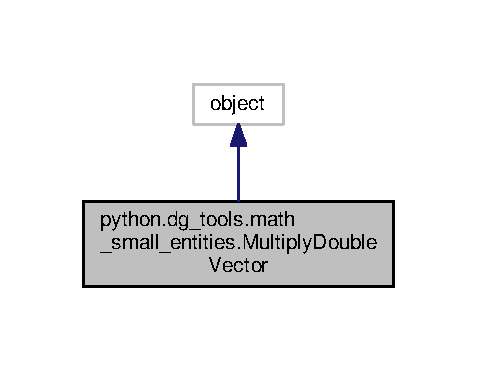
\includegraphics[width=229pt]{classpython_1_1dg__tools_1_1math__small__entities_1_1MultiplyDoubleVector__inherit__graph}
\end{center}
\end{figure}


Collaboration diagram for python.\+dg\+\_\+tools.\+math\+\_\+small\+\_\+entities.\+Multiply\+Double\+Vector\+:
\nopagebreak
\begin{figure}[H]
\begin{center}
\leavevmode
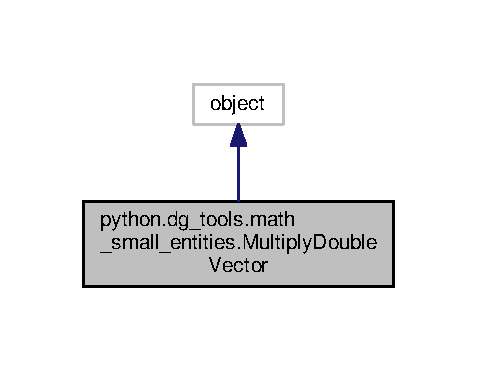
\includegraphics[width=229pt]{classpython_1_1dg__tools_1_1math__small__entities_1_1MultiplyDoubleVector__coll__graph}
\end{center}
\end{figure}
\subsection*{Public Member Functions}
\begin{DoxyCompactItemize}
\item 
def {\bfseries \+\_\+\+\_\+init\+\_\+\+\_\+} (self, double\+\_\+sin, vector\+\_\+sin, entity\+\_\+name=\textquotesingle{}\textquotesingle{})\hypertarget{classpython_1_1dg__tools_1_1math__small__entities_1_1MultiplyDoubleVector_a686fa93d5e4eb5715a0e945b7f74eebd}{}\label{classpython_1_1dg__tools_1_1math__small__entities_1_1MultiplyDoubleVector_a686fa93d5e4eb5715a0e945b7f74eebd}

\end{DoxyCompactItemize}
\subsection*{Public Attributes}
\begin{DoxyCompactItemize}
\item 
{\bfseries op}\hypertarget{classpython_1_1dg__tools_1_1math__small__entities_1_1MultiplyDoubleVector_a457e6937d9762373d4e1442ef0f8063a}{}\label{classpython_1_1dg__tools_1_1math__small__entities_1_1MultiplyDoubleVector_a457e6937d9762373d4e1442ef0f8063a}

\item 
{\bfseries sin1}\hypertarget{classpython_1_1dg__tools_1_1math__small__entities_1_1MultiplyDoubleVector_ab9af832a8c134bf03fca80168dbe757b}{}\label{classpython_1_1dg__tools_1_1math__small__entities_1_1MultiplyDoubleVector_ab9af832a8c134bf03fca80168dbe757b}

\item 
{\bfseries sin2}\hypertarget{classpython_1_1dg__tools_1_1math__small__entities_1_1MultiplyDoubleVector_aed7cf50295ab6be0381522a8bbd7a637}{}\label{classpython_1_1dg__tools_1_1math__small__entities_1_1MultiplyDoubleVector_aed7cf50295ab6be0381522a8bbd7a637}

\item 
{\bfseries sout}\hypertarget{classpython_1_1dg__tools_1_1math__small__entities_1_1MultiplyDoubleVector_ac06f0ebb1bbda12565e5d33bb634cee2}{}\label{classpython_1_1dg__tools_1_1math__small__entities_1_1MultiplyDoubleVector_ac06f0ebb1bbda12565e5d33bb634cee2}

\end{DoxyCompactItemize}


\subsection{Detailed Description}
Simpler interface to multiply a double and a vector. 

The documentation for this class was generated from the following file\+:\begin{DoxyCompactItemize}
\item 
python/dg\+\_\+tools/math\+\_\+small\+\_\+entities.\+py\end{DoxyCompactItemize}

\hypertarget{classdynamicgraph_1_1sot_1_1PDController}{}\section{dynamicgraph\+:\+:sot\+:\+:P\+D\+Controller Class Reference}
\label{classdynamicgraph_1_1sot_1_1PDController}\index{dynamicgraph\+::sot\+::\+P\+D\+Controller@{dynamicgraph\+::sot\+::\+P\+D\+Controller}}


Inheritance diagram for dynamicgraph\+:\+:sot\+:\+:P\+D\+Controller\+:
\nopagebreak
\begin{figure}[H]
\begin{center}
\leavevmode
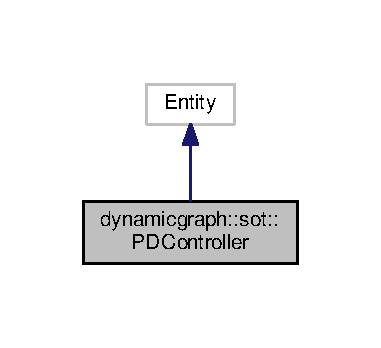
\includegraphics[width=183pt]{classdynamicgraph_1_1sot_1_1PDController__inherit__graph}
\end{center}
\end{figure}


Collaboration diagram for dynamicgraph\+:\+:sot\+:\+:P\+D\+Controller\+:
\nopagebreak
\begin{figure}[H]
\begin{center}
\leavevmode
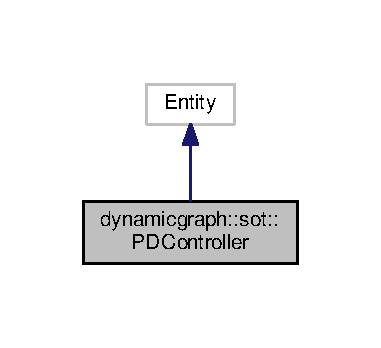
\includegraphics[width=183pt]{classdynamicgraph_1_1sot_1_1PDController__coll__graph}
\end{center}
\end{figure}
\subsection*{Public Member Functions}
\begin{DoxyCompactItemize}
\item 
{\bfseries P\+D\+Controller} (const std\+::string \&name)\hypertarget{classdynamicgraph_1_1sot_1_1PDController_a81f0b4f965c6d747d51e425bcf6b1e87}{}\label{classdynamicgraph_1_1sot_1_1PDController_a81f0b4f965c6d747d51e425bcf6b1e87}

\item 
virtual void {\bfseries display} (std\+::ostream \&os) const \hypertarget{classdynamicgraph_1_1sot_1_1PDController_a5d31b7c1fbcfe371d1de29a077687ddb}{}\label{classdynamicgraph_1_1sot_1_1PDController_a5d31b7c1fbcfe371d1de29a077687ddb}

\item 
virtual const std\+::string \& {\bfseries get\+Class\+Name} (void) const \hypertarget{classdynamicgraph_1_1sot_1_1PDController_a6026ca5af993bfa197c1a4b7b7170666}{}\label{classdynamicgraph_1_1sot_1_1PDController_a6026ca5af993bfa197c1a4b7b7170666}

\end{DoxyCompactItemize}
\subsection*{Public Attributes}
\begin{DoxyCompactItemize}
\item 
Signal\+Ptr$<$ dg\+::\+Vector, int $>$ {\bfseries Kp\+S\+IN}\hypertarget{classdynamicgraph_1_1sot_1_1PDController_ad4fc27adfdc622ff227b2df5dd9ff3e3}{}\label{classdynamicgraph_1_1sot_1_1PDController_ad4fc27adfdc622ff227b2df5dd9ff3e3}

\item 
Signal\+Ptr$<$ dg\+::\+Vector, int $>$ {\bfseries Kd\+S\+IN}\hypertarget{classdynamicgraph_1_1sot_1_1PDController_ade6af9695793655239b9df09cc013852}{}\label{classdynamicgraph_1_1sot_1_1PDController_ade6af9695793655239b9df09cc013852}

\item 
Signal\+Ptr$<$ dg\+::\+Vector, int $>$ {\bfseries position\+S\+IN}\hypertarget{classdynamicgraph_1_1sot_1_1PDController_aa28a076a093e91de78ab10ff4bf257d3}{}\label{classdynamicgraph_1_1sot_1_1PDController_aa28a076a093e91de78ab10ff4bf257d3}

\item 
Signal\+Ptr$<$ dg\+::\+Vector, int $>$ {\bfseries desiredposition\+S\+IN}\hypertarget{classdynamicgraph_1_1sot_1_1PDController_ae90d924ffaf3c4e54af32a25ddb136f1}{}\label{classdynamicgraph_1_1sot_1_1PDController_ae90d924ffaf3c4e54af32a25ddb136f1}

\item 
Signal\+Ptr$<$ dg\+::\+Vector, int $>$ {\bfseries velocity\+S\+IN}\hypertarget{classdynamicgraph_1_1sot_1_1PDController_a501c2b9b92bb5b4d4bc6ea9190b9a87e}{}\label{classdynamicgraph_1_1sot_1_1PDController_a501c2b9b92bb5b4d4bc6ea9190b9a87e}

\item 
Signal\+Ptr$<$ dg\+::\+Vector, int $>$ {\bfseries desiredvelocity\+S\+IN}\hypertarget{classdynamicgraph_1_1sot_1_1PDController_a30f38b6ea6a9ba584a4b0ccf02af925a}{}\label{classdynamicgraph_1_1sot_1_1PDController_a30f38b6ea6a9ba584a4b0ccf02af925a}

\item 
Signal\+Time\+Dependent$<$ dg\+::\+Vector, int $>$ {\bfseries control\+S\+O\+UT}\hypertarget{classdynamicgraph_1_1sot_1_1PDController_a39554a8525100823dfface5d0eb5846a}{}\label{classdynamicgraph_1_1sot_1_1PDController_a39554a8525100823dfface5d0eb5846a}

\item 
Signal\+Time\+Dependent$<$ dg\+::\+Vector, int $>$ {\bfseries position\+Error\+S\+O\+UT}\hypertarget{classdynamicgraph_1_1sot_1_1PDController_af45ff8d1a1d6c7c4c1eb18e51b0311bc}{}\label{classdynamicgraph_1_1sot_1_1PDController_af45ff8d1a1d6c7c4c1eb18e51b0311bc}

\item 
Signal\+Time\+Dependent$<$ dg\+::\+Vector, int $>$ {\bfseries velocity\+Error\+S\+O\+UT}\hypertarget{classdynamicgraph_1_1sot_1_1PDController_a91745aa2d68db845e4b27ba67b39baa9}{}\label{classdynamicgraph_1_1sot_1_1PDController_a91745aa2d68db845e4b27ba67b39baa9}

\end{DoxyCompactItemize}
\subsection*{Static Public Attributes}
\begin{DoxyCompactItemize}
\item 
static const double {\bfseries T\+I\+M\+E\+\_\+\+S\+T\+E\+P\+\_\+\+D\+E\+F\+A\+U\+LT} = .\+001\hypertarget{classdynamicgraph_1_1sot_1_1PDController_a0fd0dd695567d7daa489a5ef2a8028cf}{}\label{classdynamicgraph_1_1sot_1_1PDController_a0fd0dd695567d7daa489a5ef2a8028cf}

\item 
static const std\+::string {\bfseries C\+L\+A\+S\+S\+\_\+\+N\+A\+ME}\hypertarget{classdynamicgraph_1_1sot_1_1PDController_a2a377e6b4997e8c0123bb925a59081e7}{}\label{classdynamicgraph_1_1sot_1_1PDController_a2a377e6b4997e8c0123bb925a59081e7}

\end{DoxyCompactItemize}
\subsection*{Protected Member Functions}
\begin{DoxyCompactItemize}
\item 
double \& {\bfseries setsize} (int dimension)\hypertarget{classdynamicgraph_1_1sot_1_1PDController_a52c3f044f1fc263b3bfd6f6c3e55458d}{}\label{classdynamicgraph_1_1sot_1_1PDController_a52c3f044f1fc263b3bfd6f6c3e55458d}

\item 
dg\+::\+Vector \& {\bfseries compute\+Control} (dg\+::\+Vector \&tau, int t)\hypertarget{classdynamicgraph_1_1sot_1_1PDController_a1c1b10166419971121ec5418bf79332b}{}\label{classdynamicgraph_1_1sot_1_1PDController_a1c1b10166419971121ec5418bf79332b}

\item 
dg\+::\+Vector \& {\bfseries get\+Position\+Error} (dg\+::\+Vector \&position\+\_\+error, int t)\hypertarget{classdynamicgraph_1_1sot_1_1PDController_ad4c37478445c4556752da1d6bdfedf00}{}\label{classdynamicgraph_1_1sot_1_1PDController_ad4c37478445c4556752da1d6bdfedf00}

\item 
dg\+::\+Vector \& {\bfseries get\+Velocity\+Error} (dg\+::\+Vector \&velocity\+\_\+error, int t)\hypertarget{classdynamicgraph_1_1sot_1_1PDController_a2ec1b3f5eade54cfaa6f2c6e25f04267}{}\label{classdynamicgraph_1_1sot_1_1PDController_a2ec1b3f5eade54cfaa6f2c6e25f04267}

\end{DoxyCompactItemize}
\subsection*{Protected Attributes}
\begin{DoxyCompactItemize}
\item 
double {\bfseries Time\+Step}\hypertarget{classdynamicgraph_1_1sot_1_1PDController_a9043aaa176798471184f915d1d75d122}{}\label{classdynamicgraph_1_1sot_1_1PDController_a9043aaa176798471184f915d1d75d122}

\item 
double {\bfseries \+\_\+dimension}\hypertarget{classdynamicgraph_1_1sot_1_1PDController_ac2a7facafb80c1a41d825b2653eada59}{}\label{classdynamicgraph_1_1sot_1_1PDController_ac2a7facafb80c1a41d825b2653eada59}

\item 
dg\+::\+Vector {\bfseries position\+\_\+error}\hypertarget{classdynamicgraph_1_1sot_1_1PDController_af4779f470097a80de134de3f9e08433a}{}\label{classdynamicgraph_1_1sot_1_1PDController_af4779f470097a80de134de3f9e08433a}

\item 
dg\+::\+Vector {\bfseries velocity\+\_\+error}\hypertarget{classdynamicgraph_1_1sot_1_1PDController_ad8f0f65f4045b86d64517539580376a8}{}\label{classdynamicgraph_1_1sot_1_1PDController_ad8f0f65f4045b86d64517539580376a8}

\end{DoxyCompactItemize}


The documentation for this class was generated from the following files\+:\begin{DoxyCompactItemize}
\item 
include/dg\+\_\+tools/control/\hyperlink{control__pd_8hpp}{control\+\_\+pd.\+hpp}\item 
src/control/control\+\_\+pd.\+cpp\end{DoxyCompactItemize}

\hypertarget{classdg__tools_1_1PoseQuaternionToPoseRPY}{}\section{dg\+\_\+tools\+:\+:Pose\+Quaternion\+To\+Pose\+R\+PY Class Reference}
\label{classdg__tools_1_1PoseQuaternionToPoseRPY}\index{dg\+\_\+tools\+::\+Pose\+Quaternion\+To\+Pose\+R\+PY@{dg\+\_\+tools\+::\+Pose\+Quaternion\+To\+Pose\+R\+PY}}


Converts Pose\+Quaternion into Pose\+R\+PY data.  




{\ttfamily \#include $<$operator.\+hpp$>$}



Inheritance diagram for dg\+\_\+tools\+:\+:Pose\+Quaternion\+To\+Pose\+R\+PY\+:
\nopagebreak
\begin{figure}[H]
\begin{center}
\leavevmode
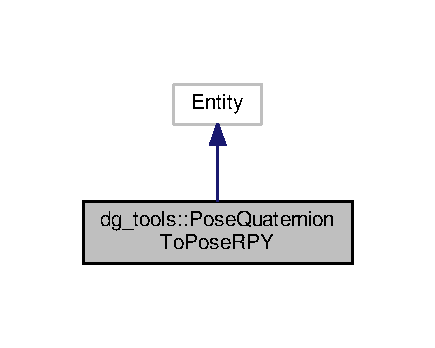
\includegraphics[width=209pt]{classdg__tools_1_1PoseQuaternionToPoseRPY__inherit__graph}
\end{center}
\end{figure}


Collaboration diagram for dg\+\_\+tools\+:\+:Pose\+Quaternion\+To\+Pose\+R\+PY\+:
\nopagebreak
\begin{figure}[H]
\begin{center}
\leavevmode
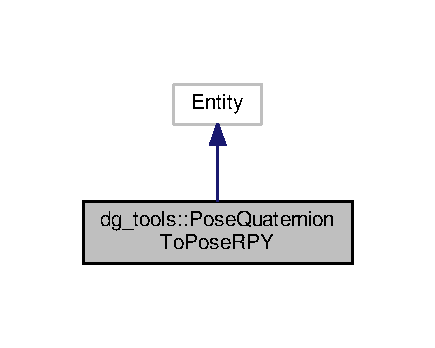
\includegraphics[width=209pt]{classdg__tools_1_1PoseQuaternionToPoseRPY__coll__graph}
\end{center}
\end{figure}
\subsection*{Public Member Functions}
\begin{DoxyCompactItemize}
\item 
{\bfseries Pose\+Quaternion\+To\+Pose\+R\+PY} (const std\+::string \&name)\hypertarget{classdg__tools_1_1PoseQuaternionToPoseRPY_a0448f85839f5548a9ce8db65a31928df}{}\label{classdg__tools_1_1PoseQuaternionToPoseRPY_a0448f85839f5548a9ce8db65a31928df}

\item 
virtual const std\+::string \& {\bfseries get\+Class\+Name} (void) const \hypertarget{classdg__tools_1_1PoseQuaternionToPoseRPY_a6add152d85612d3d5c102daa7a380a8e}{}\label{classdg__tools_1_1PoseQuaternionToPoseRPY_a6add152d85612d3d5c102daa7a380a8e}

\item 
dg\+::\+Vector \& {\bfseries data\+\_\+out\+\_\+callback} (dg\+::\+Vector \&history, int time)\hypertarget{classdg__tools_1_1PoseQuaternionToPoseRPY_a465523da36b94ef86fe20298b8984feb}{}\label{classdg__tools_1_1PoseQuaternionToPoseRPY_a465523da36b94ef86fe20298b8984feb}

\end{DoxyCompactItemize}
\subsection*{Public Attributes}
\begin{DoxyCompactItemize}
\item 
dg\+::\+Signal\+Ptr$<$ dg\+::\+Vector, int $>$ {\bfseries data\+\_\+input\+S\+IN}\hypertarget{classdg__tools_1_1PoseQuaternionToPoseRPY_ae32171988c5e9efee47e78de71c692b5}{}\label{classdg__tools_1_1PoseQuaternionToPoseRPY_ae32171988c5e9efee47e78de71c692b5}

\item 
dg\+::\+Signal\+Time\+Dependent$<$ dg\+::\+Vector, int $>$ {\bfseries data\+\_\+out\+S\+O\+UT}\hypertarget{classdg__tools_1_1PoseQuaternionToPoseRPY_a84652f7e1f7023d48418a311ed7ae42e}{}\label{classdg__tools_1_1PoseQuaternionToPoseRPY_a84652f7e1f7023d48418a311ed7ae42e}

\end{DoxyCompactItemize}
\subsection*{Static Public Attributes}
\begin{DoxyCompactItemize}
\item 
static const std\+::string {\bfseries C\+L\+A\+S\+S\+\_\+\+N\+A\+ME}\hypertarget{classdg__tools_1_1PoseQuaternionToPoseRPY_afcb55058e0af2e02f6d2ac4e8354f7a9}{}\label{classdg__tools_1_1PoseQuaternionToPoseRPY_afcb55058e0af2e02f6d2ac4e8354f7a9}

\end{DoxyCompactItemize}


\subsection{Detailed Description}
Converts Pose\+Quaternion into Pose\+R\+PY data. 

The documentation for this class was generated from the following files\+:\begin{DoxyCompactItemize}
\item 
include/dg\+\_\+tools/operator.\+hpp\item 
src/operator.\+cpp\end{DoxyCompactItemize}

\hypertarget{classdynamicgraph_1_1sot_1_1PowerJumpControl}{}\section{dynamicgraph\+:\+:sot\+:\+:Power\+Jump\+Control Class Reference}
\label{classdynamicgraph_1_1sot_1_1PowerJumpControl}\index{dynamicgraph\+::sot\+::\+Power\+Jump\+Control@{dynamicgraph\+::sot\+::\+Power\+Jump\+Control}}


Inheritance diagram for dynamicgraph\+:\+:sot\+:\+:Power\+Jump\+Control\+:
\nopagebreak
\begin{figure}[H]
\begin{center}
\leavevmode
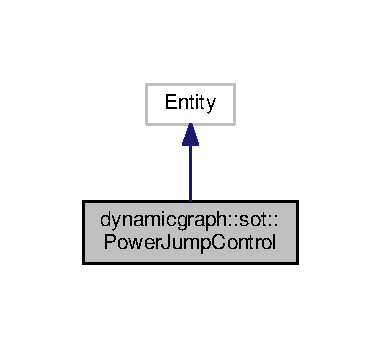
\includegraphics[width=183pt]{classdynamicgraph_1_1sot_1_1PowerJumpControl__inherit__graph}
\end{center}
\end{figure}


Collaboration diagram for dynamicgraph\+:\+:sot\+:\+:Power\+Jump\+Control\+:
\nopagebreak
\begin{figure}[H]
\begin{center}
\leavevmode
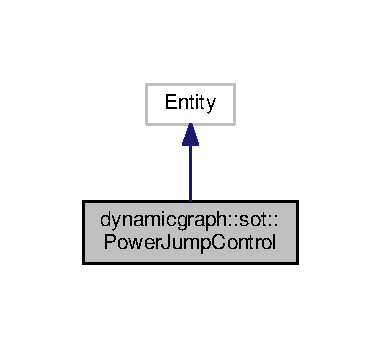
\includegraphics[width=183pt]{classdynamicgraph_1_1sot_1_1PowerJumpControl__coll__graph}
\end{center}
\end{figure}
\subsection*{Public Member Functions}
\begin{DoxyCompactItemize}
\item 
{\bfseries Power\+Jump\+Control} (const std\+::string \&name)\hypertarget{classdynamicgraph_1_1sot_1_1PowerJumpControl_aabafd0843366b3acb467e48176bc7b73}{}\label{classdynamicgraph_1_1sot_1_1PowerJumpControl_aabafd0843366b3acb467e48176bc7b73}

\item 
void {\bfseries init} (const double \&step)\hypertarget{classdynamicgraph_1_1sot_1_1PowerJumpControl_a5dd3a47fb9562e5d0092548b9fd24065}{}\label{classdynamicgraph_1_1sot_1_1PowerJumpControl_a5dd3a47fb9562e5d0092548b9fd24065}

\item 
virtual const std\+::string \& {\bfseries get\+Class\+Name} (void) const \hypertarget{classdynamicgraph_1_1sot_1_1PowerJumpControl_ac41cfcea928c9b79550b4a6ae598a6f8}{}\label{classdynamicgraph_1_1sot_1_1PowerJumpControl_ac41cfcea928c9b79550b4a6ae598a6f8}

\end{DoxyCompactItemize}
\subsection*{Public Attributes}
\begin{DoxyCompactItemize}
\item 
Signal\+Ptr$<$ dg\+::\+Vector, int $>$ {\bfseries leg\+\_\+length\+S\+IN}\hypertarget{classdynamicgraph_1_1sot_1_1PowerJumpControl_a79f096ba891251435e3ffdd9e37d7146}{}\label{classdynamicgraph_1_1sot_1_1PowerJumpControl_a79f096ba891251435e3ffdd9e37d7146}

\item 
Signal\+Ptr$<$ dg\+::\+Vector, int $>$ {\bfseries cnt\+\_\+sensor\+S\+IN}\hypertarget{classdynamicgraph_1_1sot_1_1PowerJumpControl_a8e4e534a8cfe66f3c8694d543ccf7e03}{}\label{classdynamicgraph_1_1sot_1_1PowerJumpControl_a8e4e534a8cfe66f3c8694d543ccf7e03}

\item 
Signal\+Ptr$<$ dg\+::\+Vector, int $>$ {\bfseries leg\+\_\+length\+\_\+trigger\+S\+IN}\hypertarget{classdynamicgraph_1_1sot_1_1PowerJumpControl_a5d90d4751a6d7cbac379e75f18aa552b}{}\label{classdynamicgraph_1_1sot_1_1PowerJumpControl_a5d90d4751a6d7cbac379e75f18aa552b}

\item 
Signal\+Ptr$<$ dg\+::\+Vector, int $>$ {\bfseries leg\+\_\+length\+\_\+air\+S\+IN}\hypertarget{classdynamicgraph_1_1sot_1_1PowerJumpControl_a764a3c773710d43021f7357169e26a92}{}\label{classdynamicgraph_1_1sot_1_1PowerJumpControl_a764a3c773710d43021f7357169e26a92}

\item 
Signal\+Ptr$<$ dg\+::\+Vector, int $>$ {\bfseries des\+\_\+fff\+S\+IN}\hypertarget{classdynamicgraph_1_1sot_1_1PowerJumpControl_acf3aeda51c157679d846aea4d534fd5f}{}\label{classdynamicgraph_1_1sot_1_1PowerJumpControl_acf3aeda51c157679d846aea4d534fd5f}

\item 
Signal\+Ptr$<$ dg\+::\+Vector, int $>$ {\bfseries des\+\_\+weight\+\_\+fff\+S\+IN}\hypertarget{classdynamicgraph_1_1sot_1_1PowerJumpControl_a22bbb3ec98196791f646dcdd59d2a210}{}\label{classdynamicgraph_1_1sot_1_1PowerJumpControl_a22bbb3ec98196791f646dcdd59d2a210}

\item 
Signal\+Ptr$<$ dg\+::\+Vector, int $>$ {\bfseries kp\+\_\+ground\+S\+IN}\hypertarget{classdynamicgraph_1_1sot_1_1PowerJumpControl_a05cb046fa4f52dd1f25720e633012489}{}\label{classdynamicgraph_1_1sot_1_1PowerJumpControl_a05cb046fa4f52dd1f25720e633012489}

\item 
Signal\+Ptr$<$ dg\+::\+Vector, int $>$ {\bfseries kp\+\_\+air\+S\+IN}\hypertarget{classdynamicgraph_1_1sot_1_1PowerJumpControl_af871c1aec159c961bfd93f7eb39b98f3}{}\label{classdynamicgraph_1_1sot_1_1PowerJumpControl_af871c1aec159c961bfd93f7eb39b98f3}

\item 
Signal\+Time\+Dependent$<$ dg\+::\+Vector, int $>$ {\bfseries return\+\_\+des\+\_\+pos\+S\+O\+UT}\hypertarget{classdynamicgraph_1_1sot_1_1PowerJumpControl_a5613880b3676a473dab4c970423132b0}{}\label{classdynamicgraph_1_1sot_1_1PowerJumpControl_a5613880b3676a473dab4c970423132b0}

\item 
Signal\+Time\+Dependent$<$ dg\+::\+Vector, int $>$ {\bfseries return\+\_\+des\+\_\+force\+S\+O\+UT}\hypertarget{classdynamicgraph_1_1sot_1_1PowerJumpControl_a52b5f90b8013acf3d41c9afc6849eb96}{}\label{classdynamicgraph_1_1sot_1_1PowerJumpControl_a52b5f90b8013acf3d41c9afc6849eb96}

\item 
Signal\+Time\+Dependent$<$ dg\+::\+Vector, int $>$ {\bfseries return\+\_\+des\+\_\+kp\+S\+O\+UT}\hypertarget{classdynamicgraph_1_1sot_1_1PowerJumpControl_a6403ae6d5d835ac513fbfa90de7f66a0}{}\label{classdynamicgraph_1_1sot_1_1PowerJumpControl_a6403ae6d5d835ac513fbfa90de7f66a0}

\end{DoxyCompactItemize}
\subsection*{Static Public Attributes}
\begin{DoxyCompactItemize}
\item 
static const double {\bfseries T\+I\+M\+E\+\_\+\+S\+T\+E\+P\+\_\+\+D\+E\+F\+A\+U\+LT}\hypertarget{classdynamicgraph_1_1sot_1_1PowerJumpControl_aca39789e27aa56bf6f820bbe92c89422}{}\label{classdynamicgraph_1_1sot_1_1PowerJumpControl_aca39789e27aa56bf6f820bbe92c89422}

\item 
static const std\+::string {\bfseries C\+L\+A\+S\+S\+\_\+\+N\+A\+ME}\hypertarget{classdynamicgraph_1_1sot_1_1PowerJumpControl_a4cfb045d8bedf64bf0b15801fa66c848}{}\label{classdynamicgraph_1_1sot_1_1PowerJumpControl_a4cfb045d8bedf64bf0b15801fa66c848}

\end{DoxyCompactItemize}
\subsection*{Protected Member Functions}
\begin{DoxyCompactItemize}
\item 
dg\+::\+Vector \& \hyperlink{classdynamicgraph_1_1sot_1_1PowerJumpControl_ad132ac991b6fb6cddd9aa019a33425e9}{return\+\_\+des\+\_\+pos} (dg\+::\+Vector \&des\+\_\+pos, int t)
\item 
dg\+::\+Vector \& \hyperlink{classdynamicgraph_1_1sot_1_1PowerJumpControl_a0172cfef3c8c11b441fee7380c69c227}{return\+\_\+des\+\_\+force} (dg\+::\+Vector \&des\+\_\+force, int t)
\item 
dg\+::\+Vector \& \hyperlink{classdynamicgraph_1_1sot_1_1PowerJumpControl_aa00816d8369775112bcb93b915790926}{return\+\_\+des\+\_\+kp} (dg\+::\+Vector \&des\+\_\+kp, int t)
\end{DoxyCompactItemize}
\subsection*{Protected Attributes}
\begin{DoxyCompactItemize}
\item 
double {\bfseries Time\+Step}\hypertarget{classdynamicgraph_1_1sot_1_1PowerJumpControl_a791dadb09401879a56034869b0b3b9be}{}\label{classdynamicgraph_1_1sot_1_1PowerJumpControl_a791dadb09401879a56034869b0b3b9be}

\item 
int {\bfseries pos\+\_\+trigger\+\_\+flag\+\_\+}\hypertarget{classdynamicgraph_1_1sot_1_1PowerJumpControl_aba54ff31f75ea7b32e735dde24061093}{}\label{classdynamicgraph_1_1sot_1_1PowerJumpControl_aba54ff31f75ea7b32e735dde24061093}

\item 
int {\bfseries force\+\_\+trigger\+\_\+flag\+\_\+}\hypertarget{classdynamicgraph_1_1sot_1_1PowerJumpControl_a86e8dc105cf169265bc1b183c7187e55}{}\label{classdynamicgraph_1_1sot_1_1PowerJumpControl_a86e8dc105cf169265bc1b183c7187e55}

\item 
int {\bfseries kp\+\_\+trigger\+\_\+flag\+\_\+}\hypertarget{classdynamicgraph_1_1sot_1_1PowerJumpControl_a55f86a204909e655a1f3a8deff024770}{}\label{classdynamicgraph_1_1sot_1_1PowerJumpControl_a55f86a204909e655a1f3a8deff024770}

\end{DoxyCompactItemize}


\subsection{Member Function Documentation}
\index{dynamicgraph\+::sot\+::\+Power\+Jump\+Control@{dynamicgraph\+::sot\+::\+Power\+Jump\+Control}!return\+\_\+des\+\_\+force@{return\+\_\+des\+\_\+force}}
\index{return\+\_\+des\+\_\+force@{return\+\_\+des\+\_\+force}!dynamicgraph\+::sot\+::\+Power\+Jump\+Control@{dynamicgraph\+::sot\+::\+Power\+Jump\+Control}}
\subsubsection[{\texorpdfstring{return\+\_\+des\+\_\+force(dg\+::\+Vector \&des\+\_\+force, int t)}{return_des_force(dg::Vector &des_force, int t)}}]{\setlength{\rightskip}{0pt plus 5cm}dynamicgraph\+::\+Vector \& Power\+Jump\+Control\+::return\+\_\+des\+\_\+force (
\begin{DoxyParamCaption}
\item[{dg\+::\+Vector \&}]{des\+\_\+force, }
\item[{int}]{t}
\end{DoxyParamCaption}
)\hspace{0.3cm}{\ttfamily [protected]}}\hypertarget{classdynamicgraph_1_1sot_1_1PowerJumpControl_a0172cfef3c8c11b441fee7380c69c227}{}\label{classdynamicgraph_1_1sot_1_1PowerJumpControl_a0172cfef3c8c11b441fee7380c69c227}
This method computes desired forces depending on state of the teststand \index{dynamicgraph\+::sot\+::\+Power\+Jump\+Control@{dynamicgraph\+::sot\+::\+Power\+Jump\+Control}!return\+\_\+des\+\_\+kp@{return\+\_\+des\+\_\+kp}}
\index{return\+\_\+des\+\_\+kp@{return\+\_\+des\+\_\+kp}!dynamicgraph\+::sot\+::\+Power\+Jump\+Control@{dynamicgraph\+::sot\+::\+Power\+Jump\+Control}}
\subsubsection[{\texorpdfstring{return\+\_\+des\+\_\+kp(dg\+::\+Vector \&des\+\_\+kp, int t)}{return_des_kp(dg::Vector &des_kp, int t)}}]{\setlength{\rightskip}{0pt plus 5cm}dynamicgraph\+::\+Vector \& Power\+Jump\+Control\+::return\+\_\+des\+\_\+kp (
\begin{DoxyParamCaption}
\item[{dg\+::\+Vector \&}]{des\+\_\+kp, }
\item[{int}]{t}
\end{DoxyParamCaption}
)\hspace{0.3cm}{\ttfamily [protected]}}\hypertarget{classdynamicgraph_1_1sot_1_1PowerJumpControl_aa00816d8369775112bcb93b915790926}{}\label{classdynamicgraph_1_1sot_1_1PowerJumpControl_aa00816d8369775112bcb93b915790926}
This method computes desired kp gain depending on state of the teststand \index{dynamicgraph\+::sot\+::\+Power\+Jump\+Control@{dynamicgraph\+::sot\+::\+Power\+Jump\+Control}!return\+\_\+des\+\_\+pos@{return\+\_\+des\+\_\+pos}}
\index{return\+\_\+des\+\_\+pos@{return\+\_\+des\+\_\+pos}!dynamicgraph\+::sot\+::\+Power\+Jump\+Control@{dynamicgraph\+::sot\+::\+Power\+Jump\+Control}}
\subsubsection[{\texorpdfstring{return\+\_\+des\+\_\+pos(dg\+::\+Vector \&des\+\_\+pos, int t)}{return_des_pos(dg::Vector &des_pos, int t)}}]{\setlength{\rightskip}{0pt plus 5cm}dynamicgraph\+::\+Vector \& Power\+Jump\+Control\+::return\+\_\+des\+\_\+pos (
\begin{DoxyParamCaption}
\item[{dg\+::\+Vector \&}]{des\+\_\+pos, }
\item[{int}]{t}
\end{DoxyParamCaption}
)\hspace{0.3cm}{\ttfamily [protected]}}\hypertarget{classdynamicgraph_1_1sot_1_1PowerJumpControl_ad132ac991b6fb6cddd9aa019a33425e9}{}\label{classdynamicgraph_1_1sot_1_1PowerJumpControl_ad132ac991b6fb6cddd9aa019a33425e9}
This method computes desired position depending on state of the teststand 

The documentation for this class was generated from the following files\+:\begin{DoxyCompactItemize}
\item 
include/dg\+\_\+tools/test\+\_\+stand\+\_\+control/\hyperlink{power__jump_8hpp}{power\+\_\+jump.\+hpp}\item 
src/test\+\_\+stand\+\_\+control/power\+\_\+jump.\+cpp\end{DoxyCompactItemize}

\hypertarget{classdg__tools_1_1PreviousValue}{}\section{dg\+\_\+tools\+:\+:Previous\+Value Class Reference}
\label{classdg__tools_1_1PreviousValue}\index{dg\+\_\+tools\+::\+Previous\+Value@{dg\+\_\+tools\+::\+Previous\+Value}}


Records data over a fixed history and yields the data as truncated vector.  




{\ttfamily \#include $<$previous\+\_\+value.\+hpp$>$}



Inheritance diagram for dg\+\_\+tools\+:\+:Previous\+Value\+:
\nopagebreak
\begin{figure}[H]
\begin{center}
\leavevmode
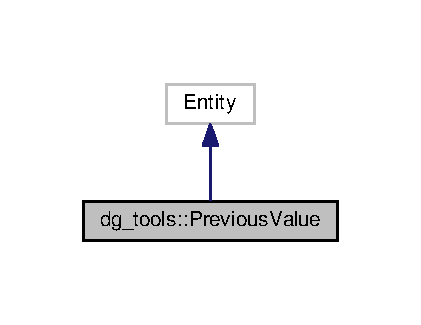
\includegraphics[width=202pt]{classdg__tools_1_1PreviousValue__inherit__graph}
\end{center}
\end{figure}


Collaboration diagram for dg\+\_\+tools\+:\+:Previous\+Value\+:
\nopagebreak
\begin{figure}[H]
\begin{center}
\leavevmode
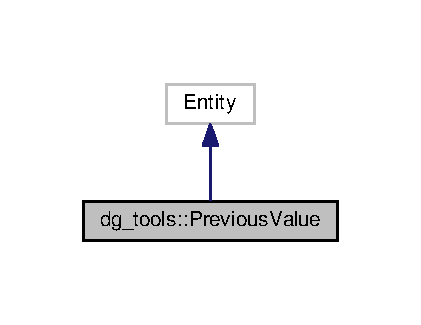
\includegraphics[width=202pt]{classdg__tools_1_1PreviousValue__coll__graph}
\end{center}
\end{figure}
\subsection*{Public Member Functions}
\begin{DoxyCompactItemize}
\item 
{\bfseries Previous\+Value} (const std\+::string \&name)\hypertarget{classdg__tools_1_1PreviousValue_a829ab1d9ddeed58307e669c3716d7adc}{}\label{classdg__tools_1_1PreviousValue_a829ab1d9ddeed58307e669c3716d7adc}

\item 
void {\bfseries init} (const int \&size)\hypertarget{classdg__tools_1_1PreviousValue_ac84ba4e47fd88946279439cc8d9a255f}{}\label{classdg__tools_1_1PreviousValue_ac84ba4e47fd88946279439cc8d9a255f}

\item 
virtual void {\bfseries display} (std\+::ostream \&os) const \hypertarget{classdg__tools_1_1PreviousValue_a5e7f1792ed7f5b43a5bb5cd6f2be9ef6}{}\label{classdg__tools_1_1PreviousValue_a5e7f1792ed7f5b43a5bb5cd6f2be9ef6}

\item 
virtual const std\+::string \& {\bfseries get\+Class\+Name} (void) const \hypertarget{classdg__tools_1_1PreviousValue_ac053765749bc6e92e81b0f0cc6d7c792}{}\label{classdg__tools_1_1PreviousValue_ac053765749bc6e92e81b0f0cc6d7c792}

\item 
dg\+::\+Vector \& {\bfseries get\+Previous} (dg\+::\+Vector \&previous, int time)\hypertarget{classdg__tools_1_1PreviousValue_a3a27aa9156c258ee6222f8212eb0d1e5}{}\label{classdg__tools_1_1PreviousValue_a3a27aa9156c258ee6222f8212eb0d1e5}

\item 
dg\+::\+Vector \& {\bfseries get\+Input} (dg\+::\+Vector \&output, int time)\hypertarget{classdg__tools_1_1PreviousValue_a034d2baec32ec23757f21a82b99e8d72}{}\label{classdg__tools_1_1PreviousValue_a034d2baec32ec23757f21a82b99e8d72}

\end{DoxyCompactItemize}
\subsection*{Public Attributes}
\begin{DoxyCompactItemize}
\item 
dg\+::\+Signal\+Ptr$<$ dg\+::\+Vector, int $>$ {\bfseries data\+S\+IN}\hypertarget{classdg__tools_1_1PreviousValue_a937b59c8319a7facb7289eff6235f0a1}{}\label{classdg__tools_1_1PreviousValue_a937b59c8319a7facb7289eff6235f0a1}

\item 
dg\+::\+Signal\+Time\+Dependent$<$ dg\+::\+Vector, int $>$ {\bfseries data\+S\+O\+UT}\hypertarget{classdg__tools_1_1PreviousValue_a655e7f859fcf867524ff51d319612b81}{}\label{classdg__tools_1_1PreviousValue_a655e7f859fcf867524ff51d319612b81}

\item 
dg\+::\+Signal\+Time\+Dependent$<$ dg\+::\+Vector, int $>$ {\bfseries previous\+S\+O\+UT}\hypertarget{classdg__tools_1_1PreviousValue_a5c76ee891d5ca88769a8b681f8c10bcc}{}\label{classdg__tools_1_1PreviousValue_a5c76ee891d5ca88769a8b681f8c10bcc}

\end{DoxyCompactItemize}
\subsection*{Static Public Attributes}
\begin{DoxyCompactItemize}
\item 
static const std\+::string {\bfseries C\+L\+A\+S\+S\+\_\+\+N\+A\+ME}\hypertarget{classdg__tools_1_1PreviousValue_ae1bcc71c1bdae70ad54f4ba7aa741a6e}{}\label{classdg__tools_1_1PreviousValue_ae1bcc71c1bdae70ad54f4ba7aa741a6e}

\end{DoxyCompactItemize}
\subsection*{Private Attributes}
\begin{DoxyCompactItemize}
\item 
int {\bfseries size\+\_\+}\hypertarget{classdg__tools_1_1PreviousValue_a343c9292b3dd5f53a02da9c1ebe70cab}{}\label{classdg__tools_1_1PreviousValue_a343c9292b3dd5f53a02da9c1ebe70cab}

\item 
bool {\bfseries is\+\_\+initialized\+\_\+}\hypertarget{classdg__tools_1_1PreviousValue_aa972a5500930267a6fd84c5570254c22}{}\label{classdg__tools_1_1PreviousValue_aa972a5500930267a6fd84c5570254c22}

\item 
dg\+::\+Vector {\bfseries internal\+\_\+history\+\_\+}\hypertarget{classdg__tools_1_1PreviousValue_aae52a34a0b2e5a8049efb66dc1b80439}{}\label{classdg__tools_1_1PreviousValue_aae52a34a0b2e5a8049efb66dc1b80439}

\end{DoxyCompactItemize}


\subsection{Detailed Description}
Records data over a fixed history and yields the data as truncated vector. 

The newest entry is at the last position of the data array,

history = \mbox{[}data\+\_\+\{t-\/n\}, data\+\_\+\{t-\/n+1\}, ..., data\+\_\+\{t-\/1\}, data\+\_\+\{t\}\mbox{]} 

The documentation for this class was generated from the following files\+:\begin{DoxyCompactItemize}
\item 
include/dg\+\_\+tools/data/previous\+\_\+value.\+hpp\item 
src/data/previous\+\_\+value.\+cpp\end{DoxyCompactItemize}

\hypertarget{classpython_1_1dg__tools_1_1leg__impedance__control_1_1quad__leg__impedance__controller_1_1QuadrupedComControl}{}\section{python.\+dg\+\_\+tools.\+leg\+\_\+impedance\+\_\+control.\+quad\+\_\+leg\+\_\+impedance\+\_\+controller.\+Quadruped\+Com\+Control Class Reference}
\label{classpython_1_1dg__tools_1_1leg__impedance__control_1_1quad__leg__impedance__controller_1_1QuadrupedComControl}\index{python.\+dg\+\_\+tools.\+leg\+\_\+impedance\+\_\+control.\+quad\+\_\+leg\+\_\+impedance\+\_\+controller.\+Quadruped\+Com\+Control@{python.\+dg\+\_\+tools.\+leg\+\_\+impedance\+\_\+control.\+quad\+\_\+leg\+\_\+impedance\+\_\+controller.\+Quadruped\+Com\+Control}}


Inheritance diagram for python.\+dg\+\_\+tools.\+leg\+\_\+impedance\+\_\+control.\+quad\+\_\+leg\+\_\+impedance\+\_\+controller.\+Quadruped\+Com\+Control\+:
\nopagebreak
\begin{figure}[H]
\begin{center}
\leavevmode
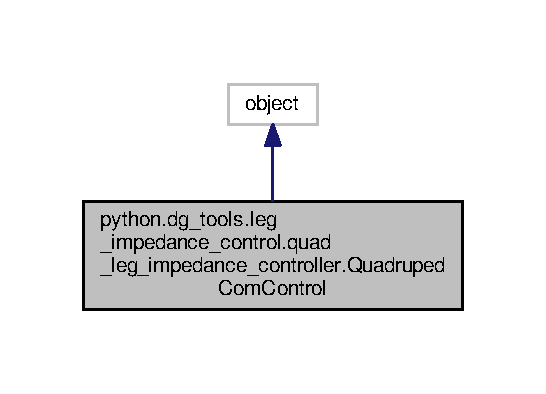
\includegraphics[width=262pt]{classpython_1_1dg__tools_1_1leg__impedance__control_1_1quad__leg__impedance__controller_1_1QuadrupedComControl__inherit__graph}
\end{center}
\end{figure}


Collaboration diagram for python.\+dg\+\_\+tools.\+leg\+\_\+impedance\+\_\+control.\+quad\+\_\+leg\+\_\+impedance\+\_\+controller.\+Quadruped\+Com\+Control\+:
\nopagebreak
\begin{figure}[H]
\begin{center}
\leavevmode
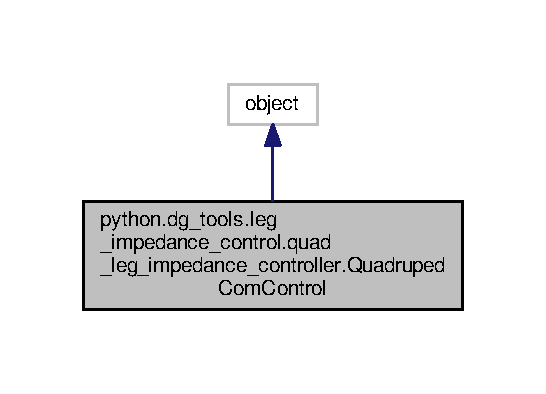
\includegraphics[width=262pt]{classpython_1_1dg__tools_1_1leg__impedance__control_1_1quad__leg__impedance__controller_1_1QuadrupedComControl__coll__graph}
\end{center}
\end{figure}
\subsection*{Public Member Functions}
\begin{DoxyCompactItemize}
\item 
def \hyperlink{classpython_1_1dg__tools_1_1leg__impedance__control_1_1quad__leg__impedance__controller_1_1QuadrupedComControl_a79f0bfd4d6bec7c6db16a92dfcbae34d}{\+\_\+\+\_\+init\+\_\+\+\_\+} (self, robot, Vicon\+Client\+Entity=None, client\+\_\+name=\char`\"{}vicon\+\_\+client\char`\"{}, vicon\+\_\+ip=\textquotesingle{}10.\+32.\+3.\+16\+:801\textquotesingle{}, Entity\+Name=\char`\"{}quad\+\_\+com\+\_\+ctrl\char`\"{}, base\+\_\+position=None, base\+\_\+velocity=None)
\item 
def {\bfseries init\+\_\+robot\+\_\+properties} (self)\hypertarget{classpython_1_1dg__tools_1_1leg__impedance__control_1_1quad__leg__impedance__controller_1_1QuadrupedComControl_a24959d27c6da979857fa30013833441b}{}\label{classpython_1_1dg__tools_1_1leg__impedance__control_1_1quad__leg__impedance__controller_1_1QuadrupedComControl_a24959d27c6da979857fa30013833441b}

\item 
def {\bfseries compute\+\_\+torques} (self, Kp, des\+\_\+pos, Kd, des\+\_\+vel, des\+\_\+fff)\hypertarget{classpython_1_1dg__tools_1_1leg__impedance__control_1_1quad__leg__impedance__controller_1_1QuadrupedComControl_a7d000c801d5acd59cc68d91e58b3b1d3}{}\label{classpython_1_1dg__tools_1_1leg__impedance__control_1_1quad__leg__impedance__controller_1_1QuadrupedComControl_a7d000c801d5acd59cc68d91e58b3b1d3}

\item 
def \hyperlink{classpython_1_1dg__tools_1_1leg__impedance__control_1_1quad__leg__impedance__controller_1_1QuadrupedComControl_abb466e86a2c54b0c3d0aebe6142dbc4b}{compute\+\_\+ang\+\_\+control\+\_\+torques} (self, Kp\+\_\+ang, des\+\_\+ori, Kd\+\_\+ang, des\+\_\+ang\+\_\+vel, des\+\_\+fft)\hypertarget{classpython_1_1dg__tools_1_1leg__impedance__control_1_1quad__leg__impedance__controller_1_1QuadrupedComControl_abb466e86a2c54b0c3d0aebe6142dbc4b}{}\label{classpython_1_1dg__tools_1_1leg__impedance__control_1_1quad__leg__impedance__controller_1_1QuadrupedComControl_abb466e86a2c54b0c3d0aebe6142dbc4b}

\begin{DoxyCompactList}\small\item\em \paragraph*{Computes torques required to control the orientation of base}\end{DoxyCompactList}\item 
def {\bfseries set\+\_\+bias} (self)\hypertarget{classpython_1_1dg__tools_1_1leg__impedance__control_1_1quad__leg__impedance__controller_1_1QuadrupedComControl_aeba77303f6d204751b7b2d376fa44531}{}\label{classpython_1_1dg__tools_1_1leg__impedance__control_1_1quad__leg__impedance__controller_1_1QuadrupedComControl_aeba77303f6d204751b7b2d376fa44531}

\item 
def \hyperlink{classpython_1_1dg__tools_1_1leg__impedance__control_1_1quad__leg__impedance__controller_1_1QuadrupedComControl_a471495c1adac63c6cb9a521fea0b52d6}{get\+\_\+biased\+\_\+base\+\_\+position} (self)
\begin{DoxyCompactList}\small\item\em Return the robot position taking the bias offset into account. \end{DoxyCompactList}\item 
def \hyperlink{classpython_1_1dg__tools_1_1leg__impedance__control_1_1quad__leg__impedance__controller_1_1QuadrupedComControl_af130be175b4257723b48248e1ec41ab4}{get\+\_\+biased\+\_\+base\+\_\+velocity} (self)
\begin{DoxyCompactList}\small\item\em Return the robot velocity taking the bias offset into account. \end{DoxyCompactList}\item 
def {\bfseries set\+\_\+abs\+\_\+end\+\_\+eff\+\_\+pos} (self, abs\+\_\+end\+\_\+eff\+\_\+pos\+\_\+sig)\hypertarget{classpython_1_1dg__tools_1_1leg__impedance__control_1_1quad__leg__impedance__controller_1_1QuadrupedComControl_a722398d4df248546c7316ef3e4cf35ec}{}\label{classpython_1_1dg__tools_1_1leg__impedance__control_1_1quad__leg__impedance__controller_1_1QuadrupedComControl_a722398d4df248546c7316ef3e4cf35ec}

\item 
def {\bfseries threshold\+\_\+cnt\+\_\+sensor} (self)\hypertarget{classpython_1_1dg__tools_1_1leg__impedance__control_1_1quad__leg__impedance__controller_1_1QuadrupedComControl_a9c37016b0e903660cbf38885b9bee52e}{}\label{classpython_1_1dg__tools_1_1leg__impedance__control_1_1quad__leg__impedance__controller_1_1QuadrupedComControl_a9c37016b0e903660cbf38885b9bee52e}

\item 
def {\bfseries convert\+\_\+cnt\+\_\+value\+\_\+to\+\_\+3d} (self, cnt\+\_\+sensor, start\+\_\+index, end\+\_\+index, entity\+Name)\hypertarget{classpython_1_1dg__tools_1_1leg__impedance__control_1_1quad__leg__impedance__controller_1_1QuadrupedComControl_aebd187dc86fdc93f43c8991c14af8c52}{}\label{classpython_1_1dg__tools_1_1leg__impedance__control_1_1quad__leg__impedance__controller_1_1QuadrupedComControl_aebd187dc86fdc93f43c8991c14af8c52}

\item 
def \hyperlink{classpython_1_1dg__tools_1_1leg__impedance__control_1_1quad__leg__impedance__controller_1_1QuadrupedComControl_a7b2d46aa0abd8e9ced9e3cce2147d124}{return\+\_\+lqr\+\_\+tau} (self, des\+\_\+pos, des\+\_\+vel, des\+\_\+ori, des\+\_\+ang\+\_\+vel, des\+\_\+fff, des\+\_\+fft, des\+\_\+lqr)
\begin{DoxyCompactList}\small\item\em \paragraph*{for lqr based controller.}\end{DoxyCompactList}\item 
def \hyperlink{classpython_1_1dg__tools_1_1leg__impedance__control_1_1quad__leg__impedance__controller_1_1QuadrupedComControl_a68a8b7ea897a69259d9409e0f703b7d3}{return\+\_\+end\+\_\+eff\+\_\+lqr\+\_\+tau} (self, des\+\_\+pos, des\+\_\+vel, des\+\_\+ori, des\+\_\+ang\+\_\+vel, des\+\_\+fff, des\+\_\+lqr)
\begin{DoxyCompactList}\small\item\em \paragraph*{for lqr based controller at the end effector.}\end{DoxyCompactList}\item 
def {\bfseries return\+\_\+com\+\_\+torques} (self, com\+\_\+tau, ang\+\_\+tau, des\+\_\+abs\+\_\+vel, hess, g0, ce, ci, ci0, reg, cnt\+\_\+plan=None)\hypertarget{classpython_1_1dg__tools_1_1leg__impedance__control_1_1quad__leg__impedance__controller_1_1QuadrupedComControl_a44644610db1d8cce8f1bbe31c4225382}{}\label{classpython_1_1dg__tools_1_1leg__impedance__control_1_1quad__leg__impedance__controller_1_1QuadrupedComControl_a44644610db1d8cce8f1bbe31c4225382}

\item 
def {\bfseries record\+\_\+data} (self)\hypertarget{classpython_1_1dg__tools_1_1leg__impedance__control_1_1quad__leg__impedance__controller_1_1QuadrupedComControl_a40cbf1bb320c3c8272346a988b190051}{}\label{classpython_1_1dg__tools_1_1leg__impedance__control_1_1quad__leg__impedance__controller_1_1QuadrupedComControl_a40cbf1bb320c3c8272346a988b190051}

\end{DoxyCompactItemize}
\subsection*{Public Attributes}
\begin{DoxyCompactItemize}
\item 
{\bfseries robot}\hypertarget{classpython_1_1dg__tools_1_1leg__impedance__control_1_1quad__leg__impedance__controller_1_1QuadrupedComControl_a488eecc9d4462202d8bb53602927db9c}{}\label{classpython_1_1dg__tools_1_1leg__impedance__control_1_1quad__leg__impedance__controller_1_1QuadrupedComControl_a488eecc9d4462202d8bb53602927db9c}

\item 
{\bfseries Entity\+Name}\hypertarget{classpython_1_1dg__tools_1_1leg__impedance__control_1_1quad__leg__impedance__controller_1_1QuadrupedComControl_a82f0b7c3180f2f9715dd92708581a8de}{}\label{classpython_1_1dg__tools_1_1leg__impedance__control_1_1quad__leg__impedance__controller_1_1QuadrupedComControl_a82f0b7c3180f2f9715dd92708581a8de}

\item 
{\bfseries client\+\_\+name}\hypertarget{classpython_1_1dg__tools_1_1leg__impedance__control_1_1quad__leg__impedance__controller_1_1QuadrupedComControl_a13da8028b3e77cf5a4d2fdaef725bffe}{}\label{classpython_1_1dg__tools_1_1leg__impedance__control_1_1quad__leg__impedance__controller_1_1QuadrupedComControl_a13da8028b3e77cf5a4d2fdaef725bffe}

\item 
{\bfseries host\+\_\+name\+\_\+quadruped}\hypertarget{classpython_1_1dg__tools_1_1leg__impedance__control_1_1quad__leg__impedance__controller_1_1QuadrupedComControl_ade7b6029cb3100520e1aa478b4277019}{}\label{classpython_1_1dg__tools_1_1leg__impedance__control_1_1quad__leg__impedance__controller_1_1QuadrupedComControl_ade7b6029cb3100520e1aa478b4277019}

\item 
{\bfseries vicon\+\_\+client}\hypertarget{classpython_1_1dg__tools_1_1leg__impedance__control_1_1quad__leg__impedance__controller_1_1QuadrupedComControl_a98858d4caa17f4359c5acdea327c7ee3}{}\label{classpython_1_1dg__tools_1_1leg__impedance__control_1_1quad__leg__impedance__controller_1_1QuadrupedComControl_a98858d4caa17f4359c5acdea327c7ee3}

\item 
\hyperlink{classpython_1_1dg__tools_1_1leg__impedance__control_1_1quad__leg__impedance__controller_1_1QuadrupedComControl_a695c53b1d3f3048db84a33a2d028d2d2}{vicon\+\_\+base\+\_\+position}\hypertarget{classpython_1_1dg__tools_1_1leg__impedance__control_1_1quad__leg__impedance__controller_1_1QuadrupedComControl_a695c53b1d3f3048db84a33a2d028d2d2}{}\label{classpython_1_1dg__tools_1_1leg__impedance__control_1_1quad__leg__impedance__controller_1_1QuadrupedComControl_a695c53b1d3f3048db84a33a2d028d2d2}

\begin{DoxyCompactList}\small\item\em comment out if running on real robot \end{DoxyCompactList}\item 
{\bfseries vicon\+\_\+base\+\_\+velocity}\hypertarget{classpython_1_1dg__tools_1_1leg__impedance__control_1_1quad__leg__impedance__controller_1_1QuadrupedComControl_a1c6239d0a6491040ef0b7d71acc5e1e8}{}\label{classpython_1_1dg__tools_1_1leg__impedance__control_1_1quad__leg__impedance__controller_1_1QuadrupedComControl_a1c6239d0a6491040ef0b7d71acc5e1e8}

\item 
{\bfseries com\+\_\+imp\+\_\+ctrl}\hypertarget{classpython_1_1dg__tools_1_1leg__impedance__control_1_1quad__leg__impedance__controller_1_1QuadrupedComControl_a28ca164b0b8abfdd0f451a8953a737e9}{}\label{classpython_1_1dg__tools_1_1leg__impedance__control_1_1quad__leg__impedance__controller_1_1QuadrupedComControl_a28ca164b0b8abfdd0f451a8953a737e9}

\item 
{\bfseries vicon\+\_\+offset}\hypertarget{classpython_1_1dg__tools_1_1leg__impedance__control_1_1quad__leg__impedance__controller_1_1QuadrupedComControl_a6f4dfb8c993ea388b065b9eb6abcef03}{}\label{classpython_1_1dg__tools_1_1leg__impedance__control_1_1quad__leg__impedance__controller_1_1QuadrupedComControl_a6f4dfb8c993ea388b065b9eb6abcef03}

\item 
{\bfseries robot\+\_\+vicon\+\_\+name}\hypertarget{classpython_1_1dg__tools_1_1leg__impedance__control_1_1quad__leg__impedance__controller_1_1QuadrupedComControl_a4f07757912f99abaea2a60467583caff}{}\label{classpython_1_1dg__tools_1_1leg__impedance__control_1_1quad__leg__impedance__controller_1_1QuadrupedComControl_a4f07757912f99abaea2a60467583caff}

\item 
{\bfseries robot\+\_\+mass}\hypertarget{classpython_1_1dg__tools_1_1leg__impedance__control_1_1quad__leg__impedance__controller_1_1QuadrupedComControl_a87d507ec32ac2a6901ae04b827376569}{}\label{classpython_1_1dg__tools_1_1leg__impedance__control_1_1quad__leg__impedance__controller_1_1QuadrupedComControl_a87d507ec32ac2a6901ae04b827376569}

\item 
{\bfseries robot\+\_\+base\+\_\+inertia}\hypertarget{classpython_1_1dg__tools_1_1leg__impedance__control_1_1quad__leg__impedance__controller_1_1QuadrupedComControl_a3786caaa2be0b24a5347adeca6bb952f}{}\label{classpython_1_1dg__tools_1_1leg__impedance__control_1_1quad__leg__impedance__controller_1_1QuadrupedComControl_a3786caaa2be0b24a5347adeca6bb952f}

\item 
{\bfseries base\+\_\+pos\+\_\+xyz}\hypertarget{classpython_1_1dg__tools_1_1leg__impedance__control_1_1quad__leg__impedance__controller_1_1QuadrupedComControl_aac090bcc93ca706025c8b57d8f8e0042}{}\label{classpython_1_1dg__tools_1_1leg__impedance__control_1_1quad__leg__impedance__controller_1_1QuadrupedComControl_aac090bcc93ca706025c8b57d8f8e0042}

\item 
{\bfseries base\+\_\+vel\+\_\+xyz}\hypertarget{classpython_1_1dg__tools_1_1leg__impedance__control_1_1quad__leg__impedance__controller_1_1QuadrupedComControl_abd3dafeed32eb38408f8fd0e9977b923}{}\label{classpython_1_1dg__tools_1_1leg__impedance__control_1_1quad__leg__impedance__controller_1_1QuadrupedComControl_abd3dafeed32eb38408f8fd0e9977b923}

\item 
\hyperlink{classpython_1_1dg__tools_1_1leg__impedance__control_1_1quad__leg__impedance__controller_1_1QuadrupedComControl_a8e10de9b174c7e0d0a4e02c90697ca32}{control\+\_\+switch\+\_\+pos}\hypertarget{classpython_1_1dg__tools_1_1leg__impedance__control_1_1quad__leg__impedance__controller_1_1QuadrupedComControl_a8e10de9b174c7e0d0a4e02c90697ca32}{}\label{classpython_1_1dg__tools_1_1leg__impedance__control_1_1quad__leg__impedance__controller_1_1QuadrupedComControl_a8e10de9b174c7e0d0a4e02c90697ca32}

\begin{DoxyCompactList}\small\item\em mass in all direction (double to vec returns zero) T\+O\+DO \+: Check if there is dynamicgraph\+::double \end{DoxyCompactList}\item 
{\bfseries control\+\_\+switch\+\_\+vel}\hypertarget{classpython_1_1dg__tools_1_1leg__impedance__control_1_1quad__leg__impedance__controller_1_1QuadrupedComControl_a78d353fbc468b24675b1c49fe9c12c2e}{}\label{classpython_1_1dg__tools_1_1leg__impedance__control_1_1quad__leg__impedance__controller_1_1QuadrupedComControl_a78d353fbc468b24675b1c49fe9c12c2e}

\item 
{\bfseries biased\+\_\+base\+\_\+pos\+\_\+xyz}\hypertarget{classpython_1_1dg__tools_1_1leg__impedance__control_1_1quad__leg__impedance__controller_1_1QuadrupedComControl_a3e8ac246a42a33475e381d2a1e1f338d}{}\label{classpython_1_1dg__tools_1_1leg__impedance__control_1_1quad__leg__impedance__controller_1_1QuadrupedComControl_a3e8ac246a42a33475e381d2a1e1f338d}

\item 
{\bfseries biased\+\_\+base\+\_\+vel\+\_\+xyz}\hypertarget{classpython_1_1dg__tools_1_1leg__impedance__control_1_1quad__leg__impedance__controller_1_1QuadrupedComControl_a0dc4bd5452d58aea5234d5a190a4d4c7}{}\label{classpython_1_1dg__tools_1_1leg__impedance__control_1_1quad__leg__impedance__controller_1_1QuadrupedComControl_a0dc4bd5452d58aea5234d5a190a4d4c7}

\item 
{\bfseries torques}\hypertarget{classpython_1_1dg__tools_1_1leg__impedance__control_1_1quad__leg__impedance__controller_1_1QuadrupedComControl_a105e881a685bbb0e83a2a19d3fbd8e6f}{}\label{classpython_1_1dg__tools_1_1leg__impedance__control_1_1quad__leg__impedance__controller_1_1QuadrupedComControl_a105e881a685bbb0e83a2a19d3fbd8e6f}

\item 
{\bfseries base\+\_\+orientation}\hypertarget{classpython_1_1dg__tools_1_1leg__impedance__control_1_1quad__leg__impedance__controller_1_1QuadrupedComControl_a6c1e1b68c68c6531b920c79ce5a42806}{}\label{classpython_1_1dg__tools_1_1leg__impedance__control_1_1quad__leg__impedance__controller_1_1QuadrupedComControl_a6c1e1b68c68c6531b920c79ce5a42806}

\item 
{\bfseries base\+\_\+ang\+\_\+vel\+\_\+xyz}\hypertarget{classpython_1_1dg__tools_1_1leg__impedance__control_1_1quad__leg__impedance__controller_1_1QuadrupedComControl_a6b8a3f691df20c4ea6020c2dc6e30d82}{}\label{classpython_1_1dg__tools_1_1leg__impedance__control_1_1quad__leg__impedance__controller_1_1QuadrupedComControl_a6b8a3f691df20c4ea6020c2dc6e30d82}

\item 
\hyperlink{classpython_1_1dg__tools_1_1leg__impedance__control_1_1quad__leg__impedance__controller_1_1QuadrupedComControl_a91ffd9fe58d946e2326b05b5f808c8f4}{wb\+\_\+ctrl}\hypertarget{classpython_1_1dg__tools_1_1leg__impedance__control_1_1quad__leg__impedance__controller_1_1QuadrupedComControl_a91ffd9fe58d946e2326b05b5f808c8f4}{}\label{classpython_1_1dg__tools_1_1leg__impedance__control_1_1quad__leg__impedance__controller_1_1QuadrupedComControl_a91ffd9fe58d946e2326b05b5f808c8f4}

\begin{DoxyCompactList}\small\item\em This divides forces using the wbc controller. \end{DoxyCompactList}\end{DoxyCompactItemize}
\subsection*{Private Attributes}
\begin{DoxyCompactItemize}
\item 
{\bfseries \+\_\+biased\+\_\+base\+\_\+position}\hypertarget{classpython_1_1dg__tools_1_1leg__impedance__control_1_1quad__leg__impedance__controller_1_1QuadrupedComControl_af39670c39353751a4b619aaa750db486}{}\label{classpython_1_1dg__tools_1_1leg__impedance__control_1_1quad__leg__impedance__controller_1_1QuadrupedComControl_af39670c39353751a4b619aaa750db486}

\item 
{\bfseries \+\_\+biased\+\_\+base\+\_\+velocity}\hypertarget{classpython_1_1dg__tools_1_1leg__impedance__control_1_1quad__leg__impedance__controller_1_1QuadrupedComControl_a45789c40361ce8f788984be0ee845c97}{}\label{classpython_1_1dg__tools_1_1leg__impedance__control_1_1quad__leg__impedance__controller_1_1QuadrupedComControl_a45789c40361ce8f788984be0ee845c97}

\end{DoxyCompactItemize}


\subsection{Constructor \& Destructor Documentation}
\index{python\+::dg\+\_\+tools\+::leg\+\_\+impedance\+\_\+control\+::quad\+\_\+leg\+\_\+impedance\+\_\+controller\+::\+Quadruped\+Com\+Control@{python\+::dg\+\_\+tools\+::leg\+\_\+impedance\+\_\+control\+::quad\+\_\+leg\+\_\+impedance\+\_\+controller\+::\+Quadruped\+Com\+Control}!\+\_\+\+\_\+init\+\_\+\+\_\+@{\+\_\+\+\_\+init\+\_\+\+\_\+}}
\index{\+\_\+\+\_\+init\+\_\+\+\_\+@{\+\_\+\+\_\+init\+\_\+\+\_\+}!python\+::dg\+\_\+tools\+::leg\+\_\+impedance\+\_\+control\+::quad\+\_\+leg\+\_\+impedance\+\_\+controller\+::\+Quadruped\+Com\+Control@{python\+::dg\+\_\+tools\+::leg\+\_\+impedance\+\_\+control\+::quad\+\_\+leg\+\_\+impedance\+\_\+controller\+::\+Quadruped\+Com\+Control}}
\subsubsection[{\texorpdfstring{\+\_\+\+\_\+init\+\_\+\+\_\+(self, robot, Vicon\+Client\+Entity=\+None, client\+\_\+name=""vicon\+\_\+client"", vicon\+\_\+ip=\textquotesingle{}10.\+32.\+3.\+16\+:801\textquotesingle{}, Entity\+Name=""quad\+\_\+com\+\_\+ctrl"", base\+\_\+position=\+None, base\+\_\+velocity=\+None)}{__init__(self, robot, ViconClientEntity=None, client_name="vicon_client", vicon_ip='10.32.3.16:801', EntityName="quad_com_ctrl", base_position=None, base_velocity=None)}}]{\setlength{\rightskip}{0pt plus 5cm}def python.\+dg\+\_\+tools.\+leg\+\_\+impedance\+\_\+control.\+quad\+\_\+leg\+\_\+impedance\+\_\+controller.\+Quadruped\+Com\+Control.\+\_\+\+\_\+init\+\_\+\+\_\+ (
\begin{DoxyParamCaption}
\item[{}]{self, }
\item[{}]{robot, }
\item[{}]{Vicon\+Client\+Entity = {\ttfamily None}, }
\item[{}]{client\+\_\+name = {\ttfamily \char`\"{}vicon\+\_\+client\char`\"{}}, }
\item[{}]{vicon\+\_\+ip = {\ttfamily \textquotesingle{}10.32.3.16\+:801\textquotesingle{}}, }
\item[{}]{Entity\+Name = {\ttfamily \char`\"{}quad\+\_\+com\+\_\+ctrl\char`\"{}}, }
\item[{}]{base\+\_\+position = {\ttfamily None}, }
\item[{}]{base\+\_\+velocity = {\ttfamily None}}
\end{DoxyParamCaption}
)}\hypertarget{classpython_1_1dg__tools_1_1leg__impedance__control_1_1quad__leg__impedance__controller_1_1QuadrupedComControl_a79f0bfd4d6bec7c6db16a92dfcbae34d}{}\label{classpython_1_1dg__tools_1_1leg__impedance__control_1_1quad__leg__impedance__controller_1_1QuadrupedComControl_a79f0bfd4d6bec7c6db16a92dfcbae34d}

\begin{DoxyParams}{Parameters}
{\em base\+\_\+position} & (Optional, Vec7d signal) Base position of the robot. \\
\hline
{\em base\+\_\+velocity} & (Optional, Vec6d signal) Base velocity of the robot. \\
\hline
\end{DoxyParams}


\subsection{Member Function Documentation}
\index{python\+::dg\+\_\+tools\+::leg\+\_\+impedance\+\_\+control\+::quad\+\_\+leg\+\_\+impedance\+\_\+controller\+::\+Quadruped\+Com\+Control@{python\+::dg\+\_\+tools\+::leg\+\_\+impedance\+\_\+control\+::quad\+\_\+leg\+\_\+impedance\+\_\+controller\+::\+Quadruped\+Com\+Control}!get\+\_\+biased\+\_\+base\+\_\+position@{get\+\_\+biased\+\_\+base\+\_\+position}}
\index{get\+\_\+biased\+\_\+base\+\_\+position@{get\+\_\+biased\+\_\+base\+\_\+position}!python\+::dg\+\_\+tools\+::leg\+\_\+impedance\+\_\+control\+::quad\+\_\+leg\+\_\+impedance\+\_\+controller\+::\+Quadruped\+Com\+Control@{python\+::dg\+\_\+tools\+::leg\+\_\+impedance\+\_\+control\+::quad\+\_\+leg\+\_\+impedance\+\_\+controller\+::\+Quadruped\+Com\+Control}}
\subsubsection[{\texorpdfstring{get\+\_\+biased\+\_\+base\+\_\+position(self)}{get_biased_base_position(self)}}]{\setlength{\rightskip}{0pt plus 5cm}def python.\+dg\+\_\+tools.\+leg\+\_\+impedance\+\_\+control.\+quad\+\_\+leg\+\_\+impedance\+\_\+controller.\+Quadruped\+Com\+Control.\+get\+\_\+biased\+\_\+base\+\_\+position (
\begin{DoxyParamCaption}
\item[{}]{self}
\end{DoxyParamCaption}
)}\hypertarget{classpython_1_1dg__tools_1_1leg__impedance__control_1_1quad__leg__impedance__controller_1_1QuadrupedComControl_a471495c1adac63c6cb9a521fea0b52d6}{}\label{classpython_1_1dg__tools_1_1leg__impedance__control_1_1quad__leg__impedance__controller_1_1QuadrupedComControl_a471495c1adac63c6cb9a521fea0b52d6}


Return the robot position taking the bias offset into account. 

\begin{DoxyReturn}{Returns}
Signal$<$dg\+::vector$>$ of size 7 (0\+:3 translation, 3\+:7 quaternion orientation) 
\end{DoxyReturn}
\index{python\+::dg\+\_\+tools\+::leg\+\_\+impedance\+\_\+control\+::quad\+\_\+leg\+\_\+impedance\+\_\+controller\+::\+Quadruped\+Com\+Control@{python\+::dg\+\_\+tools\+::leg\+\_\+impedance\+\_\+control\+::quad\+\_\+leg\+\_\+impedance\+\_\+controller\+::\+Quadruped\+Com\+Control}!get\+\_\+biased\+\_\+base\+\_\+velocity@{get\+\_\+biased\+\_\+base\+\_\+velocity}}
\index{get\+\_\+biased\+\_\+base\+\_\+velocity@{get\+\_\+biased\+\_\+base\+\_\+velocity}!python\+::dg\+\_\+tools\+::leg\+\_\+impedance\+\_\+control\+::quad\+\_\+leg\+\_\+impedance\+\_\+controller\+::\+Quadruped\+Com\+Control@{python\+::dg\+\_\+tools\+::leg\+\_\+impedance\+\_\+control\+::quad\+\_\+leg\+\_\+impedance\+\_\+controller\+::\+Quadruped\+Com\+Control}}
\subsubsection[{\texorpdfstring{get\+\_\+biased\+\_\+base\+\_\+velocity(self)}{get_biased_base_velocity(self)}}]{\setlength{\rightskip}{0pt plus 5cm}def python.\+dg\+\_\+tools.\+leg\+\_\+impedance\+\_\+control.\+quad\+\_\+leg\+\_\+impedance\+\_\+controller.\+Quadruped\+Com\+Control.\+get\+\_\+biased\+\_\+base\+\_\+velocity (
\begin{DoxyParamCaption}
\item[{}]{self}
\end{DoxyParamCaption}
)}\hypertarget{classpython_1_1dg__tools_1_1leg__impedance__control_1_1quad__leg__impedance__controller_1_1QuadrupedComControl_af130be175b4257723b48248e1ec41ab4}{}\label{classpython_1_1dg__tools_1_1leg__impedance__control_1_1quad__leg__impedance__controller_1_1QuadrupedComControl_af130be175b4257723b48248e1ec41ab4}


Return the robot velocity taking the bias offset into account. 

\begin{DoxyReturn}{Returns}
Signal$<$dg\+::vector$>$ of size 6 (0\+:3 translation, 3\+:6 rpy orientation) 
\end{DoxyReturn}
\index{python\+::dg\+\_\+tools\+::leg\+\_\+impedance\+\_\+control\+::quad\+\_\+leg\+\_\+impedance\+\_\+controller\+::\+Quadruped\+Com\+Control@{python\+::dg\+\_\+tools\+::leg\+\_\+impedance\+\_\+control\+::quad\+\_\+leg\+\_\+impedance\+\_\+controller\+::\+Quadruped\+Com\+Control}!return\+\_\+end\+\_\+eff\+\_\+lqr\+\_\+tau@{return\+\_\+end\+\_\+eff\+\_\+lqr\+\_\+tau}}
\index{return\+\_\+end\+\_\+eff\+\_\+lqr\+\_\+tau@{return\+\_\+end\+\_\+eff\+\_\+lqr\+\_\+tau}!python\+::dg\+\_\+tools\+::leg\+\_\+impedance\+\_\+control\+::quad\+\_\+leg\+\_\+impedance\+\_\+controller\+::\+Quadruped\+Com\+Control@{python\+::dg\+\_\+tools\+::leg\+\_\+impedance\+\_\+control\+::quad\+\_\+leg\+\_\+impedance\+\_\+controller\+::\+Quadruped\+Com\+Control}}
\subsubsection[{\texorpdfstring{return\+\_\+end\+\_\+eff\+\_\+lqr\+\_\+tau(self, des\+\_\+pos, des\+\_\+vel, des\+\_\+ori, des\+\_\+ang\+\_\+vel, des\+\_\+fff, des\+\_\+lqr)}{return_end_eff_lqr_tau(self, des_pos, des_vel, des_ori, des_ang_vel, des_fff, des_lqr)}}]{\setlength{\rightskip}{0pt plus 5cm}def python.\+dg\+\_\+tools.\+leg\+\_\+impedance\+\_\+control.\+quad\+\_\+leg\+\_\+impedance\+\_\+controller.\+Quadruped\+Com\+Control.\+return\+\_\+end\+\_\+eff\+\_\+lqr\+\_\+tau (
\begin{DoxyParamCaption}
\item[{}]{self, }
\item[{}]{des\+\_\+pos, }
\item[{}]{des\+\_\+vel, }
\item[{}]{des\+\_\+ori, }
\item[{}]{des\+\_\+ang\+\_\+vel, }
\item[{}]{des\+\_\+fff, }
\item[{}]{des\+\_\+lqr}
\end{DoxyParamCaption}
)}\hypertarget{classpython_1_1dg__tools_1_1leg__impedance__control_1_1quad__leg__impedance__controller_1_1QuadrupedComControl_a68a8b7ea897a69259d9409e0f703b7d3}{}\label{classpython_1_1dg__tools_1_1leg__impedance__control_1_1quad__leg__impedance__controller_1_1QuadrupedComControl_a68a8b7ea897a69259d9409e0f703b7d3}


\paragraph*{for lqr based controller at the end effector.}

reads values obtained from the planner \index{python\+::dg\+\_\+tools\+::leg\+\_\+impedance\+\_\+control\+::quad\+\_\+leg\+\_\+impedance\+\_\+controller\+::\+Quadruped\+Com\+Control@{python\+::dg\+\_\+tools\+::leg\+\_\+impedance\+\_\+control\+::quad\+\_\+leg\+\_\+impedance\+\_\+controller\+::\+Quadruped\+Com\+Control}!return\+\_\+lqr\+\_\+tau@{return\+\_\+lqr\+\_\+tau}}
\index{return\+\_\+lqr\+\_\+tau@{return\+\_\+lqr\+\_\+tau}!python\+::dg\+\_\+tools\+::leg\+\_\+impedance\+\_\+control\+::quad\+\_\+leg\+\_\+impedance\+\_\+controller\+::\+Quadruped\+Com\+Control@{python\+::dg\+\_\+tools\+::leg\+\_\+impedance\+\_\+control\+::quad\+\_\+leg\+\_\+impedance\+\_\+controller\+::\+Quadruped\+Com\+Control}}
\subsubsection[{\texorpdfstring{return\+\_\+lqr\+\_\+tau(self, des\+\_\+pos, des\+\_\+vel, des\+\_\+ori, des\+\_\+ang\+\_\+vel, des\+\_\+fff, des\+\_\+fft, des\+\_\+lqr)}{return_lqr_tau(self, des_pos, des_vel, des_ori, des_ang_vel, des_fff, des_fft, des_lqr)}}]{\setlength{\rightskip}{0pt plus 5cm}def python.\+dg\+\_\+tools.\+leg\+\_\+impedance\+\_\+control.\+quad\+\_\+leg\+\_\+impedance\+\_\+controller.\+Quadruped\+Com\+Control.\+return\+\_\+lqr\+\_\+tau (
\begin{DoxyParamCaption}
\item[{}]{self, }
\item[{}]{des\+\_\+pos, }
\item[{}]{des\+\_\+vel, }
\item[{}]{des\+\_\+ori, }
\item[{}]{des\+\_\+ang\+\_\+vel, }
\item[{}]{des\+\_\+fff, }
\item[{}]{des\+\_\+fft, }
\item[{}]{des\+\_\+lqr}
\end{DoxyParamCaption}
)}\hypertarget{classpython_1_1dg__tools_1_1leg__impedance__control_1_1quad__leg__impedance__controller_1_1QuadrupedComControl_a7b2d46aa0abd8e9ced9e3cce2147d124}{}\label{classpython_1_1dg__tools_1_1leg__impedance__control_1_1quad__leg__impedance__controller_1_1QuadrupedComControl_a7b2d46aa0abd8e9ced9e3cce2147d124}


\paragraph*{for lqr based controller.}

reads values obtained from the planner 

The documentation for this class was generated from the following file\+:\begin{DoxyCompactItemize}
\item 
python/dg\+\_\+tools/leg\+\_\+impedance\+\_\+control/\hyperlink{quad__leg__impedance__controller_8py}{quad\+\_\+leg\+\_\+impedance\+\_\+controller.\+py}\end{DoxyCompactItemize}

\hypertarget{classpython_1_1dg__tools_1_1leg__impedance__control_1_1quad__leg__impedance__controller_1_1QuadrupedLegImpedanceController}{}\section{python.\+dg\+\_\+tools.\+leg\+\_\+impedance\+\_\+control.\+quad\+\_\+leg\+\_\+impedance\+\_\+controller.\+Quadruped\+Leg\+Impedance\+Controller Class Reference}
\label{classpython_1_1dg__tools_1_1leg__impedance__control_1_1quad__leg__impedance__controller_1_1QuadrupedLegImpedanceController}\index{python.\+dg\+\_\+tools.\+leg\+\_\+impedance\+\_\+control.\+quad\+\_\+leg\+\_\+impedance\+\_\+controller.\+Quadruped\+Leg\+Impedance\+Controller@{python.\+dg\+\_\+tools.\+leg\+\_\+impedance\+\_\+control.\+quad\+\_\+leg\+\_\+impedance\+\_\+controller.\+Quadruped\+Leg\+Impedance\+Controller}}
\subsection*{Public Member Functions}
\begin{DoxyCompactItemize}
\item 
def {\bfseries \+\_\+\+\_\+init\+\_\+\+\_\+} (self, robot)\hypertarget{classpython_1_1dg__tools_1_1leg__impedance__control_1_1quad__leg__impedance__controller_1_1QuadrupedLegImpedanceController_afc8023b76557c43c7c78728e2c488a13}{}\label{classpython_1_1dg__tools_1_1leg__impedance__control_1_1quad__leg__impedance__controller_1_1QuadrupedLegImpedanceController_afc8023b76557c43c7c78728e2c488a13}

\item 
def {\bfseries return\+\_\+control\+\_\+torques} (self, kp, des\+\_\+pos, kd=None, des\+\_\+vel=None, kf=None, fff=None)\hypertarget{classpython_1_1dg__tools_1_1leg__impedance__control_1_1quad__leg__impedance__controller_1_1QuadrupedLegImpedanceController_ac088ea885c8fd492b7530ab324a6c13d}{}\label{classpython_1_1dg__tools_1_1leg__impedance__control_1_1quad__leg__impedance__controller_1_1QuadrupedLegImpedanceController_ac088ea885c8fd492b7530ab324a6c13d}

\item 
def {\bfseries return\+\_\+joint\+\_\+ctrl\+\_\+torques} (self, kp\+\_\+joint, des\+\_\+joint\+\_\+pos, kd\+\_\+joint, des\+\_\+joint\+\_\+vel)\hypertarget{classpython_1_1dg__tools_1_1leg__impedance__control_1_1quad__leg__impedance__controller_1_1QuadrupedLegImpedanceController_a3771f36bdc425fe25f9ea7be910be6cc}{}\label{classpython_1_1dg__tools_1_1leg__impedance__control_1_1quad__leg__impedance__controller_1_1QuadrupedLegImpedanceController_a3771f36bdc425fe25f9ea7be910be6cc}

\item 
def {\bfseries record\+\_\+data} (self, record\+\_\+vicon=False)\hypertarget{classpython_1_1dg__tools_1_1leg__impedance__control_1_1quad__leg__impedance__controller_1_1QuadrupedLegImpedanceController_a4255058eb1cde0133b86e4833ce76eb8}{}\label{classpython_1_1dg__tools_1_1leg__impedance__control_1_1quad__leg__impedance__controller_1_1QuadrupedLegImpedanceController_a4255058eb1cde0133b86e4833ce76eb8}

\end{DoxyCompactItemize}
\subsection*{Public Attributes}
\begin{DoxyCompactItemize}
\item 
{\bfseries robot}\hypertarget{classpython_1_1dg__tools_1_1leg__impedance__control_1_1quad__leg__impedance__controller_1_1QuadrupedLegImpedanceController_ac27f3b4ad26d2fc0c23d73efaa3bffdb}{}\label{classpython_1_1dg__tools_1_1leg__impedance__control_1_1quad__leg__impedance__controller_1_1QuadrupedLegImpedanceController_ac27f3b4ad26d2fc0c23d73efaa3bffdb}

\item 
{\bfseries imp\+\_\+ctrl\+\_\+leg\+\_\+fl}\hypertarget{classpython_1_1dg__tools_1_1leg__impedance__control_1_1quad__leg__impedance__controller_1_1QuadrupedLegImpedanceController_a099a3736c547979bb639de5def48a7d5}{}\label{classpython_1_1dg__tools_1_1leg__impedance__control_1_1quad__leg__impedance__controller_1_1QuadrupedLegImpedanceController_a099a3736c547979bb639de5def48a7d5}

\item 
{\bfseries imp\+\_\+ctrl\+\_\+leg\+\_\+fr}\hypertarget{classpython_1_1dg__tools_1_1leg__impedance__control_1_1quad__leg__impedance__controller_1_1QuadrupedLegImpedanceController_a5fb205521b76d5a25dda5c1a3a912501}{}\label{classpython_1_1dg__tools_1_1leg__impedance__control_1_1quad__leg__impedance__controller_1_1QuadrupedLegImpedanceController_a5fb205521b76d5a25dda5c1a3a912501}

\item 
{\bfseries imp\+\_\+ctrl\+\_\+leg\+\_\+hl}\hypertarget{classpython_1_1dg__tools_1_1leg__impedance__control_1_1quad__leg__impedance__controller_1_1QuadrupedLegImpedanceController_a533c02f2d6ac458d6526712b153efdfd}{}\label{classpython_1_1dg__tools_1_1leg__impedance__control_1_1quad__leg__impedance__controller_1_1QuadrupedLegImpedanceController_a533c02f2d6ac458d6526712b153efdfd}

\item 
{\bfseries imp\+\_\+ctrl\+\_\+leg\+\_\+hr}\hypertarget{classpython_1_1dg__tools_1_1leg__impedance__control_1_1quad__leg__impedance__controller_1_1QuadrupedLegImpedanceController_ad21bde4b52a2a2474b7fdb1b5f2b5cf1}{}\label{classpython_1_1dg__tools_1_1leg__impedance__control_1_1quad__leg__impedance__controller_1_1QuadrupedLegImpedanceController_ad21bde4b52a2a2474b7fdb1b5f2b5cf1}

\item 
{\bfseries joint\+\_\+positions}\hypertarget{classpython_1_1dg__tools_1_1leg__impedance__control_1_1quad__leg__impedance__controller_1_1QuadrupedLegImpedanceController_a0530f8803b7f7b59fe3d7a8dfcee45d8}{}\label{classpython_1_1dg__tools_1_1leg__impedance__control_1_1quad__leg__impedance__controller_1_1QuadrupedLegImpedanceController_a0530f8803b7f7b59fe3d7a8dfcee45d8}

\item 
{\bfseries joint\+\_\+velocities}\hypertarget{classpython_1_1dg__tools_1_1leg__impedance__control_1_1quad__leg__impedance__controller_1_1QuadrupedLegImpedanceController_a6ffc1716a029c75c48c144650a4795fa}{}\label{classpython_1_1dg__tools_1_1leg__impedance__control_1_1quad__leg__impedance__controller_1_1QuadrupedLegImpedanceController_a6ffc1716a029c75c48c144650a4795fa}

\end{DoxyCompactItemize}


The documentation for this class was generated from the following file\+:\begin{DoxyCompactItemize}
\item 
python/dg\+\_\+tools/leg\+\_\+impedance\+\_\+control/\hyperlink{quad__leg__impedance__controller_8py}{quad\+\_\+leg\+\_\+impedance\+\_\+controller.\+py}\end{DoxyCompactItemize}

\hypertarget{classdynamicgraph_1_1sot_1_1ReactiveLQRController}{}\section{dynamicgraph\+:\+:sot\+:\+:Reactive\+L\+Q\+R\+Controller Class Reference}
\label{classdynamicgraph_1_1sot_1_1ReactiveLQRController}\index{dynamicgraph\+::sot\+::\+Reactive\+L\+Q\+R\+Controller@{dynamicgraph\+::sot\+::\+Reactive\+L\+Q\+R\+Controller}}


Inheritance diagram for dynamicgraph\+:\+:sot\+:\+:Reactive\+L\+Q\+R\+Controller\+:
\nopagebreak
\begin{figure}[H]
\begin{center}
\leavevmode
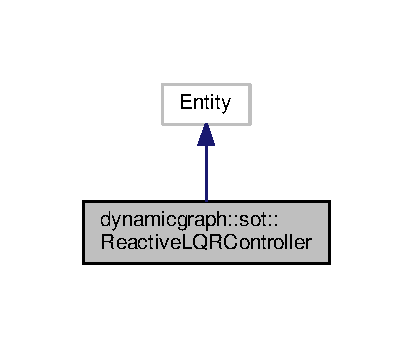
\includegraphics[width=198pt]{classdynamicgraph_1_1sot_1_1ReactiveLQRController__inherit__graph}
\end{center}
\end{figure}


Collaboration diagram for dynamicgraph\+:\+:sot\+:\+:Reactive\+L\+Q\+R\+Controller\+:
\nopagebreak
\begin{figure}[H]
\begin{center}
\leavevmode
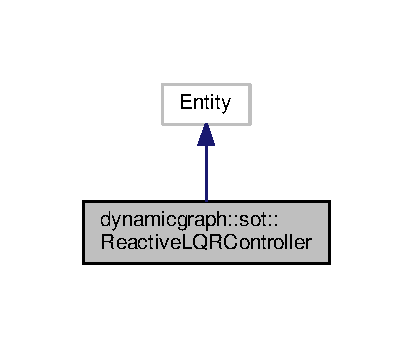
\includegraphics[width=198pt]{classdynamicgraph_1_1sot_1_1ReactiveLQRController__coll__graph}
\end{center}
\end{figure}
\subsection*{Public Member Functions}
\begin{DoxyCompactItemize}
\item 
{\bfseries Reactive\+L\+Q\+R\+Controller} (const std\+::string \&name)\hypertarget{classdynamicgraph_1_1sot_1_1ReactiveLQRController_adadf8983289573506586a2816bafd341}{}\label{classdynamicgraph_1_1sot_1_1ReactiveLQRController_adadf8983289573506586a2816bafd341}

\item 
void {\bfseries init} (const double \&step)\hypertarget{classdynamicgraph_1_1sot_1_1ReactiveLQRController_a451edaa3e541b7cebd4cb35c60df3d5f}{}\label{classdynamicgraph_1_1sot_1_1ReactiveLQRController_a451edaa3e541b7cebd4cb35c60df3d5f}

\item 
virtual const std\+::string \& {\bfseries get\+Class\+Name} (void) const \hypertarget{classdynamicgraph_1_1sot_1_1ReactiveLQRController_a9ce5a32886f5a7ed3690a1a1e04c64f1}{}\label{classdynamicgraph_1_1sot_1_1ReactiveLQRController_a9ce5a32886f5a7ed3690a1a1e04c64f1}

\end{DoxyCompactItemize}
\subsection*{Public Attributes}
\begin{DoxyCompactItemize}
\item 
Signal\+Ptr$<$ dg\+::\+Vector, int $>$ {\bfseries com\+\_\+pos\+S\+IN}\hypertarget{classdynamicgraph_1_1sot_1_1ReactiveLQRController_a9f050fe73c1207aed8e4e2476058a5d7}{}\label{classdynamicgraph_1_1sot_1_1ReactiveLQRController_a9f050fe73c1207aed8e4e2476058a5d7}

\item 
Signal\+Ptr$<$ dg\+::\+Vector, int $>$ {\bfseries com\+\_\+vel\+S\+IN}\hypertarget{classdynamicgraph_1_1sot_1_1ReactiveLQRController_a37ed7a82a1de99a7345cf214e54788a6}{}\label{classdynamicgraph_1_1sot_1_1ReactiveLQRController_a37ed7a82a1de99a7345cf214e54788a6}

\item 
Signal\+Ptr$<$ dg\+::\+Vector, int $>$ {\bfseries com\+\_\+ori\+S\+IN}\hypertarget{classdynamicgraph_1_1sot_1_1ReactiveLQRController_a4239a94f19bea395df844325bc8affe7}{}\label{classdynamicgraph_1_1sot_1_1ReactiveLQRController_a4239a94f19bea395df844325bc8affe7}

\item 
Signal\+Ptr$<$ dg\+::\+Vector, int $>$ {\bfseries com\+\_\+ang\+\_\+vel\+S\+IN}\hypertarget{classdynamicgraph_1_1sot_1_1ReactiveLQRController_afb4e2cac8e956735d947c5ec52563d95}{}\label{classdynamicgraph_1_1sot_1_1ReactiveLQRController_afb4e2cac8e956735d947c5ec52563d95}

\item 
Signal\+Ptr$<$ dg\+::\+Vector, int $>$ {\bfseries end\+\_\+eff\+\_\+pos\+\_\+12d\+S\+IN}\hypertarget{classdynamicgraph_1_1sot_1_1ReactiveLQRController_aad5fe0754c7b6d6384b6acf823f38903}{}\label{classdynamicgraph_1_1sot_1_1ReactiveLQRController_aad5fe0754c7b6d6384b6acf823f38903}

\item 
Signal\+Ptr$<$ dg\+::\+Vector, int $>$ {\bfseries des\+\_\+fff\+S\+IN}\hypertarget{classdynamicgraph_1_1sot_1_1ReactiveLQRController_a67aae768a9f98cb7540db11bbff81f2d}{}\label{classdynamicgraph_1_1sot_1_1ReactiveLQRController_a67aae768a9f98cb7540db11bbff81f2d}

\item 
Signal\+Ptr$<$ dg\+::\+Vector, int $>$ {\bfseries cnt\+\_\+value\+S\+IN}\hypertarget{classdynamicgraph_1_1sot_1_1ReactiveLQRController_a12b49987af52f764eecaeb788ecd48a3}{}\label{classdynamicgraph_1_1sot_1_1ReactiveLQRController_a12b49987af52f764eecaeb788ecd48a3}

\item 
Signal\+Ptr$<$ dg\+::\+Vector, int $>$ {\bfseries cnt\+\_\+sensor\+\_\+value\+S\+IN}\hypertarget{classdynamicgraph_1_1sot_1_1ReactiveLQRController_a3781cc897a995d70e2e80e040cde8c3d}{}\label{classdynamicgraph_1_1sot_1_1ReactiveLQRController_a3781cc897a995d70e2e80e040cde8c3d}

\item 
Signal\+Ptr$<$ dg\+::\+Vector, int $>$ {\bfseries state\+\_\+vector\+S\+IN}\hypertarget{classdynamicgraph_1_1sot_1_1ReactiveLQRController_afe8266615929ddf98edd1cbb9a112a2e}{}\label{classdynamicgraph_1_1sot_1_1ReactiveLQRController_afe8266615929ddf98edd1cbb9a112a2e}

\item 
Signal\+Ptr$<$ dg\+::\+Vector, int $>$ {\bfseries mass\+S\+IN}\hypertarget{classdynamicgraph_1_1sot_1_1ReactiveLQRController_a43817bd45fec9e9a8eac9a6c0825a0e4}{}\label{classdynamicgraph_1_1sot_1_1ReactiveLQRController_a43817bd45fec9e9a8eac9a6c0825a0e4}

\item 
Signal\+Ptr$<$ dg\+::\+Matrix, int $>$ {\bfseries inertia\+S\+IN}\hypertarget{classdynamicgraph_1_1sot_1_1ReactiveLQRController_a5e4f0fcf9c3189710dde3122ad6e2cec}{}\label{classdynamicgraph_1_1sot_1_1ReactiveLQRController_a5e4f0fcf9c3189710dde3122ad6e2cec}

\item 
Signal\+Ptr$<$ dg\+::\+Vector, int $>$ {\bfseries horizon\+S\+IN}\hypertarget{classdynamicgraph_1_1sot_1_1ReactiveLQRController_ae6ca32f6e84c49432d3f7093a3bcceed}{}\label{classdynamicgraph_1_1sot_1_1ReactiveLQRController_ae6ca32f6e84c49432d3f7093a3bcceed}

\item 
Signal\+Ptr$<$ dg\+::\+Matrix, int $>$ {\bfseries q\+S\+IN}\hypertarget{classdynamicgraph_1_1sot_1_1ReactiveLQRController_ae7d742ea626780b183b8b0659aef8e0a}{}\label{classdynamicgraph_1_1sot_1_1ReactiveLQRController_ae7d742ea626780b183b8b0659aef8e0a}

\item 
Signal\+Ptr$<$ dg\+::\+Matrix, int $>$ {\bfseries r\+S\+IN}\hypertarget{classdynamicgraph_1_1sot_1_1ReactiveLQRController_ac5a82514b41a223927707386d7cdb94b}{}\label{classdynamicgraph_1_1sot_1_1ReactiveLQRController_ac5a82514b41a223927707386d7cdb94b}

\item 
Signal\+Time\+Dependent$<$ dg\+::\+Matrix, int $>$ {\bfseries lqr\+\_\+gains\+S\+O\+UT}\hypertarget{classdynamicgraph_1_1sot_1_1ReactiveLQRController_afb4b89af55824026abc87a0a857d4565}{}\label{classdynamicgraph_1_1sot_1_1ReactiveLQRController_afb4b89af55824026abc87a0a857d4565}

\end{DoxyCompactItemize}
\subsection*{Static Public Attributes}
\begin{DoxyCompactItemize}
\item 
static const double {\bfseries T\+I\+M\+E\+\_\+\+S\+T\+E\+P\+\_\+\+D\+E\+F\+A\+U\+LT}\hypertarget{classdynamicgraph_1_1sot_1_1ReactiveLQRController_acb1e94e6054ddcf31529ec6decd6331a}{}\label{classdynamicgraph_1_1sot_1_1ReactiveLQRController_acb1e94e6054ddcf31529ec6decd6331a}

\item 
static const std\+::string {\bfseries C\+L\+A\+S\+S\+\_\+\+N\+A\+ME}\hypertarget{classdynamicgraph_1_1sot_1_1ReactiveLQRController_a53faaaa218d7358f3285bd564253f55d}{}\label{classdynamicgraph_1_1sot_1_1ReactiveLQRController_a53faaaa218d7358f3285bd564253f55d}

\end{DoxyCompactItemize}
\subsection*{Protected Member Functions}
\begin{DoxyCompactItemize}
\item 
double \& {\bfseries setsize} (int dimension)\hypertarget{classdynamicgraph_1_1sot_1_1ReactiveLQRController_ab1b84af1283057d2877292b7dc80ca10}{}\label{classdynamicgraph_1_1sot_1_1ReactiveLQRController_ab1b84af1283057d2877292b7dc80ca10}

\item 
Eigen\+::\+Vector\+Xd {\bfseries compute\+\_\+dyn\+\_\+} (Eigen\+::\+Vector3d com\+\_\+pos, Eigen\+::\+Vector3d com\+\_\+vel, Eigen\+::\+Quaternion$<$ double $>$ ori, Eigen\+::\+Vector3d com\+\_\+ang\+\_\+vel, Eigen\+::\+Vector\+Xd end\+\_\+eff\+\_\+pos\+\_\+12d, Eigen\+::\+Vector\+Xd des\+\_\+fff, Eigen\+::\+Vector4d cnt\+\_\+value, double mass, Eigen\+::\+Matrix\+Xd inertia, Eigen\+::\+Matrix\+Xd \&A\+\_\+t, Eigen\+::\+Matrix\+Xd \&B\+\_\+t)\hypertarget{classdynamicgraph_1_1sot_1_1ReactiveLQRController_a3853bde8dab7bbf2c78b8583f991c7d3}{}\label{classdynamicgraph_1_1sot_1_1ReactiveLQRController_a3853bde8dab7bbf2c78b8583f991c7d3}

\item 
void {\bfseries compute\+\_\+lin\+\_\+dyn\+\_\+} (Eigen\+::\+Matrix\+Xd lin\+\_\+\+A\+\_\+t, Eigen\+::\+Matrix\+Xd lin\+\_\+\+B\+\_\+t)\hypertarget{classdynamicgraph_1_1sot_1_1ReactiveLQRController_abe026a8e8e754a0677e6c2a3690f5e7e}{}\label{classdynamicgraph_1_1sot_1_1ReactiveLQRController_abe026a8e8e754a0677e6c2a3690f5e7e}

\item 
void {\bfseries compute\+\_\+num\+\_\+lin\+\_\+dyn\+\_\+} (Eigen\+::\+Vector3d com\+\_\+pos\+\_\+t, Eigen\+::\+Vector\+Xd com\+\_\+vel, Eigen\+::\+Vector3d com\+\_\+ang\+\_\+vel\+\_\+t, Eigen\+::\+Quaternion$<$ double $>$ ori\+\_\+t, Eigen\+::\+Vector\+Xd end\+\_\+eff\+\_\+pos\+\_\+12d\+\_\+t, Eigen\+::\+Vector4d cnt\+\_\+value\+\_\+t, Eigen\+::\+Vector3d com\+\_\+pos\+\_\+t1, Eigen\+::\+Vector3d com\+\_\+vel\+\_\+t1, Eigen\+::\+Vector3d com\+\_\+ang\+\_\+vel\+\_\+t1, Eigen\+::\+Quaternion$<$ double $>$ ori\+\_\+t1, Eigen\+::\+Vector\+Xd end\+\_\+eff\+\_\+pos\+\_\+12d\+\_\+t1, Eigen\+::\+Vector4d cnt\+\_\+value\+\_\+t1, Eigen\+::\+Vector\+Xd des\+\_\+fff, double mass, Eigen\+::\+Matrix\+Xd inertia, Eigen\+::\+Matrix\+Xd \&lin\+\_\+\+A\+\_\+t, Eigen\+::\+Matrix\+Xd \&lin\+\_\+\+B\+\_\+t)\hypertarget{classdynamicgraph_1_1sot_1_1ReactiveLQRController_a647da9f56f0891d286837b011bdc2bf2}{}\label{classdynamicgraph_1_1sot_1_1ReactiveLQRController_a647da9f56f0891d286837b011bdc2bf2}

\item 
Eigen\+::\+Matrix\+Xd {\bfseries compute\+\_\+r\+\_\+cross\+\_\+mat\+\_\+} (Eigen\+::\+Vector\+Xd end\+\_\+eff\+\_\+pos, Eigen\+::\+Vector3d com\+\_\+pos)\hypertarget{classdynamicgraph_1_1sot_1_1ReactiveLQRController_ad916eab348bd474acd0f6878930afccc}{}\label{classdynamicgraph_1_1sot_1_1ReactiveLQRController_ad916eab348bd474acd0f6878930afccc}

\item 
void {\bfseries compute\+\_\+lqr\+\_\+gains\+\_\+} (Eigen\+::\+Matrix\+Xd Q, Eigen\+::\+Matrix\+Xd R, Eigen\+::\+Matrix\+Xd lin\+\_\+A, Eigen\+::\+Matrix\+Xd lin\+\_\+B, Eigen\+::\+Matrix\+Xd P\+\_\+prev, Eigen\+::\+Matrix\+Xd \&P, Eigen\+::\+Matrix\+Xd \&K)\hypertarget{classdynamicgraph_1_1sot_1_1ReactiveLQRController_a83a4b8fe1fa38fcef3e4a8050b4c38dc}{}\label{classdynamicgraph_1_1sot_1_1ReactiveLQRController_a83a4b8fe1fa38fcef3e4a8050b4c38dc}

\item 
dynamicgraph\+::\+Matrix \& {\bfseries return\+\_\+lqr\+\_\+gains\+\_\+} (dynamicgraph\+::\+Matrix \&lqr\+\_\+gains, int t)\hypertarget{classdynamicgraph_1_1sot_1_1ReactiveLQRController_a69da0343d71b0f3a6b2695b9233158cb}{}\label{classdynamicgraph_1_1sot_1_1ReactiveLQRController_a69da0343d71b0f3a6b2695b9233158cb}

\end{DoxyCompactItemize}
\subsection*{Protected Attributes}
\begin{DoxyCompactItemize}
\item 
double {\bfseries Time\+Step}\hypertarget{classdynamicgraph_1_1sot_1_1ReactiveLQRController_a0f2586edd6a237c9de8261c181621fe2}{}\label{classdynamicgraph_1_1sot_1_1ReactiveLQRController_a0f2586edd6a237c9de8261c181621fe2}

\item 
Eigen\+::\+Matrix\+Xd {\bfseries omega}\hypertarget{classdynamicgraph_1_1sot_1_1ReactiveLQRController_a327283b07625ac76dfe84648e4e0f16a}{}\label{classdynamicgraph_1_1sot_1_1ReactiveLQRController_a327283b07625ac76dfe84648e4e0f16a}

\item 
Eigen\+::\+Matrix\+Xd {\bfseries inertia\+\_\+global\+\_\+inv}\hypertarget{classdynamicgraph_1_1sot_1_1ReactiveLQRController_a17ba2cebca46cff932bbdbd081e5c589}{}\label{classdynamicgraph_1_1sot_1_1ReactiveLQRController_a17ba2cebca46cff932bbdbd081e5c589}

\item 
Eigen\+::\+Matrix\+Xd {\bfseries mass\+\_\+inv\+\_\+identity}\hypertarget{classdynamicgraph_1_1sot_1_1ReactiveLQRController_ad88ca491bd15614cfa11420080428231}{}\label{classdynamicgraph_1_1sot_1_1ReactiveLQRController_ad88ca491bd15614cfa11420080428231}

\item 
Eigen\+::\+Matrix\+Xd {\bfseries R\+\_\+cross\+\_\+mat}\hypertarget{classdynamicgraph_1_1sot_1_1ReactiveLQRController_a2fcc55b58c71781314cf36277b413b8a}{}\label{classdynamicgraph_1_1sot_1_1ReactiveLQRController_a2fcc55b58c71781314cf36277b413b8a}

\item 
Eigen\+::\+Matrix\+Xd {\bfseries R\+\_\+cross\+\_\+mat\+\_\+fl}\hypertarget{classdynamicgraph_1_1sot_1_1ReactiveLQRController_af5995d569208fab4aba796479e953809}{}\label{classdynamicgraph_1_1sot_1_1ReactiveLQRController_af5995d569208fab4aba796479e953809}

\item 
Eigen\+::\+Matrix\+Xd {\bfseries R\+\_\+cross\+\_\+mat\+\_\+fr}\hypertarget{classdynamicgraph_1_1sot_1_1ReactiveLQRController_abc1dc457ac829f470d77fb46bac1b9f4}{}\label{classdynamicgraph_1_1sot_1_1ReactiveLQRController_abc1dc457ac829f470d77fb46bac1b9f4}

\item 
Eigen\+::\+Matrix\+Xd {\bfseries R\+\_\+cross\+\_\+mat\+\_\+hl}\hypertarget{classdynamicgraph_1_1sot_1_1ReactiveLQRController_ab2f911ed59f7718041b2ed13db4ab5c4}{}\label{classdynamicgraph_1_1sot_1_1ReactiveLQRController_ab2f911ed59f7718041b2ed13db4ab5c4}

\item 
Eigen\+::\+Matrix\+Xd {\bfseries R\+\_\+cross\+\_\+mat\+\_\+hr}\hypertarget{classdynamicgraph_1_1sot_1_1ReactiveLQRController_a5b5300e92ef8daf9c3101207e9cd43cc}{}\label{classdynamicgraph_1_1sot_1_1ReactiveLQRController_a5b5300e92ef8daf9c3101207e9cd43cc}

\item 
Eigen\+::\+Matrix\+Xd {\bfseries A\+\_\+t}\hypertarget{classdynamicgraph_1_1sot_1_1ReactiveLQRController_aef27a2c8ddb70627d585cb29ba99247a}{}\label{classdynamicgraph_1_1sot_1_1ReactiveLQRController_aef27a2c8ddb70627d585cb29ba99247a}

\item 
Eigen\+::\+Matrix\+Xd {\bfseries B\+\_\+t}\hypertarget{classdynamicgraph_1_1sot_1_1ReactiveLQRController_a52fa47d91f03030533dbe35454963643}{}\label{classdynamicgraph_1_1sot_1_1ReactiveLQRController_a52fa47d91f03030533dbe35454963643}

\item 
Eigen\+::\+Matrix\+Xd {\bfseries A\+\_\+t1}\hypertarget{classdynamicgraph_1_1sot_1_1ReactiveLQRController_a588745fec5a6a5dda7db8fa535f14608}{}\label{classdynamicgraph_1_1sot_1_1ReactiveLQRController_a588745fec5a6a5dda7db8fa535f14608}

\item 
Eigen\+::\+Matrix\+Xd {\bfseries B\+\_\+t1}\hypertarget{classdynamicgraph_1_1sot_1_1ReactiveLQRController_a0e691a6093118d79c5b9adaa872de63a}{}\label{classdynamicgraph_1_1sot_1_1ReactiveLQRController_a0e691a6093118d79c5b9adaa872de63a}

\item 
Eigen\+::\+Vector\+Xd {\bfseries x}\hypertarget{classdynamicgraph_1_1sot_1_1ReactiveLQRController_a3f97a8deea2dbc164aa1447ae7f80142}{}\label{classdynamicgraph_1_1sot_1_1ReactiveLQRController_a3f97a8deea2dbc164aa1447ae7f80142}

\item 
Eigen\+::\+Vector\+Xd {\bfseries unit\+\_\+vec}\hypertarget{classdynamicgraph_1_1sot_1_1ReactiveLQRController_a3c3c8b62b218489410c6d184aa997ae5}{}\label{classdynamicgraph_1_1sot_1_1ReactiveLQRController_a3c3c8b62b218489410c6d184aa997ae5}

\item 
Eigen\+::\+Vector3d {\bfseries com\+\_\+pos\+\_\+pd}\hypertarget{classdynamicgraph_1_1sot_1_1ReactiveLQRController_afe0998656ec3cb08389a553a9e85347d}{}\label{classdynamicgraph_1_1sot_1_1ReactiveLQRController_afe0998656ec3cb08389a553a9e85347d}

\item 
Eigen\+::\+Vector3d {\bfseries com\+\_\+vel\+\_\+pd}\hypertarget{classdynamicgraph_1_1sot_1_1ReactiveLQRController_ab0d1ff267844a6db789c018fd2dd0328}{}\label{classdynamicgraph_1_1sot_1_1ReactiveLQRController_ab0d1ff267844a6db789c018fd2dd0328}

\item 
Eigen\+::\+Vector3d {\bfseries com\+\_\+ang\+\_\+vel\+\_\+pd}\hypertarget{classdynamicgraph_1_1sot_1_1ReactiveLQRController_ac2b019f6c36a2f6ab5fe6f9ce8b179d3}{}\label{classdynamicgraph_1_1sot_1_1ReactiveLQRController_ac2b019f6c36a2f6ab5fe6f9ce8b179d3}

\item 
Eigen\+::\+Quaternion$<$ double $>$ {\bfseries com\+\_\+ori\+\_\+pd}\hypertarget{classdynamicgraph_1_1sot_1_1ReactiveLQRController_a9f0884e024d5b94a1f7d2908e0cd039e}{}\label{classdynamicgraph_1_1sot_1_1ReactiveLQRController_a9f0884e024d5b94a1f7d2908e0cd039e}

\item 
Eigen\+::\+Matrix\+Xd {\bfseries P\+\_\+prev}\hypertarget{classdynamicgraph_1_1sot_1_1ReactiveLQRController_a2541c4fd8464ff8882a442f859c1834d}{}\label{classdynamicgraph_1_1sot_1_1ReactiveLQRController_a2541c4fd8464ff8882a442f859c1834d}

\item 
Eigen\+::\+Matrix\+Xd {\bfseries K\+\_\+prev}\hypertarget{classdynamicgraph_1_1sot_1_1ReactiveLQRController_ad738da301e2fc81e08e074c0b4719917}{}\label{classdynamicgraph_1_1sot_1_1ReactiveLQRController_ad738da301e2fc81e08e074c0b4719917}

\item 
Eigen\+::\+Matrix\+Xd {\bfseries P}\hypertarget{classdynamicgraph_1_1sot_1_1ReactiveLQRController_aa64b907a780db180d4b1ccce730fdc18}{}\label{classdynamicgraph_1_1sot_1_1ReactiveLQRController_aa64b907a780db180d4b1ccce730fdc18}

\item 
Eigen\+::\+Matrix\+Xd {\bfseries K}\hypertarget{classdynamicgraph_1_1sot_1_1ReactiveLQRController_a72cd1cf49c4390ea10c6d6abae401cdc}{}\label{classdynamicgraph_1_1sot_1_1ReactiveLQRController_a72cd1cf49c4390ea10c6d6abae401cdc}

\item 
Eigen\+::\+Vector\+Xd {\bfseries com\+\_\+pos\+\_\+t}\hypertarget{classdynamicgraph_1_1sot_1_1ReactiveLQRController_ad37d6574833f4b41529d89f926d1dc69}{}\label{classdynamicgraph_1_1sot_1_1ReactiveLQRController_ad37d6574833f4b41529d89f926d1dc69}

\item 
Eigen\+::\+Vector\+Xd {\bfseries com\+\_\+vel\+\_\+t}\hypertarget{classdynamicgraph_1_1sot_1_1ReactiveLQRController_a44a588d654155a003897e2d9be705efa}{}\label{classdynamicgraph_1_1sot_1_1ReactiveLQRController_a44a588d654155a003897e2d9be705efa}

\item 
Eigen\+::\+Vector\+Xd {\bfseries com\+\_\+ang\+\_\+vel\+\_\+t}\hypertarget{classdynamicgraph_1_1sot_1_1ReactiveLQRController_af67408a608180df5e4aca8b5dc6c9e1f}{}\label{classdynamicgraph_1_1sot_1_1ReactiveLQRController_af67408a608180df5e4aca8b5dc6c9e1f}

\item 
Eigen\+::\+Vector\+Xd {\bfseries ori\+\_\+tmp}\hypertarget{classdynamicgraph_1_1sot_1_1ReactiveLQRController_ae04dc7c01af351daee615bf3fd5657da}{}\label{classdynamicgraph_1_1sot_1_1ReactiveLQRController_ae04dc7c01af351daee615bf3fd5657da}

\item 
Eigen\+::\+Quaternion$<$ double $>$ {\bfseries com\+\_\+ori\+\_\+t}\hypertarget{classdynamicgraph_1_1sot_1_1ReactiveLQRController_ab0021a695dff69e6aa4ed2c9c555ff72}{}\label{classdynamicgraph_1_1sot_1_1ReactiveLQRController_ab0021a695dff69e6aa4ed2c9c555ff72}

\item 
Eigen\+::\+Vector\+Xd {\bfseries des\+\_\+fff\+\_\+t}\hypertarget{classdynamicgraph_1_1sot_1_1ReactiveLQRController_a114a27f29f465e926074e3652c9de03a}{}\label{classdynamicgraph_1_1sot_1_1ReactiveLQRController_a114a27f29f465e926074e3652c9de03a}

\item 
Eigen\+::\+Vector\+Xd {\bfseries cnt\+\_\+value\+\_\+t}\hypertarget{classdynamicgraph_1_1sot_1_1ReactiveLQRController_a5d9cf72e492cfcfca2bbb60acb31a3a2}{}\label{classdynamicgraph_1_1sot_1_1ReactiveLQRController_a5d9cf72e492cfcfca2bbb60acb31a3a2}

\item 
Eigen\+::\+Vector\+Xd {\bfseries end\+\_\+eff\+\_\+pos\+\_\+12d\+\_\+t}\hypertarget{classdynamicgraph_1_1sot_1_1ReactiveLQRController_a1b5b9e2a1e7c095c3d7f3e9269e55f51}{}\label{classdynamicgraph_1_1sot_1_1ReactiveLQRController_a1b5b9e2a1e7c095c3d7f3e9269e55f51}

\item 
Eigen\+::\+Vector\+Xd {\bfseries xd\+\_\+t}\hypertarget{classdynamicgraph_1_1sot_1_1ReactiveLQRController_a6b443e106a886a084b0b1b39d601ec25}{}\label{classdynamicgraph_1_1sot_1_1ReactiveLQRController_a6b443e106a886a084b0b1b39d601ec25}

\item 
Eigen\+::\+Vector\+Xd {\bfseries com\+\_\+pos\+\_\+t1}\hypertarget{classdynamicgraph_1_1sot_1_1ReactiveLQRController_a5c4d3a7cbb4ef11b6b59a9244bc56b4f}{}\label{classdynamicgraph_1_1sot_1_1ReactiveLQRController_a5c4d3a7cbb4ef11b6b59a9244bc56b4f}

\item 
Eigen\+::\+Vector\+Xd {\bfseries com\+\_\+vel\+\_\+t1}\hypertarget{classdynamicgraph_1_1sot_1_1ReactiveLQRController_a30814ed9817879b6ae63d909559987b3}{}\label{classdynamicgraph_1_1sot_1_1ReactiveLQRController_a30814ed9817879b6ae63d909559987b3}

\item 
Eigen\+::\+Vector\+Xd {\bfseries com\+\_\+ang\+\_\+vel\+\_\+t1}\hypertarget{classdynamicgraph_1_1sot_1_1ReactiveLQRController_aa1b97592fcac2540acb79bad454d1242}{}\label{classdynamicgraph_1_1sot_1_1ReactiveLQRController_aa1b97592fcac2540acb79bad454d1242}

\item 
Eigen\+::\+Quaternion$<$ double $>$ {\bfseries com\+\_\+ori\+\_\+t1}\hypertarget{classdynamicgraph_1_1sot_1_1ReactiveLQRController_a89a662b15391f15d88a001717a096274}{}\label{classdynamicgraph_1_1sot_1_1ReactiveLQRController_a89a662b15391f15d88a001717a096274}

\item 
Eigen\+::\+Vector\+Xd {\bfseries des\+\_\+fff\+\_\+t1}\hypertarget{classdynamicgraph_1_1sot_1_1ReactiveLQRController_ac267367e26f01398bc9bb28c0cdabf9f}{}\label{classdynamicgraph_1_1sot_1_1ReactiveLQRController_ac267367e26f01398bc9bb28c0cdabf9f}

\item 
Eigen\+::\+Vector\+Xd {\bfseries cnt\+\_\+value\+\_\+t1}\hypertarget{classdynamicgraph_1_1sot_1_1ReactiveLQRController_aacd5206b42acf651e84c75b87f256c08}{}\label{classdynamicgraph_1_1sot_1_1ReactiveLQRController_aacd5206b42acf651e84c75b87f256c08}

\item 
Eigen\+::\+Vector\+Xd {\bfseries end\+\_\+eff\+\_\+pos\+\_\+12d\+\_\+t1}\hypertarget{classdynamicgraph_1_1sot_1_1ReactiveLQRController_ad6f37527f9aadf2318d4efd1395cdbd3}{}\label{classdynamicgraph_1_1sot_1_1ReactiveLQRController_ad6f37527f9aadf2318d4efd1395cdbd3}

\item 
Eigen\+::\+Vector\+Xd {\bfseries xd\+\_\+t1}\hypertarget{classdynamicgraph_1_1sot_1_1ReactiveLQRController_a7b173ff525111f967251dbf12d0fa39f}{}\label{classdynamicgraph_1_1sot_1_1ReactiveLQRController_a7b173ff525111f967251dbf12d0fa39f}

\item 
Eigen\+::\+Matrix\+Xd {\bfseries lin\+\_\+\+A\+\_\+ht}\hypertarget{classdynamicgraph_1_1sot_1_1ReactiveLQRController_a5f585da3766410a84052d2f9cd944a00}{}\label{classdynamicgraph_1_1sot_1_1ReactiveLQRController_a5f585da3766410a84052d2f9cd944a00}

\item 
Eigen\+::\+Matrix\+Xd {\bfseries lin\+\_\+\+B\+\_\+ht}\hypertarget{classdynamicgraph_1_1sot_1_1ReactiveLQRController_a78ba946b4085b77143dbbbdb0b1edafb}{}\label{classdynamicgraph_1_1sot_1_1ReactiveLQRController_a78ba946b4085b77143dbbbdb0b1edafb}

\end{DoxyCompactItemize}


The documentation for this class was generated from the following files\+:\begin{DoxyCompactItemize}
\item 
include/dg\+\_\+tools/\+Com\+Impedance\+Control/\hyperlink{reactive__lqr__controller_8hpp}{reactive\+\_\+lqr\+\_\+controller.\+hpp}\item 
src/com\+\_\+impedance\+\_\+control/reactive\+\_\+lqr\+\_\+controller.\+cpp\end{DoxyCompactItemize}

\hypertarget{classdg__tools_1_1Sinus}{}\section{dg\+\_\+tools\+:\+:Sinus Class Reference}
\label{classdg__tools_1_1Sinus}\index{dg\+\_\+tools\+::\+Sinus@{dg\+\_\+tools\+::\+Sinus}}


Given input data x, compute y = sin(x).  




{\ttfamily \#include $<$operator.\+hpp$>$}



Inheritance diagram for dg\+\_\+tools\+:\+:Sinus\+:
\nopagebreak
\begin{figure}[H]
\begin{center}
\leavevmode
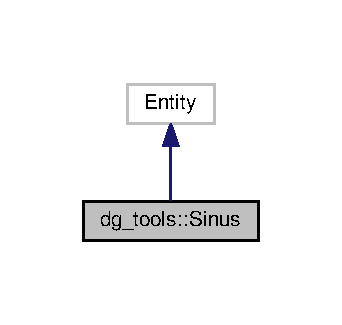
\includegraphics[width=164pt]{classdg__tools_1_1Sinus__inherit__graph}
\end{center}
\end{figure}


Collaboration diagram for dg\+\_\+tools\+:\+:Sinus\+:
\nopagebreak
\begin{figure}[H]
\begin{center}
\leavevmode
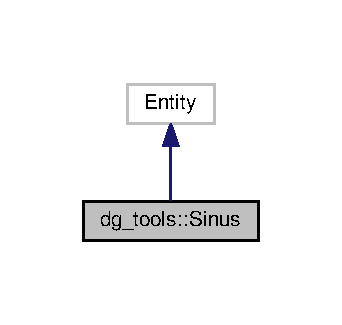
\includegraphics[width=164pt]{classdg__tools_1_1Sinus__coll__graph}
\end{center}
\end{figure}
\subsection*{Public Member Functions}
\begin{DoxyCompactItemize}
\item 
{\bfseries Sinus} (const std\+::string \&name)\hypertarget{classdg__tools_1_1Sinus_a8d140f28cc05cedf44dd759fd19c0d53}{}\label{classdg__tools_1_1Sinus_a8d140f28cc05cedf44dd759fd19c0d53}

\item 
virtual const std\+::string \& {\bfseries get\+Class\+Name} (void) const \hypertarget{classdg__tools_1_1Sinus_ac87645cfb286da4a5b4c3523d69e02c9}{}\label{classdg__tools_1_1Sinus_ac87645cfb286da4a5b4c3523d69e02c9}

\item 
double \& {\bfseries data\+\_\+out\+\_\+callback} (double \&history, int time)\hypertarget{classdg__tools_1_1Sinus_a6148a36649f568751563d52e09687459}{}\label{classdg__tools_1_1Sinus_a6148a36649f568751563d52e09687459}

\end{DoxyCompactItemize}
\subsection*{Public Attributes}
\begin{DoxyCompactItemize}
\item 
dg\+::\+Signal\+Ptr$<$ double, int $>$ {\bfseries data\+\_\+input\+S\+IN}\hypertarget{classdg__tools_1_1Sinus_a0d1afb51099604b472d7cc0029c38f7b}{}\label{classdg__tools_1_1Sinus_a0d1afb51099604b472d7cc0029c38f7b}

\item 
dg\+::\+Signal\+Time\+Dependent$<$ double, int $>$ {\bfseries data\+\_\+out\+S\+O\+UT}\hypertarget{classdg__tools_1_1Sinus_ac0ae9557416fdf0d1afb0a31471e0553}{}\label{classdg__tools_1_1Sinus_ac0ae9557416fdf0d1afb0a31471e0553}

\end{DoxyCompactItemize}
\subsection*{Static Public Attributes}
\begin{DoxyCompactItemize}
\item 
static const std\+::string {\bfseries C\+L\+A\+S\+S\+\_\+\+N\+A\+ME}\hypertarget{classdg__tools_1_1Sinus_ad7933351d7b29f1331f6fad034f16212}{}\label{classdg__tools_1_1Sinus_ad7933351d7b29f1331f6fad034f16212}

\end{DoxyCompactItemize}


\subsection{Detailed Description}
Given input data x, compute y = sin(x). 

The documentation for this class was generated from the following files\+:\begin{DoxyCompactItemize}
\item 
include/dg\+\_\+tools/operator.\+hpp\item 
src/operator.\+cpp\end{DoxyCompactItemize}

\hypertarget{classpython_1_1dg__tools_1_1sliders_1_1Sliders}{}\section{python.\+dg\+\_\+tools.\+sliders.\+Sliders Class Reference}
\label{classpython_1_1dg__tools_1_1sliders_1_1Sliders}\index{python.\+dg\+\_\+tools.\+sliders.\+Sliders@{python.\+dg\+\_\+tools.\+sliders.\+Sliders}}


This class filter the sliders signals from the hardware.  




Inheritance diagram for python.\+dg\+\_\+tools.\+sliders.\+Sliders\+:
\nopagebreak
\begin{figure}[H]
\begin{center}
\leavevmode
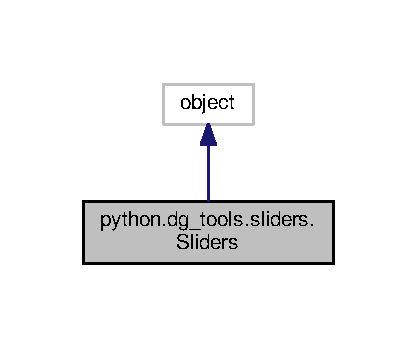
\includegraphics[width=200pt]{classpython_1_1dg__tools_1_1sliders_1_1Sliders__inherit__graph}
\end{center}
\end{figure}


Collaboration diagram for python.\+dg\+\_\+tools.\+sliders.\+Sliders\+:
\nopagebreak
\begin{figure}[H]
\begin{center}
\leavevmode
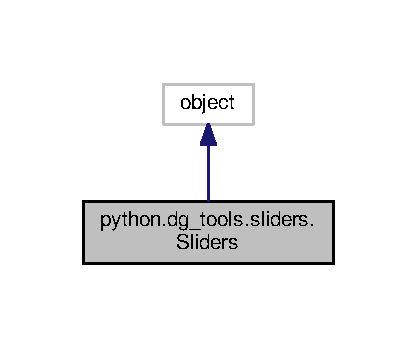
\includegraphics[width=200pt]{classpython_1_1dg__tools_1_1sliders_1_1Sliders__coll__graph}
\end{center}
\end{figure}
\subsection*{Public Member Functions}
\begin{DoxyCompactItemize}
\item 
def \hyperlink{classpython_1_1dg__tools_1_1sliders_1_1Sliders_aba3e1ff7e60f21edd0049e4e049de8c8}{\+\_\+\+\_\+init\+\_\+\+\_\+} (self, nb\+\_\+sliders, prefix=\char`\"{}\char`\"{}, filter\+\_\+size=400, control\+\_\+time\+\_\+step=0.\+001, percentage\+\_\+nyquist\+\_\+cutoff=0.\+1, filter\+\_\+order=6)\hypertarget{classpython_1_1dg__tools_1_1sliders_1_1Sliders_aba3e1ff7e60f21edd0049e4e049de8c8}{}\label{classpython_1_1dg__tools_1_1sliders_1_1Sliders_aba3e1ff7e60f21edd0049e4e049de8c8}

\begin{DoxyCompactList}\small\item\em Initialize the class by creating all the output signals. \end{DoxyCompactList}\item 
def {\bfseries set\+\_\+scale\+\_\+values} (self, scale\+\_\+values)\hypertarget{classpython_1_1dg__tools_1_1sliders_1_1Sliders_a3c0363e583ad2e933888eb4a8cc5b460}{}\label{classpython_1_1dg__tools_1_1sliders_1_1Sliders_a3c0363e583ad2e933888eb4a8cc5b460}

\item 
def {\bfseries set\+\_\+offset\+\_\+values} (self, offset\+\_\+values)\hypertarget{classpython_1_1dg__tools_1_1sliders_1_1Sliders_ad61434524a1855f6b17e8cea010ac25b}{}\label{classpython_1_1dg__tools_1_1sliders_1_1Sliders_ad61434524a1855f6b17e8cea010ac25b}

\item 
def {\bfseries plug\+\_\+slider\+\_\+signal} (self, slider\+\_\+positions\+\_\+sig)\hypertarget{classpython_1_1dg__tools_1_1sliders_1_1Sliders_abf0a53cf4c323c1c1d40d325d7c60953}{}\label{classpython_1_1dg__tools_1_1sliders_1_1Sliders_abf0a53cf4c323c1c1d40d325d7c60953}

\item 
def {\bfseries trace} (self, robot)\hypertarget{classpython_1_1dg__tools_1_1sliders_1_1Sliders_a430660bca42dc72cf68fbc358ee6ba13}{}\label{classpython_1_1dg__tools_1_1sliders_1_1Sliders_a430660bca42dc72cf68fbc358ee6ba13}

\end{DoxyCompactItemize}
\subsection*{Public Attributes}
\begin{DoxyCompactItemize}
\item 
{\bfseries nb\+\_\+sliders}\hypertarget{classpython_1_1dg__tools_1_1sliders_1_1Sliders_aa6e35d118cbd65496ed693771aa41a73}{}\label{classpython_1_1dg__tools_1_1sliders_1_1Sliders_aa6e35d118cbd65496ed693771aa41a73}

\item 
{\bfseries prefix}\hypertarget{classpython_1_1dg__tools_1_1sliders_1_1Sliders_a2b28e317b215914cc78c4ae12d01cd93}{}\label{classpython_1_1dg__tools_1_1sliders_1_1Sliders_a2b28e317b215914cc78c4ae12d01cd93}

\item 
{\bfseries sliders\+\_\+filtered}\hypertarget{classpython_1_1dg__tools_1_1sliders_1_1Sliders_a85047ac2a88c1da44dc1df05434ecb63}{}\label{classpython_1_1dg__tools_1_1sliders_1_1Sliders_a85047ac2a88c1da44dc1df05434ecb63}

\item 
{\bfseries sin}\hypertarget{classpython_1_1dg__tools_1_1sliders_1_1Sliders_a4ecb50f7c4cf17aef714880d516db213}{}\label{classpython_1_1dg__tools_1_1sliders_1_1Sliders_a4ecb50f7c4cf17aef714880d516db213}

\end{DoxyCompactItemize}


\subsection{Detailed Description}
This class filter the sliders signals from the hardware. 

The documentation for this class was generated from the following file\+:\begin{DoxyCompactItemize}
\item 
python/dg\+\_\+tools/sliders.\+py\end{DoxyCompactItemize}

\hypertarget{classpython_1_1dg__tools_1_1leg__impedance__control_1_1solo12__impedance__controller_1_1Solo12ComController}{}\section{python.\+dg\+\_\+tools.\+leg\+\_\+impedance\+\_\+control.\+solo12\+\_\+impedance\+\_\+controller.\+Solo12\+Com\+Controller Class Reference}
\label{classpython_1_1dg__tools_1_1leg__impedance__control_1_1solo12__impedance__controller_1_1Solo12ComController}\index{python.\+dg\+\_\+tools.\+leg\+\_\+impedance\+\_\+control.\+solo12\+\_\+impedance\+\_\+controller.\+Solo12\+Com\+Controller@{python.\+dg\+\_\+tools.\+leg\+\_\+impedance\+\_\+control.\+solo12\+\_\+impedance\+\_\+controller.\+Solo12\+Com\+Controller}}


Inheritance diagram for python.\+dg\+\_\+tools.\+leg\+\_\+impedance\+\_\+control.\+solo12\+\_\+impedance\+\_\+controller.\+Solo12\+Com\+Controller\+:
\nopagebreak
\begin{figure}[H]
\begin{center}
\leavevmode
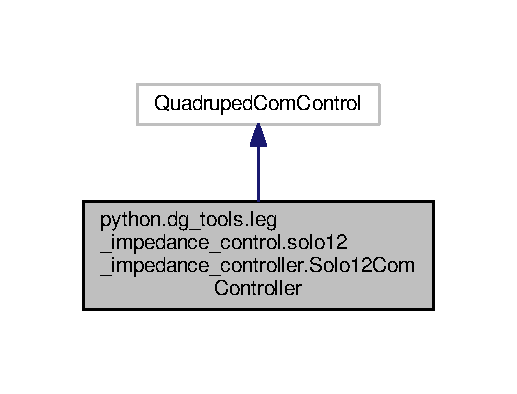
\includegraphics[width=248pt]{classpython_1_1dg__tools_1_1leg__impedance__control_1_1solo12__impedance__controller_1_1Solo12ComController__inherit__graph}
\end{center}
\end{figure}


Collaboration diagram for python.\+dg\+\_\+tools.\+leg\+\_\+impedance\+\_\+control.\+solo12\+\_\+impedance\+\_\+controller.\+Solo12\+Com\+Controller\+:
\nopagebreak
\begin{figure}[H]
\begin{center}
\leavevmode
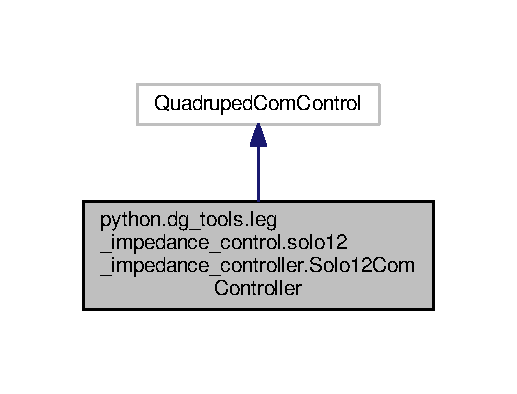
\includegraphics[width=248pt]{classpython_1_1dg__tools_1_1leg__impedance__control_1_1solo12__impedance__controller_1_1Solo12ComController__coll__graph}
\end{center}
\end{figure}
\subsection*{Public Member Functions}
\begin{DoxyCompactItemize}
\item 
def {\bfseries init\+\_\+robot\+\_\+properties} (self)\hypertarget{classpython_1_1dg__tools_1_1leg__impedance__control_1_1solo12__impedance__controller_1_1Solo12ComController_aa7773494f8f24198a332ad0552332ca8}{}\label{classpython_1_1dg__tools_1_1leg__impedance__control_1_1solo12__impedance__controller_1_1Solo12ComController_aa7773494f8f24198a332ad0552332ca8}

\item 
def \hyperlink{classpython_1_1dg__tools_1_1leg__impedance__control_1_1solo12__impedance__controller_1_1Solo12ComController_a386f7ccf7b6fc883ca4f9ca361283ff1}{track\+\_\+com} (self)\hypertarget{classpython_1_1dg__tools_1_1leg__impedance__control_1_1solo12__impedance__controller_1_1Solo12ComController_a386f7ccf7b6fc883ca4f9ca361283ff1}{}\label{classpython_1_1dg__tools_1_1leg__impedance__control_1_1solo12__impedance__controller_1_1Solo12ComController_a386f7ccf7b6fc883ca4f9ca361283ff1}

\begin{DoxyCompactList}\small\item\em Instead of tracking the biased base position and velocity, track the biased com and vcom position. \end{DoxyCompactList}\item 
def {\bfseries record\+\_\+data} (self)\hypertarget{classpython_1_1dg__tools_1_1leg__impedance__control_1_1solo12__impedance__controller_1_1Solo12ComController_a4d8870b7a2d8e41ad92b2147c456656f}{}\label{classpython_1_1dg__tools_1_1leg__impedance__control_1_1solo12__impedance__controller_1_1Solo12ComController_a4d8870b7a2d8e41ad92b2147c456656f}

\item 
def \hyperlink{classpython_1_1dg__tools_1_1leg__impedance__control_1_1solo12__impedance__controller_1_1Solo12ComController_a6791d1b7bbdcca3859cb85358822bb07}{return\+\_\+com\+\_\+torques} (self, args, kwargs)
\end{DoxyCompactItemize}
\subsection*{Public Attributes}
\begin{DoxyCompactItemize}
\item 
{\bfseries robot\+\_\+vicon\+\_\+name}\hypertarget{classpython_1_1dg__tools_1_1leg__impedance__control_1_1solo12__impedance__controller_1_1Solo12ComController_ace0ee7e179807ba79a56934d7b59e217}{}\label{classpython_1_1dg__tools_1_1leg__impedance__control_1_1solo12__impedance__controller_1_1Solo12ComController_ace0ee7e179807ba79a56934d7b59e217}

\item 
{\bfseries robot\+\_\+mass}\hypertarget{classpython_1_1dg__tools_1_1leg__impedance__control_1_1solo12__impedance__controller_1_1Solo12ComController_ad70a7f80bba4d02ae10de3120e707160}{}\label{classpython_1_1dg__tools_1_1leg__impedance__control_1_1solo12__impedance__controller_1_1Solo12ComController_ad70a7f80bba4d02ae10de3120e707160}

\item 
{\bfseries robot\+\_\+base\+\_\+inertia}\hypertarget{classpython_1_1dg__tools_1_1leg__impedance__control_1_1solo12__impedance__controller_1_1Solo12ComController_a6b1c48613a8203b4f0570e1f68e34623}{}\label{classpython_1_1dg__tools_1_1leg__impedance__control_1_1solo12__impedance__controller_1_1Solo12ComController_a6b1c48613a8203b4f0570e1f68e34623}

\item 
{\bfseries robot\+\_\+pin}\hypertarget{classpython_1_1dg__tools_1_1leg__impedance__control_1_1solo12__impedance__controller_1_1Solo12ComController_a42fa317b51400e7b913ef630f78c22ba}{}\label{classpython_1_1dg__tools_1_1leg__impedance__control_1_1solo12__impedance__controller_1_1Solo12ComController_a42fa317b51400e7b913ef630f78c22ba}

\item 
{\bfseries robot\+\_\+dg}\hypertarget{classpython_1_1dg__tools_1_1leg__impedance__control_1_1solo12__impedance__controller_1_1Solo12ComController_a5ef9467a3fbeb3db16fa2ef62c8e54ac}{}\label{classpython_1_1dg__tools_1_1leg__impedance__control_1_1solo12__impedance__controller_1_1Solo12ComController_a5ef9467a3fbeb3db16fa2ef62c8e54ac}

\item 
{\bfseries robot\+\_\+position}\hypertarget{classpython_1_1dg__tools_1_1leg__impedance__control_1_1solo12__impedance__controller_1_1Solo12ComController_a8afc141b6cddfaaeda52454e4cd51e25}{}\label{classpython_1_1dg__tools_1_1leg__impedance__control_1_1solo12__impedance__controller_1_1Solo12ComController_a8afc141b6cddfaaeda52454e4cd51e25}

\item 
{\bfseries robot\+\_\+velocity}\hypertarget{classpython_1_1dg__tools_1_1leg__impedance__control_1_1solo12__impedance__controller_1_1Solo12ComController_a5430b78f98c1ab5f303eb844b0c8dc05}{}\label{classpython_1_1dg__tools_1_1leg__impedance__control_1_1solo12__impedance__controller_1_1Solo12ComController_a5430b78f98c1ab5f303eb844b0c8dc05}

\item 
{\bfseries robot\+\_\+com}\hypertarget{classpython_1_1dg__tools_1_1leg__impedance__control_1_1solo12__impedance__controller_1_1Solo12ComController_a39bbcebb28650b3e9d350a31fcbef1ea}{}\label{classpython_1_1dg__tools_1_1leg__impedance__control_1_1solo12__impedance__controller_1_1Solo12ComController_a39bbcebb28650b3e9d350a31fcbef1ea}

\item 
{\bfseries robot\+\_\+vcom}\hypertarget{classpython_1_1dg__tools_1_1leg__impedance__control_1_1solo12__impedance__controller_1_1Solo12ComController_a52edd425b4c7f9ecea9d8e3949b80f83}{}\label{classpython_1_1dg__tools_1_1leg__impedance__control_1_1solo12__impedance__controller_1_1Solo12ComController_a52edd425b4c7f9ecea9d8e3949b80f83}

\end{DoxyCompactItemize}


\subsection{Member Function Documentation}
\index{python\+::dg\+\_\+tools\+::leg\+\_\+impedance\+\_\+control\+::solo12\+\_\+impedance\+\_\+controller\+::\+Solo12\+Com\+Controller@{python\+::dg\+\_\+tools\+::leg\+\_\+impedance\+\_\+control\+::solo12\+\_\+impedance\+\_\+controller\+::\+Solo12\+Com\+Controller}!return\+\_\+com\+\_\+torques@{return\+\_\+com\+\_\+torques}}
\index{return\+\_\+com\+\_\+torques@{return\+\_\+com\+\_\+torques}!python\+::dg\+\_\+tools\+::leg\+\_\+impedance\+\_\+control\+::solo12\+\_\+impedance\+\_\+controller\+::\+Solo12\+Com\+Controller@{python\+::dg\+\_\+tools\+::leg\+\_\+impedance\+\_\+control\+::solo12\+\_\+impedance\+\_\+controller\+::\+Solo12\+Com\+Controller}}
\subsubsection[{\texorpdfstring{return\+\_\+com\+\_\+torques(self, args, kwargs)}{return_com_torques(self, args, kwargs)}}]{\setlength{\rightskip}{0pt plus 5cm}def python.\+dg\+\_\+tools.\+leg\+\_\+impedance\+\_\+control.\+solo12\+\_\+impedance\+\_\+controller.\+Solo12\+Com\+Controller.\+return\+\_\+com\+\_\+torques (
\begin{DoxyParamCaption}
\item[{}]{self, }
\item[{}]{args, }
\item[{}]{kwargs}
\end{DoxyParamCaption}
)}\hypertarget{classpython_1_1dg__tools_1_1leg__impedance__control_1_1solo12__impedance__controller_1_1Solo12ComController_a6791d1b7bbdcca3859cb85358822bb07}{}\label{classpython_1_1dg__tools_1_1leg__impedance__control_1_1solo12__impedance__controller_1_1Solo12ComController_a6791d1b7bbdcca3859cb85358822bb07}
\begin{DoxyReturn}{Returns}
12-\/dim vector with forces at each endeffector. 
\end{DoxyReturn}


The documentation for this class was generated from the following file\+:\begin{DoxyCompactItemize}
\item 
python/dg\+\_\+tools/leg\+\_\+impedance\+\_\+control/\hyperlink{solo12__impedance__controller_8py}{solo12\+\_\+impedance\+\_\+controller.\+py}\end{DoxyCompactItemize}

\hypertarget{classpython_1_1dg__tools_1_1leg__impedance__control_1_1solo12__impedance__controller_1_1Solo12ImpedanceController}{}\section{python.\+dg\+\_\+tools.\+leg\+\_\+impedance\+\_\+control.\+solo12\+\_\+impedance\+\_\+controller.\+Solo12\+Impedance\+Controller Class Reference}
\label{classpython_1_1dg__tools_1_1leg__impedance__control_1_1solo12__impedance__controller_1_1Solo12ImpedanceController}\index{python.\+dg\+\_\+tools.\+leg\+\_\+impedance\+\_\+control.\+solo12\+\_\+impedance\+\_\+controller.\+Solo12\+Impedance\+Controller@{python.\+dg\+\_\+tools.\+leg\+\_\+impedance\+\_\+control.\+solo12\+\_\+impedance\+\_\+controller.\+Solo12\+Impedance\+Controller}}


Implements leg impedance controller for the solo12 robot.  




Inheritance diagram for python.\+dg\+\_\+tools.\+leg\+\_\+impedance\+\_\+control.\+solo12\+\_\+impedance\+\_\+controller.\+Solo12\+Impedance\+Controller\+:
\nopagebreak
\begin{figure}[H]
\begin{center}
\leavevmode
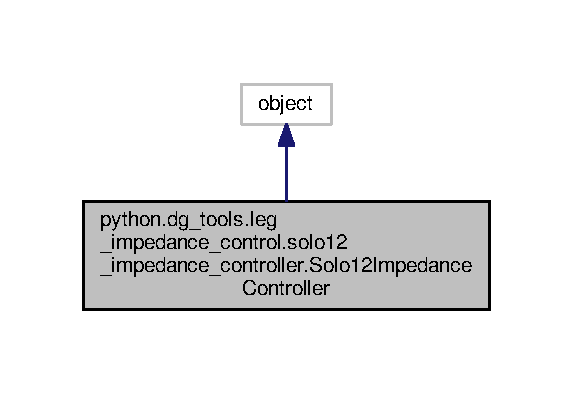
\includegraphics[width=275pt]{classpython_1_1dg__tools_1_1leg__impedance__control_1_1solo12__impedance__controller_1_1Solo12Imda4a48357e96f8799187e352a04853a3}
\end{center}
\end{figure}


Collaboration diagram for python.\+dg\+\_\+tools.\+leg\+\_\+impedance\+\_\+control.\+solo12\+\_\+impedance\+\_\+controller.\+Solo12\+Impedance\+Controller\+:
\nopagebreak
\begin{figure}[H]
\begin{center}
\leavevmode
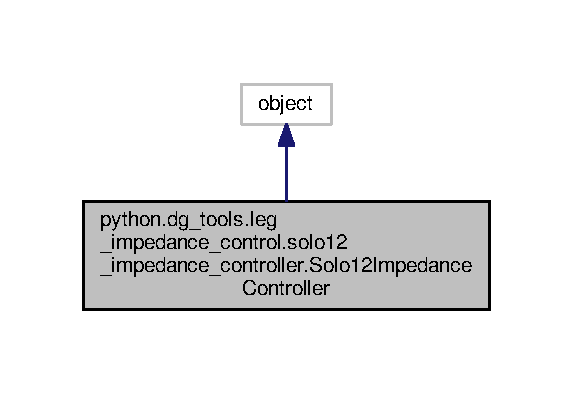
\includegraphics[width=275pt]{classpython_1_1dg__tools_1_1leg__impedance__control_1_1solo12__impedance__controller_1_1Solo12ImpedanceController__coll__graph}
\end{center}
\end{figure}
\subsection*{Public Member Functions}
\begin{DoxyCompactItemize}
\item 
def {\bfseries \+\_\+\+\_\+init\+\_\+\+\_\+} (self, robot)\hypertarget{classpython_1_1dg__tools_1_1leg__impedance__control_1_1solo12__impedance__controller_1_1Solo12ImpedanceController_ad976e804c2d37f15fae274ff6647fb1d}{}\label{classpython_1_1dg__tools_1_1leg__impedance__control_1_1solo12__impedance__controller_1_1Solo12ImpedanceController_ad976e804c2d37f15fae274ff6647fb1d}

\item 
def \hyperlink{classpython_1_1dg__tools_1_1leg__impedance__control_1_1solo12__impedance__controller_1_1Solo12ImpedanceController_a017fe788183d6d226ac80c5857633158}{compute\+\_\+control\+\_\+torques} (self, kp, des\+\_\+pos, kd=None, des\+\_\+vel=None, kf=None, fff=None, base\+\_\+position=None, base\+\_\+velocity=None, pos\+\_\+global=False)
\begin{DoxyCompactList}\small\item\em Computes the desired joint torques for desired configuration using impedance controller. \end{DoxyCompactList}\item 
def \hyperlink{classpython_1_1dg__tools_1_1leg__impedance__control_1_1solo12__impedance__controller_1_1Solo12ImpedanceController_ac3f58073543cac89ec91bccb0e4ab680}{compute\+\_\+com\+\_\+end\+\_\+eff\+\_\+pos} (self)
\begin{DoxyCompactList}\small\item\em Returns the endeffector positions wrt com position in world frame. \end{DoxyCompactList}\item 
def \hyperlink{classpython_1_1dg__tools_1_1leg__impedance__control_1_1solo12__impedance__controller_1_1Solo12ImpedanceController_a4c2e260a3a8750f9490763a74d139788}{compute\+\_\+abs\+\_\+end\+\_\+eff\+\_\+pos} (self)
\begin{DoxyCompactList}\small\item\em Returns the endeffector positions wrt world frame. \end{DoxyCompactList}\item 
def \hyperlink{classpython_1_1dg__tools_1_1leg__impedance__control_1_1solo12__impedance__controller_1_1Solo12ImpedanceController_aeac195c145f446cf632b10e6390c667e}{compute\+\_\+abs\+\_\+end\+\_\+eff\+\_\+vel} (self)
\begin{DoxyCompactList}\small\item\em Returns the endeffector velocity signal. \end{DoxyCompactList}\item 
def {\bfseries record\+\_\+data} (self)\hypertarget{classpython_1_1dg__tools_1_1leg__impedance__control_1_1solo12__impedance__controller_1_1Solo12ImpedanceController_a3ed90b4a3ce54d255263e07f9892bff5}{}\label{classpython_1_1dg__tools_1_1leg__impedance__control_1_1solo12__impedance__controller_1_1Solo12ImpedanceController_a3ed90b4a3ce54d255263e07f9892bff5}

\end{DoxyCompactItemize}
\subsection*{Public Attributes}
\begin{DoxyCompactItemize}
\item 
{\bfseries robot}\hypertarget{classpython_1_1dg__tools_1_1leg__impedance__control_1_1solo12__impedance__controller_1_1Solo12ImpedanceController_aa73fbab5b26fe8f2a75f92aaebf30989}{}\label{classpython_1_1dg__tools_1_1leg__impedance__control_1_1solo12__impedance__controller_1_1Solo12ImpedanceController_aa73fbab5b26fe8f2a75f92aaebf30989}

\item 
{\bfseries leg\+\_\+imp\+\_\+ctrl}\hypertarget{classpython_1_1dg__tools_1_1leg__impedance__control_1_1solo12__impedance__controller_1_1Solo12ImpedanceController_a01f435dd61d4098d1c805a6e558be4b4}{}\label{classpython_1_1dg__tools_1_1leg__impedance__control_1_1solo12__impedance__controller_1_1Solo12ImpedanceController_a01f435dd61d4098d1c805a6e558be4b4}

\item 
{\bfseries leg\+\_\+idx}\hypertarget{classpython_1_1dg__tools_1_1leg__impedance__control_1_1solo12__impedance__controller_1_1Solo12ImpedanceController_a771da81c0a0bd6853be6c2aa2cdbf568}{}\label{classpython_1_1dg__tools_1_1leg__impedance__control_1_1solo12__impedance__controller_1_1Solo12ImpedanceController_a771da81c0a0bd6853be6c2aa2cdbf568}

\item 
{\bfseries abs\+\_\+end\+\_\+eff\+\_\+pos}\hypertarget{classpython_1_1dg__tools_1_1leg__impedance__control_1_1solo12__impedance__controller_1_1Solo12ImpedanceController_a0ed38547e9f0e814964e9fdef989e09c}{}\label{classpython_1_1dg__tools_1_1leg__impedance__control_1_1solo12__impedance__controller_1_1Solo12ImpedanceController_a0ed38547e9f0e814964e9fdef989e09c}

\item 
{\bfseries abs\+\_\+end\+\_\+eff\+\_\+vel}\hypertarget{classpython_1_1dg__tools_1_1leg__impedance__control_1_1solo12__impedance__controller_1_1Solo12ImpedanceController_af260596a80b7d4c68bf58201e79f0ce3}{}\label{classpython_1_1dg__tools_1_1leg__impedance__control_1_1solo12__impedance__controller_1_1Solo12ImpedanceController_af260596a80b7d4c68bf58201e79f0ce3}

\item 
{\bfseries com\+\_\+end\+\_\+eff\+\_\+pos}\hypertarget{classpython_1_1dg__tools_1_1leg__impedance__control_1_1solo12__impedance__controller_1_1Solo12ImpedanceController_a835e5c02a065b87bf50d9496d79c6a3e}{}\label{classpython_1_1dg__tools_1_1leg__impedance__control_1_1solo12__impedance__controller_1_1Solo12ImpedanceController_a835e5c02a065b87bf50d9496d79c6a3e}

\item 
{\bfseries des\+\_\+pos}\hypertarget{classpython_1_1dg__tools_1_1leg__impedance__control_1_1solo12__impedance__controller_1_1Solo12ImpedanceController_a6b24d28f6d0daee671680f6a9ca06c73}{}\label{classpython_1_1dg__tools_1_1leg__impedance__control_1_1solo12__impedance__controller_1_1Solo12ImpedanceController_a6b24d28f6d0daee671680f6a9ca06c73}

\item 
{\bfseries des\+\_\+vel}\hypertarget{classpython_1_1dg__tools_1_1leg__impedance__control_1_1solo12__impedance__controller_1_1Solo12ImpedanceController_aadba49bed9d2b7ab71fee7db275a5ef2}{}\label{classpython_1_1dg__tools_1_1leg__impedance__control_1_1solo12__impedance__controller_1_1Solo12ImpedanceController_aadba49bed9d2b7ab71fee7db275a5ef2}

\item 
{\bfseries fff}\hypertarget{classpython_1_1dg__tools_1_1leg__impedance__control_1_1solo12__impedance__controller_1_1Solo12ImpedanceController_a286eed471a547c5a48928be53f66d8f6}{}\label{classpython_1_1dg__tools_1_1leg__impedance__control_1_1solo12__impedance__controller_1_1Solo12ImpedanceController_a286eed471a547c5a48928be53f66d8f6}

\item 
{\bfseries joint\+\_\+positions}\hypertarget{classpython_1_1dg__tools_1_1leg__impedance__control_1_1solo12__impedance__controller_1_1Solo12ImpedanceController_abb1c09464c619c757a96eaccfed882ab}{}\label{classpython_1_1dg__tools_1_1leg__impedance__control_1_1solo12__impedance__controller_1_1Solo12ImpedanceController_abb1c09464c619c757a96eaccfed882ab}

\item 
{\bfseries joint\+\_\+velocities}\hypertarget{classpython_1_1dg__tools_1_1leg__impedance__control_1_1solo12__impedance__controller_1_1Solo12ImpedanceController_ac12f110e06e2e55a7a8e154e016e7373}{}\label{classpython_1_1dg__tools_1_1leg__impedance__control_1_1solo12__impedance__controller_1_1Solo12ImpedanceController_ac12f110e06e2e55a7a8e154e016e7373}

\item 
{\bfseries robot\+\_\+position}\hypertarget{classpython_1_1dg__tools_1_1leg__impedance__control_1_1solo12__impedance__controller_1_1Solo12ImpedanceController_a3790cf52b324522282dcebd2109c9476}{}\label{classpython_1_1dg__tools_1_1leg__impedance__control_1_1solo12__impedance__controller_1_1Solo12ImpedanceController_a3790cf52b324522282dcebd2109c9476}

\item 
{\bfseries robot\+\_\+velocity}\hypertarget{classpython_1_1dg__tools_1_1leg__impedance__control_1_1solo12__impedance__controller_1_1Solo12ImpedanceController_a1c8c714517fc4d36a177643d161add7d}{}\label{classpython_1_1dg__tools_1_1leg__impedance__control_1_1solo12__impedance__controller_1_1Solo12ImpedanceController_a1c8c714517fc4d36a177643d161add7d}

\item 
{\bfseries control\+\_\+torques}\hypertarget{classpython_1_1dg__tools_1_1leg__impedance__control_1_1solo12__impedance__controller_1_1Solo12ImpedanceController_ae2ef4d7e7f38bce53b931a5d820be71b}{}\label{classpython_1_1dg__tools_1_1leg__impedance__control_1_1solo12__impedance__controller_1_1Solo12ImpedanceController_ae2ef4d7e7f38bce53b931a5d820be71b}

\end{DoxyCompactItemize}
\subsection*{Private Member Functions}
\begin{DoxyCompactItemize}
\item 
def {\bfseries \+\_\+compute\+\_\+leg\+\_\+control\+\_\+torques} (self, leg\+\_\+idx, kp, kd, kf, des\+\_\+pos, des\+\_\+vel, fff)\hypertarget{classpython_1_1dg__tools_1_1leg__impedance__control_1_1solo12__impedance__controller_1_1Solo12ImpedanceController_a75cd13cf011b08ff89edf2342b6fcf38}{}\label{classpython_1_1dg__tools_1_1leg__impedance__control_1_1solo12__impedance__controller_1_1Solo12ImpedanceController_a75cd13cf011b08ff89edf2342b6fcf38}

\item 
def \hyperlink{classpython_1_1dg__tools_1_1leg__impedance__control_1_1solo12__impedance__controller_1_1Solo12ImpedanceController_a0782f26b37ab4ada7b2443685975a673}{\+\_\+slice\+\_\+vec} (self, vec, leg\+\_\+idx, name)
\begin{DoxyCompactList}\small\item\em Helper for slicing the desired vector for a leg. \end{DoxyCompactList}\end{DoxyCompactItemize}


\subsection{Detailed Description}
Implements leg impedance controller for the solo12 robot. 

Compared to the solo8 implementation, this uses the full solo12 urdf. Especially, it computes the desired torque at the actual legs instead of using the same \char`\"{}teststand\char`\"{} leg at each joint. 

\subsection{Member Function Documentation}
\index{python\+::dg\+\_\+tools\+::leg\+\_\+impedance\+\_\+control\+::solo12\+\_\+impedance\+\_\+controller\+::\+Solo12\+Impedance\+Controller@{python\+::dg\+\_\+tools\+::leg\+\_\+impedance\+\_\+control\+::solo12\+\_\+impedance\+\_\+controller\+::\+Solo12\+Impedance\+Controller}!\+\_\+slice\+\_\+vec@{\+\_\+slice\+\_\+vec}}
\index{\+\_\+slice\+\_\+vec@{\+\_\+slice\+\_\+vec}!python\+::dg\+\_\+tools\+::leg\+\_\+impedance\+\_\+control\+::solo12\+\_\+impedance\+\_\+controller\+::\+Solo12\+Impedance\+Controller@{python\+::dg\+\_\+tools\+::leg\+\_\+impedance\+\_\+control\+::solo12\+\_\+impedance\+\_\+controller\+::\+Solo12\+Impedance\+Controller}}
\subsubsection[{\texorpdfstring{\+\_\+slice\+\_\+vec(self, vec, leg\+\_\+idx, name)}{_slice_vec(self, vec, leg_idx, name)}}]{\setlength{\rightskip}{0pt plus 5cm}def python.\+dg\+\_\+tools.\+leg\+\_\+impedance\+\_\+control.\+solo12\+\_\+impedance\+\_\+controller.\+Solo12\+Impedance\+Controller.\+\_\+slice\+\_\+vec (
\begin{DoxyParamCaption}
\item[{}]{self, }
\item[{}]{vec, }
\item[{}]{leg\+\_\+idx, }
\item[{}]{name}
\end{DoxyParamCaption}
)\hspace{0.3cm}{\ttfamily [private]}}\hypertarget{classpython_1_1dg__tools_1_1leg__impedance__control_1_1solo12__impedance__controller_1_1Solo12ImpedanceController_a0782f26b37ab4ada7b2443685975a673}{}\label{classpython_1_1dg__tools_1_1leg__impedance__control_1_1solo12__impedance__controller_1_1Solo12ImpedanceController_a0782f26b37ab4ada7b2443685975a673}


Helper for slicing the desired vector for a leg. 


\begin{DoxyParams}{Parameters}
{\em vec} & (1$\ast$12 vector or None) Vector to slice for a given leg \\
\hline
{\em leg\+\_\+idx} & (int) Leg index to slice the vector for \\
\hline
{\em name} & (str) Name for the slicing operator to use.\\
\hline
\end{DoxyParams}
\begin{DoxyReturn}{Returns}
1$\ast$3 vector slice for the leg, None if vec was None. 
\end{DoxyReturn}
\index{python\+::dg\+\_\+tools\+::leg\+\_\+impedance\+\_\+control\+::solo12\+\_\+impedance\+\_\+controller\+::\+Solo12\+Impedance\+Controller@{python\+::dg\+\_\+tools\+::leg\+\_\+impedance\+\_\+control\+::solo12\+\_\+impedance\+\_\+controller\+::\+Solo12\+Impedance\+Controller}!compute\+\_\+abs\+\_\+end\+\_\+eff\+\_\+pos@{compute\+\_\+abs\+\_\+end\+\_\+eff\+\_\+pos}}
\index{compute\+\_\+abs\+\_\+end\+\_\+eff\+\_\+pos@{compute\+\_\+abs\+\_\+end\+\_\+eff\+\_\+pos}!python\+::dg\+\_\+tools\+::leg\+\_\+impedance\+\_\+control\+::solo12\+\_\+impedance\+\_\+controller\+::\+Solo12\+Impedance\+Controller@{python\+::dg\+\_\+tools\+::leg\+\_\+impedance\+\_\+control\+::solo12\+\_\+impedance\+\_\+controller\+::\+Solo12\+Impedance\+Controller}}
\subsubsection[{\texorpdfstring{compute\+\_\+abs\+\_\+end\+\_\+eff\+\_\+pos(self)}{compute_abs_end_eff_pos(self)}}]{\setlength{\rightskip}{0pt plus 5cm}def python.\+dg\+\_\+tools.\+leg\+\_\+impedance\+\_\+control.\+solo12\+\_\+impedance\+\_\+controller.\+Solo12\+Impedance\+Controller.\+compute\+\_\+abs\+\_\+end\+\_\+eff\+\_\+pos (
\begin{DoxyParamCaption}
\item[{}]{self}
\end{DoxyParamCaption}
)}\hypertarget{classpython_1_1dg__tools_1_1leg__impedance__control_1_1solo12__impedance__controller_1_1Solo12ImpedanceController_a4c2e260a3a8750f9490763a74d139788}{}\label{classpython_1_1dg__tools_1_1leg__impedance__control_1_1solo12__impedance__controller_1_1Solo12ImpedanceController_a4c2e260a3a8750f9490763a74d139788}


Returns the endeffector positions wrt world frame. 

\begin{DoxyReturn}{Returns}
Signal$<$dg\+::\+Vector, size=12$>$ Stack of the four endeffector positions 
\end{DoxyReturn}
\index{python\+::dg\+\_\+tools\+::leg\+\_\+impedance\+\_\+control\+::solo12\+\_\+impedance\+\_\+controller\+::\+Solo12\+Impedance\+Controller@{python\+::dg\+\_\+tools\+::leg\+\_\+impedance\+\_\+control\+::solo12\+\_\+impedance\+\_\+controller\+::\+Solo12\+Impedance\+Controller}!compute\+\_\+abs\+\_\+end\+\_\+eff\+\_\+vel@{compute\+\_\+abs\+\_\+end\+\_\+eff\+\_\+vel}}
\index{compute\+\_\+abs\+\_\+end\+\_\+eff\+\_\+vel@{compute\+\_\+abs\+\_\+end\+\_\+eff\+\_\+vel}!python\+::dg\+\_\+tools\+::leg\+\_\+impedance\+\_\+control\+::solo12\+\_\+impedance\+\_\+controller\+::\+Solo12\+Impedance\+Controller@{python\+::dg\+\_\+tools\+::leg\+\_\+impedance\+\_\+control\+::solo12\+\_\+impedance\+\_\+controller\+::\+Solo12\+Impedance\+Controller}}
\subsubsection[{\texorpdfstring{compute\+\_\+abs\+\_\+end\+\_\+eff\+\_\+vel(self)}{compute_abs_end_eff_vel(self)}}]{\setlength{\rightskip}{0pt plus 5cm}def python.\+dg\+\_\+tools.\+leg\+\_\+impedance\+\_\+control.\+solo12\+\_\+impedance\+\_\+controller.\+Solo12\+Impedance\+Controller.\+compute\+\_\+abs\+\_\+end\+\_\+eff\+\_\+vel (
\begin{DoxyParamCaption}
\item[{}]{self}
\end{DoxyParamCaption}
)}\hypertarget{classpython_1_1dg__tools_1_1leg__impedance__control_1_1solo12__impedance__controller_1_1Solo12ImpedanceController_aeac195c145f446cf632b10e6390c667e}{}\label{classpython_1_1dg__tools_1_1leg__impedance__control_1_1solo12__impedance__controller_1_1Solo12ImpedanceController_aeac195c145f446cf632b10e6390c667e}


Returns the endeffector velocity signal. 

\index{python\+::dg\+\_\+tools\+::leg\+\_\+impedance\+\_\+control\+::solo12\+\_\+impedance\+\_\+controller\+::\+Solo12\+Impedance\+Controller@{python\+::dg\+\_\+tools\+::leg\+\_\+impedance\+\_\+control\+::solo12\+\_\+impedance\+\_\+controller\+::\+Solo12\+Impedance\+Controller}!compute\+\_\+com\+\_\+end\+\_\+eff\+\_\+pos@{compute\+\_\+com\+\_\+end\+\_\+eff\+\_\+pos}}
\index{compute\+\_\+com\+\_\+end\+\_\+eff\+\_\+pos@{compute\+\_\+com\+\_\+end\+\_\+eff\+\_\+pos}!python\+::dg\+\_\+tools\+::leg\+\_\+impedance\+\_\+control\+::solo12\+\_\+impedance\+\_\+controller\+::\+Solo12\+Impedance\+Controller@{python\+::dg\+\_\+tools\+::leg\+\_\+impedance\+\_\+control\+::solo12\+\_\+impedance\+\_\+controller\+::\+Solo12\+Impedance\+Controller}}
\subsubsection[{\texorpdfstring{compute\+\_\+com\+\_\+end\+\_\+eff\+\_\+pos(self)}{compute_com_end_eff_pos(self)}}]{\setlength{\rightskip}{0pt plus 5cm}def python.\+dg\+\_\+tools.\+leg\+\_\+impedance\+\_\+control.\+solo12\+\_\+impedance\+\_\+controller.\+Solo12\+Impedance\+Controller.\+compute\+\_\+com\+\_\+end\+\_\+eff\+\_\+pos (
\begin{DoxyParamCaption}
\item[{}]{self}
\end{DoxyParamCaption}
)}\hypertarget{classpython_1_1dg__tools_1_1leg__impedance__control_1_1solo12__impedance__controller_1_1Solo12ImpedanceController_ac3f58073543cac89ec91bccb0e4ab680}{}\label{classpython_1_1dg__tools_1_1leg__impedance__control_1_1solo12__impedance__controller_1_1Solo12ImpedanceController_ac3f58073543cac89ec91bccb0e4ab680}


Returns the endeffector positions wrt com position in world frame. 

\begin{DoxyReturn}{Returns}
Signal$<$dg\+::\+Vector, size=12$>$ Stack of the four endeffector positions 
\end{DoxyReturn}
\index{python\+::dg\+\_\+tools\+::leg\+\_\+impedance\+\_\+control\+::solo12\+\_\+impedance\+\_\+controller\+::\+Solo12\+Impedance\+Controller@{python\+::dg\+\_\+tools\+::leg\+\_\+impedance\+\_\+control\+::solo12\+\_\+impedance\+\_\+controller\+::\+Solo12\+Impedance\+Controller}!compute\+\_\+control\+\_\+torques@{compute\+\_\+control\+\_\+torques}}
\index{compute\+\_\+control\+\_\+torques@{compute\+\_\+control\+\_\+torques}!python\+::dg\+\_\+tools\+::leg\+\_\+impedance\+\_\+control\+::solo12\+\_\+impedance\+\_\+controller\+::\+Solo12\+Impedance\+Controller@{python\+::dg\+\_\+tools\+::leg\+\_\+impedance\+\_\+control\+::solo12\+\_\+impedance\+\_\+controller\+::\+Solo12\+Impedance\+Controller}}
\subsubsection[{\texorpdfstring{compute\+\_\+control\+\_\+torques(self, kp, des\+\_\+pos, kd=\+None, des\+\_\+vel=\+None, kf=\+None, fff=\+None, base\+\_\+position=\+None, base\+\_\+velocity=\+None, pos\+\_\+global=\+False)}{compute_control_torques(self, kp, des_pos, kd=None, des_vel=None, kf=None, fff=None, base_position=None, base_velocity=None, pos_global=False)}}]{\setlength{\rightskip}{0pt plus 5cm}def python.\+dg\+\_\+tools.\+leg\+\_\+impedance\+\_\+control.\+solo12\+\_\+impedance\+\_\+controller.\+Solo12\+Impedance\+Controller.\+compute\+\_\+control\+\_\+torques (
\begin{DoxyParamCaption}
\item[{}]{self, }
\item[{}]{kp, }
\item[{}]{des\+\_\+pos, }
\item[{}]{kd = {\ttfamily None}, }
\item[{}]{des\+\_\+vel = {\ttfamily None}, }
\item[{}]{kf = {\ttfamily None}, }
\item[{}]{fff = {\ttfamily None}, }
\item[{}]{base\+\_\+position = {\ttfamily None}, }
\item[{}]{base\+\_\+velocity = {\ttfamily None}, }
\item[{}]{pos\+\_\+global = {\ttfamily False}}
\end{DoxyParamCaption}
)}\hypertarget{classpython_1_1dg__tools_1_1leg__impedance__control_1_1solo12__impedance__controller_1_1Solo12ImpedanceController_a017fe788183d6d226ac80c5857633158}{}\label{classpython_1_1dg__tools_1_1leg__impedance__control_1_1solo12__impedance__controller_1_1Solo12ImpedanceController_a017fe788183d6d226ac80c5857633158}


Computes the desired joint torques for desired configuration using impedance controller. 

If no base position or velocity is provided, assume the base if fixed at the origin.


\begin{DoxyParams}{Parameters}
{\em Kp} & (double) proportional gain (double) \\
\hline
{\em des\+\_\+pos} & (1$\ast$12 vector) desired\+\_\+position in current time step \\
\hline
{\em Kd} & derivative gain (double) \\
\hline
{\em des\+\_\+vel} & (1$\ast$12 vector) desired\+\_\+velocity in current time step \\
\hline
{\em fff} & (1$\ast$12 vector) Feed forward force \\
\hline
{\em base\+\_\+position} & (1$\ast$7 vector, optional) Base position (translation + quaternion) \\
\hline
{\em base\+\_\+velocity} & (1$\ast$6 vector, optional) Base velocity (translation + rotation) \\
\hline
{\em pos\+\_\+global} & If true, track des\+\_\+pos in global frame. Requires base\+\_\+position and base\+\_\+velocity to be set. \\
\hline
\end{DoxyParams}
\begin{DoxyReturn}{Returns}
Final joint torques (1 $\ast$ 12 vector) 
\end{DoxyReturn}


The documentation for this class was generated from the following file\+:\begin{DoxyCompactItemize}
\item 
python/dg\+\_\+tools/leg\+\_\+impedance\+\_\+control/\hyperlink{solo12__impedance__controller_8py}{solo12\+\_\+impedance\+\_\+controller.\+py}\end{DoxyCompactItemize}

\hypertarget{classpython_1_1dg__tools_1_1leg__impedance__control_1_1solo12__impedance__controller_1_1Solo12LegImpedanceController}{}\section{python.\+dg\+\_\+tools.\+leg\+\_\+impedance\+\_\+control.\+solo12\+\_\+impedance\+\_\+controller.\+Solo12\+Leg\+Impedance\+Controller Class Reference}
\label{classpython_1_1dg__tools_1_1leg__impedance__control_1_1solo12__impedance__controller_1_1Solo12LegImpedanceController}\index{python.\+dg\+\_\+tools.\+leg\+\_\+impedance\+\_\+control.\+solo12\+\_\+impedance\+\_\+controller.\+Solo12\+Leg\+Impedance\+Controller@{python.\+dg\+\_\+tools.\+leg\+\_\+impedance\+\_\+control.\+solo12\+\_\+impedance\+\_\+controller.\+Solo12\+Leg\+Impedance\+Controller}}


Impedance controller for single leg on solo12.  




Inheritance diagram for python.\+dg\+\_\+tools.\+leg\+\_\+impedance\+\_\+control.\+solo12\+\_\+impedance\+\_\+controller.\+Solo12\+Leg\+Impedance\+Controller\+:
\nopagebreak
\begin{figure}[H]
\begin{center}
\leavevmode
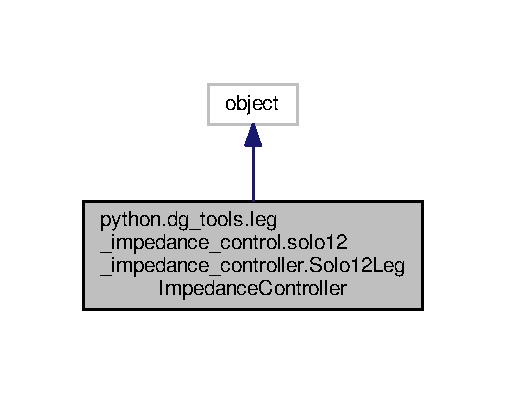
\includegraphics[width=243pt]{classpython_1_1dg__tools_1_1leg__impedance__control_1_1solo12__impedance__controller_1_1Solo12Lef11bf14cfea20afec925052017bf9b7f}
\end{center}
\end{figure}


Collaboration diagram for python.\+dg\+\_\+tools.\+leg\+\_\+impedance\+\_\+control.\+solo12\+\_\+impedance\+\_\+controller.\+Solo12\+Leg\+Impedance\+Controller\+:
\nopagebreak
\begin{figure}[H]
\begin{center}
\leavevmode
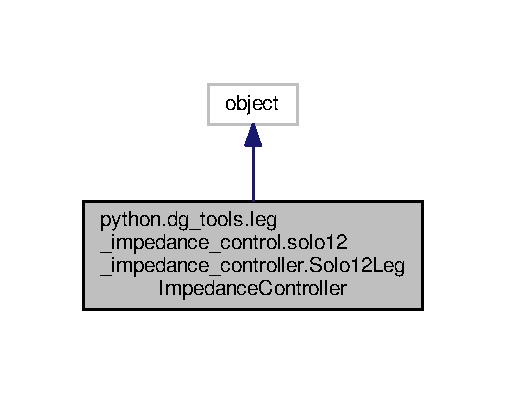
\includegraphics[width=243pt]{classpython_1_1dg__tools_1_1leg__impedance__control_1_1solo12__impedance__controller_1_1Solo12Le6bc9863ffab3fd8e5fa078bb855c3c90}
\end{center}
\end{figure}
\subsection*{Public Member Functions}
\begin{DoxyCompactItemize}
\item 
def \hyperlink{classpython_1_1dg__tools_1_1leg__impedance__control_1_1solo12__impedance__controller_1_1Solo12LegImpedanceController_aa956e758651721d07585b2c1d6f197c7}{\+\_\+\+\_\+init\+\_\+\+\_\+} (self, leg\+\_\+name, joint\+\_\+indices\+\_\+range)
\item 
def {\bfseries compute\+\_\+control\+\_\+torques} (self, kp, kd, kf, des\+\_\+pos, des\+\_\+vel, fff, pos\+\_\+global=False)\hypertarget{classpython_1_1dg__tools_1_1leg__impedance__control_1_1solo12__impedance__controller_1_1Solo12LegImpedanceController_a50833108bac36327c6971e15f4ae8ff5}{}\label{classpython_1_1dg__tools_1_1leg__impedance__control_1_1solo12__impedance__controller_1_1Solo12LegImpedanceController_a50833108bac36327c6971e15f4ae8ff5}

\item 
def {\bfseries record\+\_\+data} (self, robot)\hypertarget{classpython_1_1dg__tools_1_1leg__impedance__control_1_1solo12__impedance__controller_1_1Solo12LegImpedanceController_a4ccf4791677cb4b38c1bd2470f2c1ed4}{}\label{classpython_1_1dg__tools_1_1leg__impedance__control_1_1solo12__impedance__controller_1_1Solo12LegImpedanceController_a4ccf4791677cb4b38c1bd2470f2c1ed4}

\end{DoxyCompactItemize}
\subsection*{Public Attributes}
\begin{DoxyCompactItemize}
\item 
{\bfseries leg\+\_\+name}\hypertarget{classpython_1_1dg__tools_1_1leg__impedance__control_1_1solo12__impedance__controller_1_1Solo12LegImpedanceController_a4cbb793ede6548fefce01df481181429}{}\label{classpython_1_1dg__tools_1_1leg__impedance__control_1_1solo12__impedance__controller_1_1Solo12LegImpedanceController_a4cbb793ede6548fefce01df481181429}

\item 
{\bfseries joint\+\_\+indices\+\_\+range}\hypertarget{classpython_1_1dg__tools_1_1leg__impedance__control_1_1solo12__impedance__controller_1_1Solo12LegImpedanceController_aba15200059ad006bb30d667200bd9635}{}\label{classpython_1_1dg__tools_1_1leg__impedance__control_1_1solo12__impedance__controller_1_1Solo12LegImpedanceController_aba15200059ad006bb30d667200bd9635}

\item 
{\bfseries robot\+\_\+pin}\hypertarget{classpython_1_1dg__tools_1_1leg__impedance__control_1_1solo12__impedance__controller_1_1Solo12LegImpedanceController_aceb6feff2edfbc8d691bb6ce0236ca27}{}\label{classpython_1_1dg__tools_1_1leg__impedance__control_1_1solo12__impedance__controller_1_1Solo12LegImpedanceController_aceb6feff2edfbc8d691bb6ce0236ca27}

\item 
{\bfseries robot\+\_\+dg}\hypertarget{classpython_1_1dg__tools_1_1leg__impedance__control_1_1solo12__impedance__controller_1_1Solo12LegImpedanceController_aa7cfe737d3bd9e103747bcbeff061c27}{}\label{classpython_1_1dg__tools_1_1leg__impedance__control_1_1solo12__impedance__controller_1_1Solo12LegImpedanceController_aa7cfe737d3bd9e103747bcbeff061c27}

\item 
{\bfseries joint\+\_\+positions\+\_\+sin}\hypertarget{classpython_1_1dg__tools_1_1leg__impedance__control_1_1solo12__impedance__controller_1_1Solo12LegImpedanceController_a88f9163d5f8d8868c17309297b86a9b2}{}\label{classpython_1_1dg__tools_1_1leg__impedance__control_1_1solo12__impedance__controller_1_1Solo12LegImpedanceController_a88f9163d5f8d8868c17309297b86a9b2}

\item 
{\bfseries joint\+\_\+velocities\+\_\+sin}\hypertarget{classpython_1_1dg__tools_1_1leg__impedance__control_1_1solo12__impedance__controller_1_1Solo12LegImpedanceController_aa02f5974a5edb985308f96bb6064070e}{}\label{classpython_1_1dg__tools_1_1leg__impedance__control_1_1solo12__impedance__controller_1_1Solo12LegImpedanceController_aa02f5974a5edb985308f96bb6064070e}

\item 
{\bfseries xyzpos\+\_\+hip}\hypertarget{classpython_1_1dg__tools_1_1leg__impedance__control_1_1solo12__impedance__controller_1_1Solo12LegImpedanceController_a94d40e8bf8cf618d860e06ea8f21b080}{}\label{classpython_1_1dg__tools_1_1leg__impedance__control_1_1solo12__impedance__controller_1_1Solo12LegImpedanceController_a94d40e8bf8cf618d860e06ea8f21b080}

\item 
{\bfseries xyzpos\+\_\+foot}\hypertarget{classpython_1_1dg__tools_1_1leg__impedance__control_1_1solo12__impedance__controller_1_1Solo12LegImpedanceController_ac765ed4b0b16d8520f7b908b0c616abe}{}\label{classpython_1_1dg__tools_1_1leg__impedance__control_1_1solo12__impedance__controller_1_1Solo12LegImpedanceController_ac765ed4b0b16d8520f7b908b0c616abe}

\item 
{\bfseries rel\+\_\+pos\+\_\+foot}\hypertarget{classpython_1_1dg__tools_1_1leg__impedance__control_1_1solo12__impedance__controller_1_1Solo12LegImpedanceController_a88a97eb550554d65f6f3648df7b812c5}{}\label{classpython_1_1dg__tools_1_1leg__impedance__control_1_1solo12__impedance__controller_1_1Solo12LegImpedanceController_a88a97eb550554d65f6f3648df7b812c5}

\item 
{\bfseries jacT}\hypertarget{classpython_1_1dg__tools_1_1leg__impedance__control_1_1solo12__impedance__controller_1_1Solo12LegImpedanceController_acb0410734f37d4d64f42bd93673c40bb}{}\label{classpython_1_1dg__tools_1_1leg__impedance__control_1_1solo12__impedance__controller_1_1Solo12LegImpedanceController_acb0410734f37d4d64f42bd93673c40bb}

\item 
{\bfseries rct\+\_\+args}\hypertarget{classpython_1_1dg__tools_1_1leg__impedance__control_1_1solo12__impedance__controller_1_1Solo12LegImpedanceController_a72720a53cc95bbb643591d5c0ab4f12c}{}\label{classpython_1_1dg__tools_1_1leg__impedance__control_1_1solo12__impedance__controller_1_1Solo12LegImpedanceController_a72720a53cc95bbb643591d5c0ab4f12c}

\item 
{\bfseries jac}\hypertarget{classpython_1_1dg__tools_1_1leg__impedance__control_1_1solo12__impedance__controller_1_1Solo12LegImpedanceController_ad2a344961469700abd1d42c0621930bd}{}\label{classpython_1_1dg__tools_1_1leg__impedance__control_1_1solo12__impedance__controller_1_1Solo12LegImpedanceController_ad2a344961469700abd1d42c0621930bd}

\item 
{\bfseries pos\+\_\+error}\hypertarget{classpython_1_1dg__tools_1_1leg__impedance__control_1_1solo12__impedance__controller_1_1Solo12LegImpedanceController_a55a1b776288c42531c2174f5aead3bc6}{}\label{classpython_1_1dg__tools_1_1leg__impedance__control_1_1solo12__impedance__controller_1_1Solo12LegImpedanceController_a55a1b776288c42531c2174f5aead3bc6}

\item 
{\bfseries rel\+\_\+vel\+\_\+foot}\hypertarget{classpython_1_1dg__tools_1_1leg__impedance__control_1_1solo12__impedance__controller_1_1Solo12LegImpedanceController_a70ac9204066939edc30310bfa2c4b086}{}\label{classpython_1_1dg__tools_1_1leg__impedance__control_1_1solo12__impedance__controller_1_1Solo12LegImpedanceController_a70ac9204066939edc30310bfa2c4b086}

\item 
{\bfseries vel\+\_\+error}\hypertarget{classpython_1_1dg__tools_1_1leg__impedance__control_1_1solo12__impedance__controller_1_1Solo12LegImpedanceController_acaf0372b3216dc91132ac293bc2fbe7d}{}\label{classpython_1_1dg__tools_1_1leg__impedance__control_1_1solo12__impedance__controller_1_1Solo12LegImpedanceController_acaf0372b3216dc91132ac293bc2fbe7d}

\item 
{\bfseries pd\+\_\+error}\hypertarget{classpython_1_1dg__tools_1_1leg__impedance__control_1_1solo12__impedance__controller_1_1Solo12LegImpedanceController_a4c6d85da9eb61eb37c1d65831194ba83}{}\label{classpython_1_1dg__tools_1_1leg__impedance__control_1_1solo12__impedance__controller_1_1Solo12LegImpedanceController_a4c6d85da9eb61eb37c1d65831194ba83}

\item 
{\bfseries total\+\_\+error}\hypertarget{classpython_1_1dg__tools_1_1leg__impedance__control_1_1solo12__impedance__controller_1_1Solo12LegImpedanceController_af4bcfbaea84442ba137bd07329c4cc6e}{}\label{classpython_1_1dg__tools_1_1leg__impedance__control_1_1solo12__impedance__controller_1_1Solo12LegImpedanceController_af4bcfbaea84442ba137bd07329c4cc6e}

\item 
{\bfseries estimated\+\_\+foot\+\_\+force}\hypertarget{classpython_1_1dg__tools_1_1leg__impedance__control_1_1solo12__impedance__controller_1_1Solo12LegImpedanceController_a43ce76842cdfa999ce245a450e875691}{}\label{classpython_1_1dg__tools_1_1leg__impedance__control_1_1solo12__impedance__controller_1_1Solo12LegImpedanceController_a43ce76842cdfa999ce245a450e875691}

\item 
{\bfseries control\+\_\+torques}\hypertarget{classpython_1_1dg__tools_1_1leg__impedance__control_1_1solo12__impedance__controller_1_1Solo12LegImpedanceController_a98ac0df383d1b2da4ec02a747eb61b88}{}\label{classpython_1_1dg__tools_1_1leg__impedance__control_1_1solo12__impedance__controller_1_1Solo12LegImpedanceController_a98ac0df383d1b2da4ec02a747eb61b88}

\end{DoxyCompactItemize}
\subsection*{Private Member Functions}
\begin{DoxyCompactItemize}
\item 
def \hyperlink{classpython_1_1dg__tools_1_1leg__impedance__control_1_1solo12__impedance__controller_1_1Solo12LegImpedanceController_a304acaa7c8804da7b9c5421bf9f1eb67}{\+\_\+compute\+\_\+leg\+\_\+length} (self)\hypertarget{classpython_1_1dg__tools_1_1leg__impedance__control_1_1solo12__impedance__controller_1_1Solo12LegImpedanceController_a304acaa7c8804da7b9c5421bf9f1eb67}{}\label{classpython_1_1dg__tools_1_1leg__impedance__control_1_1solo12__impedance__controller_1_1Solo12LegImpedanceController_a304acaa7c8804da7b9c5421bf9f1eb67}

\begin{DoxyCompactList}\small\item\em Computes current leg length. \end{DoxyCompactList}\item 
def \hyperlink{classpython_1_1dg__tools_1_1leg__impedance__control_1_1solo12__impedance__controller_1_1Solo12LegImpedanceController_a4cd43033ff5ac89001656ccb968c2c14}{\+\_\+compute\+\_\+jacobian} (self)
\begin{DoxyCompactList}\small\item\em Slice the jacobian to keep only the parts needed for this leg. \end{DoxyCompactList}\item 
def \hyperlink{classpython_1_1dg__tools_1_1leg__impedance__control_1_1solo12__impedance__controller_1_1Solo12LegImpedanceController_a76309b4d0de6543fa99768e34e6f8844}{\+\_\+compute\+\_\+control\+\_\+torques} (self)\hypertarget{classpython_1_1dg__tools_1_1leg__impedance__control_1_1solo12__impedance__controller_1_1Solo12LegImpedanceController_a76309b4d0de6543fa99768e34e6f8844}{}\label{classpython_1_1dg__tools_1_1leg__impedance__control_1_1solo12__impedance__controller_1_1Solo12LegImpedanceController_a76309b4d0de6543fa99768e34e6f8844}

\begin{DoxyCompactList}\small\item\em Computes torques tau = Jac\+T$\ast$(errors). \end{DoxyCompactList}\end{DoxyCompactItemize}


\subsection{Detailed Description}
Impedance controller for single leg on solo12. 



\subsection{Constructor \& Destructor Documentation}
\index{python\+::dg\+\_\+tools\+::leg\+\_\+impedance\+\_\+control\+::solo12\+\_\+impedance\+\_\+controller\+::\+Solo12\+Leg\+Impedance\+Controller@{python\+::dg\+\_\+tools\+::leg\+\_\+impedance\+\_\+control\+::solo12\+\_\+impedance\+\_\+controller\+::\+Solo12\+Leg\+Impedance\+Controller}!\+\_\+\+\_\+init\+\_\+\+\_\+@{\+\_\+\+\_\+init\+\_\+\+\_\+}}
\index{\+\_\+\+\_\+init\+\_\+\+\_\+@{\+\_\+\+\_\+init\+\_\+\+\_\+}!python\+::dg\+\_\+tools\+::leg\+\_\+impedance\+\_\+control\+::solo12\+\_\+impedance\+\_\+controller\+::\+Solo12\+Leg\+Impedance\+Controller@{python\+::dg\+\_\+tools\+::leg\+\_\+impedance\+\_\+control\+::solo12\+\_\+impedance\+\_\+controller\+::\+Solo12\+Leg\+Impedance\+Controller}}
\subsubsection[{\texorpdfstring{\+\_\+\+\_\+init\+\_\+\+\_\+(self, leg\+\_\+name, joint\+\_\+indices\+\_\+range)}{__init__(self, leg_name, joint_indices_range)}}]{\setlength{\rightskip}{0pt plus 5cm}def python.\+dg\+\_\+tools.\+leg\+\_\+impedance\+\_\+control.\+solo12\+\_\+impedance\+\_\+controller.\+Solo12\+Leg\+Impedance\+Controller.\+\_\+\+\_\+init\+\_\+\+\_\+ (
\begin{DoxyParamCaption}
\item[{}]{self, }
\item[{}]{leg\+\_\+name, }
\item[{}]{joint\+\_\+indices\+\_\+range}
\end{DoxyParamCaption}
)}\hypertarget{classpython_1_1dg__tools_1_1leg__impedance__control_1_1solo12__impedance__controller_1_1Solo12LegImpedanceController_aa956e758651721d07585b2c1d6f197c7}{}\label{classpython_1_1dg__tools_1_1leg__impedance__control_1_1solo12__impedance__controller_1_1Solo12LegImpedanceController_aa956e758651721d07585b2c1d6f197c7}

\begin{DoxyParams}{Parameters}
{\em leg\+\_\+name} & (str) Name of the leg, like \char`\"{}\+F\+L\char`\"{} \\
\hline
{\em joint\+\_\+indices\+\_\+range} & (array) Indices on the joint array of this leg. \\
\hline
\end{DoxyParams}


\subsection{Member Function Documentation}
\index{python\+::dg\+\_\+tools\+::leg\+\_\+impedance\+\_\+control\+::solo12\+\_\+impedance\+\_\+controller\+::\+Solo12\+Leg\+Impedance\+Controller@{python\+::dg\+\_\+tools\+::leg\+\_\+impedance\+\_\+control\+::solo12\+\_\+impedance\+\_\+controller\+::\+Solo12\+Leg\+Impedance\+Controller}!\+\_\+compute\+\_\+jacobian@{\+\_\+compute\+\_\+jacobian}}
\index{\+\_\+compute\+\_\+jacobian@{\+\_\+compute\+\_\+jacobian}!python\+::dg\+\_\+tools\+::leg\+\_\+impedance\+\_\+control\+::solo12\+\_\+impedance\+\_\+controller\+::\+Solo12\+Leg\+Impedance\+Controller@{python\+::dg\+\_\+tools\+::leg\+\_\+impedance\+\_\+control\+::solo12\+\_\+impedance\+\_\+controller\+::\+Solo12\+Leg\+Impedance\+Controller}}
\subsubsection[{\texorpdfstring{\+\_\+compute\+\_\+jacobian(self)}{_compute_jacobian(self)}}]{\setlength{\rightskip}{0pt plus 5cm}def python.\+dg\+\_\+tools.\+leg\+\_\+impedance\+\_\+control.\+solo12\+\_\+impedance\+\_\+controller.\+Solo12\+Leg\+Impedance\+Controller.\+\_\+compute\+\_\+jacobian (
\begin{DoxyParamCaption}
\item[{}]{self}
\end{DoxyParamCaption}
)\hspace{0.3cm}{\ttfamily [private]}}\hypertarget{classpython_1_1dg__tools_1_1leg__impedance__control_1_1solo12__impedance__controller_1_1Solo12LegImpedanceController_a4cd43033ff5ac89001656ccb968c2c14}{}\label{classpython_1_1dg__tools_1_1leg__impedance__control_1_1solo12__impedance__controller_1_1Solo12LegImpedanceController_a4cd43033ff5ac89001656ccb968c2c14}


Slice the jacobian to keep only the parts needed for this leg. 

Returns Jacobian at the endeffector, size 6 x 3 matrix. 

The documentation for this class was generated from the following file\+:\begin{DoxyCompactItemize}
\item 
python/dg\+\_\+tools/leg\+\_\+impedance\+\_\+control/\hyperlink{solo12__impedance__controller_8py}{solo12\+\_\+impedance\+\_\+controller.\+py}\end{DoxyCompactItemize}

\hypertarget{classpython_1_1dg__tools_1_1math__small__entities_1_1Stack2Vectors}{}\section{python.\+dg\+\_\+tools.\+math\+\_\+small\+\_\+entities.\+Stack2\+Vectors Class Reference}
\label{classpython_1_1dg__tools_1_1math__small__entities_1_1Stack2Vectors}\index{python.\+dg\+\_\+tools.\+math\+\_\+small\+\_\+entities.\+Stack2\+Vectors@{python.\+dg\+\_\+tools.\+math\+\_\+small\+\_\+entities.\+Stack2\+Vectors}}


Define an easier interface to simple stack 2 vectors.  




Inheritance diagram for python.\+dg\+\_\+tools.\+math\+\_\+small\+\_\+entities.\+Stack2\+Vectors\+:
\nopagebreak
\begin{figure}[H]
\begin{center}
\leavevmode
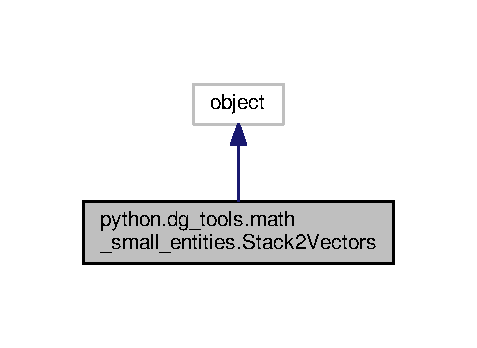
\includegraphics[width=229pt]{classpython_1_1dg__tools_1_1math__small__entities_1_1Stack2Vectors__inherit__graph}
\end{center}
\end{figure}


Collaboration diagram for python.\+dg\+\_\+tools.\+math\+\_\+small\+\_\+entities.\+Stack2\+Vectors\+:
\nopagebreak
\begin{figure}[H]
\begin{center}
\leavevmode
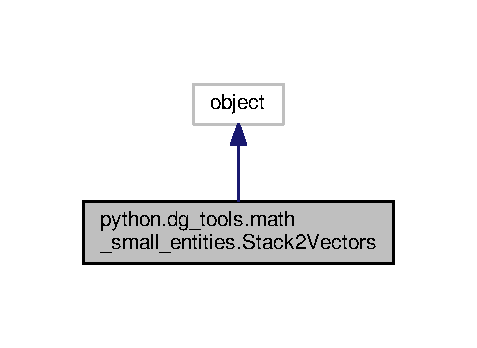
\includegraphics[width=229pt]{classpython_1_1dg__tools_1_1math__small__entities_1_1Stack2Vectors__coll__graph}
\end{center}
\end{figure}
\subsection*{Public Member Functions}
\begin{DoxyCompactItemize}
\item 
def {\bfseries \+\_\+\+\_\+init\+\_\+\+\_\+} (self, sin1, sin2, size1, size2, entity\+\_\+name=\char`\"{}\char`\"{})\hypertarget{classpython_1_1dg__tools_1_1math__small__entities_1_1Stack2Vectors_a5082e1981a9de6406aa09129bee0b347}{}\label{classpython_1_1dg__tools_1_1math__small__entities_1_1Stack2Vectors_a5082e1981a9de6406aa09129bee0b347}

\end{DoxyCompactItemize}
\subsection*{Public Attributes}
\begin{DoxyCompactItemize}
\item 
{\bfseries op}\hypertarget{classpython_1_1dg__tools_1_1math__small__entities_1_1Stack2Vectors_aee9133206d4944bf94d2be498aaa2c7e}{}\label{classpython_1_1dg__tools_1_1math__small__entities_1_1Stack2Vectors_aee9133206d4944bf94d2be498aaa2c7e}

\item 
{\bfseries sin1}\hypertarget{classpython_1_1dg__tools_1_1math__small__entities_1_1Stack2Vectors_ab524298b794cbd1f5d8b239bda6f717c}{}\label{classpython_1_1dg__tools_1_1math__small__entities_1_1Stack2Vectors_ab524298b794cbd1f5d8b239bda6f717c}

\item 
{\bfseries sin2}\hypertarget{classpython_1_1dg__tools_1_1math__small__entities_1_1Stack2Vectors_aeac6844b2c195cfc85d5a2368d491e21}{}\label{classpython_1_1dg__tools_1_1math__small__entities_1_1Stack2Vectors_aeac6844b2c195cfc85d5a2368d491e21}

\item 
{\bfseries sout}\hypertarget{classpython_1_1dg__tools_1_1math__small__entities_1_1Stack2Vectors_a3a20ad03d0a52ffac73e11e8b786253b}{}\label{classpython_1_1dg__tools_1_1math__small__entities_1_1Stack2Vectors_a3a20ad03d0a52ffac73e11e8b786253b}

\end{DoxyCompactItemize}


\subsection{Detailed Description}
Define an easier interface to simple stack 2 vectors. 

The documentation for this class was generated from the following file\+:\begin{DoxyCompactItemize}
\item 
python/dg\+\_\+tools/math\+\_\+small\+\_\+entities.\+py\end{DoxyCompactItemize}

\hypertarget{classpython_1_1dg__tools_1_1math__small__entities_1_1StackZero}{}\section{python.\+dg\+\_\+tools.\+math\+\_\+small\+\_\+entities.\+Stack\+Zero Class Reference}
\label{classpython_1_1dg__tools_1_1math__small__entities_1_1StackZero}\index{python.\+dg\+\_\+tools.\+math\+\_\+small\+\_\+entities.\+Stack\+Zero@{python.\+dg\+\_\+tools.\+math\+\_\+small\+\_\+entities.\+Stack\+Zero}}


Inheritance diagram for python.\+dg\+\_\+tools.\+math\+\_\+small\+\_\+entities.\+Stack\+Zero\+:
\nopagebreak
\begin{figure}[H]
\begin{center}
\leavevmode
\includegraphics[width=210pt]{classpython_1_1dg__tools_1_1math__small__entities_1_1StackZero__inherit__graph}
\end{center}
\end{figure}


Collaboration diagram for python.\+dg\+\_\+tools.\+math\+\_\+small\+\_\+entities.\+Stack\+Zero\+:
\nopagebreak
\begin{figure}[H]
\begin{center}
\leavevmode
\includegraphics[width=210pt]{classpython_1_1dg__tools_1_1math__small__entities_1_1StackZero__coll__graph}
\end{center}
\end{figure}
\subsection*{Public Member Functions}
\begin{DoxyCompactItemize}
\item 
def {\bfseries \+\_\+\+\_\+init\+\_\+\+\_\+} (self, nb\+\_\+0, vec\+\_\+size, vec=None, prefix=\textquotesingle{}\textquotesingle{})\hypertarget{classpython_1_1dg__tools_1_1math__small__entities_1_1StackZero_aeb0f7d55cd51fdf91bca4a05c8457d8b}{}\label{classpython_1_1dg__tools_1_1math__small__entities_1_1StackZero_aeb0f7d55cd51fdf91bca4a05c8457d8b}

\end{DoxyCompactItemize}
\subsection*{Public Attributes}
\begin{DoxyCompactItemize}
\item 
{\bfseries zero}\hypertarget{classpython_1_1dg__tools_1_1math__small__entities_1_1StackZero_afd77c3ead9b408cd92e28918c11a9430}{}\label{classpython_1_1dg__tools_1_1math__small__entities_1_1StackZero_afd77c3ead9b408cd92e28918c11a9430}

\item 
{\bfseries op}\hypertarget{classpython_1_1dg__tools_1_1math__small__entities_1_1StackZero_a0578f0f7b3b6767c71f1c6c64567bd93}{}\label{classpython_1_1dg__tools_1_1math__small__entities_1_1StackZero_a0578f0f7b3b6767c71f1c6c64567bd93}

\item 
{\bfseries sin}\hypertarget{classpython_1_1dg__tools_1_1math__small__entities_1_1StackZero_aeb83d2bb60478305de080dd215560dee}{}\label{classpython_1_1dg__tools_1_1math__small__entities_1_1StackZero_aeb83d2bb60478305de080dd215560dee}

\item 
{\bfseries sout}\hypertarget{classpython_1_1dg__tools_1_1math__small__entities_1_1StackZero_af808bd0b6e64b8aeba17cc160f29484b}{}\label{classpython_1_1dg__tools_1_1math__small__entities_1_1StackZero_af808bd0b6e64b8aeba17cc160f29484b}

\end{DoxyCompactItemize}


The documentation for this class was generated from the following file\+:\begin{DoxyCompactItemize}
\item 
python/dg\+\_\+tools/math\+\_\+small\+\_\+entities.\+py\end{DoxyCompactItemize}

\hypertarget{classdg__tools_1_1Upsampler}{}\section{dg\+\_\+tools\+:\+:Upsampler Class Reference}
\label{classdg__tools_1_1Upsampler}\index{dg\+\_\+tools\+::\+Upsampler@{dg\+\_\+tools\+::\+Upsampler}}


Upsamples the input data by holding the last value for a number of timesteps.  




{\ttfamily \#include $<$upsampler.\+hpp$>$}



Inheritance diagram for dg\+\_\+tools\+:\+:Upsampler\+:
\nopagebreak
\begin{figure}[H]
\begin{center}
\leavevmode
\includegraphics[width=187pt]{classdg__tools_1_1Upsampler__inherit__graph}
\end{center}
\end{figure}


Collaboration diagram for dg\+\_\+tools\+:\+:Upsampler\+:
\nopagebreak
\begin{figure}[H]
\begin{center}
\leavevmode
\includegraphics[width=187pt]{classdg__tools_1_1Upsampler__coll__graph}
\end{center}
\end{figure}
\subsection*{Public Member Functions}
\begin{DoxyCompactItemize}
\item 
{\bfseries Upsampler} (const std\+::string \&name)\hypertarget{classdg__tools_1_1Upsampler_a34ed837b2a5e74ac438b1dabddc694cb}{}\label{classdg__tools_1_1Upsampler_a34ed837b2a5e74ac438b1dabddc694cb}

\item 
void {\bfseries init} (const int \&upsampling\+\_\+factor)\hypertarget{classdg__tools_1_1Upsampler_a5464f7f3d43870ffae21e6fc3ca14bb0}{}\label{classdg__tools_1_1Upsampler_a5464f7f3d43870ffae21e6fc3ca14bb0}

\item 
virtual const std\+::string \& {\bfseries get\+Class\+Name} (void) const \hypertarget{classdg__tools_1_1Upsampler_ac6a7577ec4ad2d1692c238b04655f644}{}\label{classdg__tools_1_1Upsampler_ac6a7577ec4ad2d1692c238b04655f644}

\item 
dg\+::\+Vector \& {\bfseries data\+\_\+out\+\_\+callback} (dg\+::\+Vector \&history, int time)\hypertarget{classdg__tools_1_1Upsampler_a8136079012a13ec172f1084bc147a5b7}{}\label{classdg__tools_1_1Upsampler_a8136079012a13ec172f1084bc147a5b7}

\end{DoxyCompactItemize}
\subsection*{Public Attributes}
\begin{DoxyCompactItemize}
\item 
dg\+::\+Signal\+Ptr$<$ dg\+::\+Vector, int $>$ {\bfseries data\+\_\+input\+S\+IN}\hypertarget{classdg__tools_1_1Upsampler_a52151bf7e4b2c60e290f7954b73aa2d4}{}\label{classdg__tools_1_1Upsampler_a52151bf7e4b2c60e290f7954b73aa2d4}

\item 
dg\+::\+Signal\+Time\+Dependent$<$ dg\+::\+Vector, int $>$ {\bfseries data\+\_\+out\+S\+O\+UT}\hypertarget{classdg__tools_1_1Upsampler_ac24d33450123b89763b6f22ee8432df8}{}\label{classdg__tools_1_1Upsampler_ac24d33450123b89763b6f22ee8432df8}

\end{DoxyCompactItemize}
\subsection*{Static Public Attributes}
\begin{DoxyCompactItemize}
\item 
static const std\+::string {\bfseries C\+L\+A\+S\+S\+\_\+\+N\+A\+ME}\hypertarget{classdg__tools_1_1Upsampler_ae8457eb186d7a4366014c98513982c65}{}\label{classdg__tools_1_1Upsampler_ae8457eb186d7a4366014c98513982c65}

\end{DoxyCompactItemize}
\subsection*{Private Attributes}
\begin{DoxyCompactItemize}
\item 
bool {\bfseries is\+\_\+initialized\+\_\+}\hypertarget{classdg__tools_1_1Upsampler_a083755393f8f65c571ecfbcd14a268a2}{}\label{classdg__tools_1_1Upsampler_a083755393f8f65c571ecfbcd14a268a2}

\item 
int {\bfseries upsampling\+\_\+factor\+\_\+}\hypertarget{classdg__tools_1_1Upsampler_a398d113b1b385ee0f8d702c859511b64}{}\label{classdg__tools_1_1Upsampler_a398d113b1b385ee0f8d702c859511b64}

\item 
int {\bfseries first\+\_\+time\+\_\+}\hypertarget{classdg__tools_1_1Upsampler_a78d524bb8e514007cdf75f1dbff67469}{}\label{classdg__tools_1_1Upsampler_a78d524bb8e514007cdf75f1dbff67469}

\item 
dg\+::\+Vector {\bfseries last\+\_\+input\+\_\+}\hypertarget{classdg__tools_1_1Upsampler_aa54f6ee308bfae9dd26740927319fa4b}{}\label{classdg__tools_1_1Upsampler_aa54f6ee308bfae9dd26740927319fa4b}

\end{DoxyCompactItemize}


\subsection{Detailed Description}
Upsamples the input data by holding the last value for a number of timesteps. 

Pulls the input signal only when the time signal is a multiplicative of the sampling factor. 

The documentation for this class was generated from the following files\+:\begin{DoxyCompactItemize}
\item 
include/dg\+\_\+tools/data/\hyperlink{upsampler_8hpp}{upsampler.\+hpp}\item 
src/data/upsampler.\+cpp\end{DoxyCompactItemize}

\hypertarget{classdg__tools_1_1VectorIntegrator}{}\section{dg\+\_\+tools\+:\+:Vector\+Integrator Class Reference}
\label{classdg__tools_1_1VectorIntegrator}\index{dg\+\_\+tools\+::\+Vector\+Integrator@{dg\+\_\+tools\+::\+Vector\+Integrator}}


Given input data, sum up the input data over time.  




{\ttfamily \#include $<$operator.\+hpp$>$}



Inheritance diagram for dg\+\_\+tools\+:\+:Vector\+Integrator\+:
\nopagebreak
\begin{figure}[H]
\begin{center}
\leavevmode
\includegraphics[width=209pt]{classdg__tools_1_1VectorIntegrator__inherit__graph}
\end{center}
\end{figure}


Collaboration diagram for dg\+\_\+tools\+:\+:Vector\+Integrator\+:
\nopagebreak
\begin{figure}[H]
\begin{center}
\leavevmode
\includegraphics[width=209pt]{classdg__tools_1_1VectorIntegrator__coll__graph}
\end{center}
\end{figure}
\subsection*{Public Member Functions}
\begin{DoxyCompactItemize}
\item 
{\bfseries Vector\+Integrator} (const std\+::string \&name)\hypertarget{classdg__tools_1_1VectorIntegrator_a5c5a7948e49ca2f7d8948a3e0a7439f9}{}\label{classdg__tools_1_1VectorIntegrator_a5c5a7948e49ca2f7d8948a3e0a7439f9}

\item 
virtual const std\+::string \& {\bfseries get\+Class\+Name} (void) const \hypertarget{classdg__tools_1_1VectorIntegrator_a55bebcac4a036c6ff5a3d5be426f27f1}{}\label{classdg__tools_1_1VectorIntegrator_a55bebcac4a036c6ff5a3d5be426f27f1}

\item 
dg\+::\+Vector \& {\bfseries data\+\_\+out\+\_\+callback} (dg\+::\+Vector \&out, int time)\hypertarget{classdg__tools_1_1VectorIntegrator_a3cef1ad9ec653e4d63defedffe3c77d8}{}\label{classdg__tools_1_1VectorIntegrator_a3cef1ad9ec653e4d63defedffe3c77d8}

\end{DoxyCompactItemize}
\subsection*{Public Attributes}
\begin{DoxyCompactItemize}
\item 
bool {\bfseries init\+\_\+}\hypertarget{classdg__tools_1_1VectorIntegrator_a8aacd28288e12d92755fa2ce030998e1}{}\label{classdg__tools_1_1VectorIntegrator_a8aacd28288e12d92755fa2ce030998e1}

\item 
dg\+::\+Vector {\bfseries sum\+\_\+}\hypertarget{classdg__tools_1_1VectorIntegrator_a3e03f4e2fbe8d86f0e5aada6974382ef}{}\label{classdg__tools_1_1VectorIntegrator_a3e03f4e2fbe8d86f0e5aada6974382ef}

\item 
dg\+::\+Signal\+Ptr$<$ dg\+::\+Vector, int $>$ {\bfseries data\+\_\+input\+S\+IN}\hypertarget{classdg__tools_1_1VectorIntegrator_a3486ac49f8e7880954a8dfb29c2e5b18}{}\label{classdg__tools_1_1VectorIntegrator_a3486ac49f8e7880954a8dfb29c2e5b18}

\item 
dg\+::\+Signal\+Time\+Dependent$<$ dg\+::\+Vector, int $>$ {\bfseries data\+\_\+out\+S\+O\+UT}\hypertarget{classdg__tools_1_1VectorIntegrator_ae43ece8351fc054437144e0b8369bf88}{}\label{classdg__tools_1_1VectorIntegrator_ae43ece8351fc054437144e0b8369bf88}

\end{DoxyCompactItemize}
\subsection*{Static Public Attributes}
\begin{DoxyCompactItemize}
\item 
static const std\+::string {\bfseries C\+L\+A\+S\+S\+\_\+\+N\+A\+ME}\hypertarget{classdg__tools_1_1VectorIntegrator_ae540c92d86c7203c41480e680fbcd7ae}{}\label{classdg__tools_1_1VectorIntegrator_ae540c92d86c7203c41480e680fbcd7ae}

\end{DoxyCompactItemize}


\subsection{Detailed Description}
Given input data, sum up the input data over time. 

The documentation for this class was generated from the following files\+:\begin{DoxyCompactItemize}
\item 
include/dg\+\_\+tools/operator.\+hpp\item 
src/operator.\+cpp\end{DoxyCompactItemize}

\hypertarget{classpython_1_1dg__tools_1_1utils_1_1VectorSignal}{}\section{python.\+dg\+\_\+tools.\+utils.\+Vector\+Signal Class Reference}
\label{classpython_1_1dg__tools_1_1utils_1_1VectorSignal}\index{python.\+dg\+\_\+tools.\+utils.\+Vector\+Signal@{python.\+dg\+\_\+tools.\+utils.\+Vector\+Signal}}


Inheritance diagram for python.\+dg\+\_\+tools.\+utils.\+Vector\+Signal\+:
\nopagebreak
\begin{figure}[H]
\begin{center}
\leavevmode
\includegraphics[width=218pt]{classpython_1_1dg__tools_1_1utils_1_1VectorSignal__inherit__graph}
\end{center}
\end{figure}


Collaboration diagram for python.\+dg\+\_\+tools.\+utils.\+Vector\+Signal\+:
\nopagebreak
\begin{figure}[H]
\begin{center}
\leavevmode
\includegraphics[width=218pt]{classpython_1_1dg__tools_1_1utils_1_1VectorSignal__coll__graph}
\end{center}
\end{figure}
\subsection*{Public Member Functions}
\begin{DoxyCompactItemize}
\item 
def {\bfseries \+\_\+\+\_\+init\+\_\+\+\_\+} (self, sig, length=None)\hypertarget{classpython_1_1dg__tools_1_1utils_1_1VectorSignal_a6647fc2c2a69d5f05e72d8842204d893}{}\label{classpython_1_1dg__tools_1_1utils_1_1VectorSignal_a6647fc2c2a69d5f05e72d8842204d893}

\item 
def {\bfseries \+\_\+\+\_\+getitem\+\_\+\+\_\+} (self, val)\hypertarget{classpython_1_1dg__tools_1_1utils_1_1VectorSignal_aa96c5cee8cc77d33f5489bd2e9f1646f}{}\label{classpython_1_1dg__tools_1_1utils_1_1VectorSignal_aa96c5cee8cc77d33f5489bd2e9f1646f}

\item 
def {\bfseries concat} (self, other)\hypertarget{classpython_1_1dg__tools_1_1utils_1_1VectorSignal_a9849ef73dd38b47c751f2b0abcd3e1d8}{}\label{classpython_1_1dg__tools_1_1utils_1_1VectorSignal_a9849ef73dd38b47c751f2b0abcd3e1d8}

\end{DoxyCompactItemize}
\subsection*{Public Attributes}
\begin{DoxyCompactItemize}
\item 
{\bfseries length}\hypertarget{classpython_1_1dg__tools_1_1utils_1_1VectorSignal_a2b26ac0cc2a66a9f2172d870befb482c}{}\label{classpython_1_1dg__tools_1_1utils_1_1VectorSignal_a2b26ac0cc2a66a9f2172d870befb482c}

\end{DoxyCompactItemize}
\subsection*{Private Member Functions}
\begin{DoxyCompactItemize}
\item 
def {\bfseries \+\_\+identity} (self, entity\+\_\+name)\hypertarget{classpython_1_1dg__tools_1_1utils_1_1VectorSignal_a6d05ccf615c9640dd444a475f0ec0db3}{}\label{classpython_1_1dg__tools_1_1utils_1_1VectorSignal_a6d05ccf615c9640dd444a475f0ec0db3}

\end{DoxyCompactItemize}
\subsection*{Private Attributes}
\begin{DoxyCompactItemize}
\item 
{\bfseries \+\_\+add}\hypertarget{classpython_1_1dg__tools_1_1utils_1_1VectorSignal_a42059402a4d2713501869eb2e7053678}{}\label{classpython_1_1dg__tools_1_1utils_1_1VectorSignal_a42059402a4d2713501869eb2e7053678}

\item 
{\bfseries \+\_\+sub}\hypertarget{classpython_1_1dg__tools_1_1utils_1_1VectorSignal_a3fcd7d6305415fc5b67985962bcfa0fe}{}\label{classpython_1_1dg__tools_1_1utils_1_1VectorSignal_a3fcd7d6305415fc5b67985962bcfa0fe}

\end{DoxyCompactItemize}


The documentation for this class was generated from the following file\+:\begin{DoxyCompactItemize}
\item 
python/dg\+\_\+tools/utils.\+py\end{DoxyCompactItemize}

\chapter{File Documentation}
\hypertarget{demo__filter_8py}{}\section{demos/demo\+\_\+filter.py File Reference}
\label{demo__filter_8py}\index{demos/demo\+\_\+filter.\+py@{demos/demo\+\_\+filter.\+py}}


Filter entities demos.  


\subsection*{Variables}
\begin{DoxyCompactItemize}
\item 
{\bfseries demo\+\_\+filter.\+my\+\_\+filter} = Butter\+Worth\+Filter(\textquotesingle{}butterworth\+\_\+filter\textquotesingle{})\hypertarget{demo__filter_8py_a130d66591e0d3f2c230e401ad57d7753}{}\label{demo__filter_8py_a130d66591e0d3f2c230e401ad57d7753}

\item 
int {\bfseries demo\+\_\+filter.\+order} = 6\hypertarget{demo__filter_8py_a007c3b94c2acb3026b358c4e81da3763}{}\label{demo__filter_8py_a007c3b94c2acb3026b358c4e81da3763}

\item 
float {\bfseries demo\+\_\+filter.\+fs} = 5000.\+0\hypertarget{demo__filter_8py_abb4ada25dc7ebdd74e682cac80439e67}{}\label{demo__filter_8py_abb4ada25dc7ebdd74e682cac80439e67}

\item 
float {\bfseries demo\+\_\+filter.\+lowcut} = 600.\+0\hypertarget{demo__filter_8py_ac24b881b7471c905f71c9f196725ebd4}{}\label{demo__filter_8py_ac24b881b7471c905f71c9f196725ebd4}

\item 
float {\bfseries demo\+\_\+filter.\+nyq} = 0.\+5\hypertarget{demo__filter_8py_ab4c267d9ccf3243f72c6c3f264075966}{}\label{demo__filter_8py_ab4c267d9ccf3243f72c6c3f264075966}

\item 
{\bfseries demo\+\_\+filter.\+low} = lowcut/nyq\hypertarget{demo__filter_8py_a5a119c0cb13106a064e599ae0c9fe00b}{}\label{demo__filter_8py_a5a119c0cb13106a064e599ae0c9fe00b}

\item 
float {\bfseries demo\+\_\+filter.\+T} = 0.\+05\hypertarget{demo__filter_8py_aa5c70b37322932d7d54631548a1e3988}{}\label{demo__filter_8py_aa5c70b37322932d7d54631548a1e3988}

\item 
{\bfseries demo\+\_\+filter.\+nsamples} = T$\ast$fs\hypertarget{demo__filter_8py_a7eb6e8d71617c76877efff306bf7bd2e}{}\label{demo__filter_8py_a7eb6e8d71617c76877efff306bf7bd2e}

\item 
{\bfseries demo\+\_\+filter.\+t} = np.\+linspace(0, T, nsamples, endpoint=False)\hypertarget{demo__filter_8py_a9f6ccc86f9fc9dbfed893114dc860d92}{}\label{demo__filter_8py_a9f6ccc86f9fc9dbfed893114dc860d92}

\item 
float {\bfseries demo\+\_\+filter.\+a} = 0.\+02\hypertarget{demo__filter_8py_a07989b33548cbef89b9b53fd686a06c1}{}\label{demo__filter_8py_a07989b33548cbef89b9b53fd686a06c1}

\item 
float {\bfseries demo\+\_\+filter.\+f0} = 600.\+0\hypertarget{demo__filter_8py_aa01427541d4ee283edc3405ce298fa68}{}\label{demo__filter_8py_aa01427541d4ee283edc3405ce298fa68}

\item 
float {\bfseries demo\+\_\+filter.\+x} = 0.\+1\hypertarget{demo__filter_8py_af312a135843af595580510f6d3567804}{}\label{demo__filter_8py_af312a135843af595580510f6d3567804}

\item 
{\bfseries demo\+\_\+filter.\+label}\hypertarget{demo__filter_8py_a3eb129483abbf0526a9cbfba8bbf879c}{}\label{demo__filter_8py_a3eb129483abbf0526a9cbfba8bbf879c}

\item 
list {\bfseries demo\+\_\+filter.\+y} = \mbox{[}$\,$\mbox{]}\hypertarget{demo__filter_8py_a590ad45ef4fb6750568f61bfede1fa57}{}\label{demo__filter_8py_a590ad45ef4fb6750568f61bfede1fa57}

\item 
{\bfseries demo\+\_\+filter.\+value}\hypertarget{demo__filter_8py_a71f09cd8aafc9b8b18973261c2379404}{}\label{demo__filter_8py_a71f09cd8aafc9b8b18973261c2379404}

\item 
{\bfseries demo\+\_\+filter.\+linestyles}\hypertarget{demo__filter_8py_a34279607850e3673ac77cf667d385c69}{}\label{demo__filter_8py_a34279607850e3673ac77cf667d385c69}

\item 
{\bfseries demo\+\_\+filter.\+loc}\hypertarget{demo__filter_8py_a7b95c477f6a0fc95372930c26d1eee1b}{}\label{demo__filter_8py_a7b95c477f6a0fc95372930c26d1eee1b}

\end{DoxyCompactItemize}


\subsection{Detailed Description}
Filter entities demos. 

\begin{DoxyCopyright}{Copyright}
Copyright (c) 2017-\/2019, New York University and Max Planck Gesellschaft, License B\+S\+D-\/3-\/\+Clause 
\end{DoxyCopyright}

\hypertarget{ComImpedanceController_8hpp}{}\section{include/dg\+\_\+tools/\+Com\+Impedance\+Control/\+Com\+Impedance\+Controller.hpp File Reference}
\label{ComImpedanceController_8hpp}\index{include/dg\+\_\+tools/\+Com\+Impedance\+Control/\+Com\+Impedance\+Controller.\+hpp@{include/dg\+\_\+tools/\+Com\+Impedance\+Control/\+Com\+Impedance\+Controller.\+hpp}}


impedance controller implementation for C\+OM (used for quadruped)  


{\ttfamily \#include $<$math.\+h$>$}\\*
{\ttfamily \#include $<$dynamic-\/graph/linear-\/algebra.\+h$>$}\\*
{\ttfamily \#include $<$eigen-\/quadprog/\+Quad\+Prog.\+h$>$}\\*
{\ttfamily \#include $<$dynamic-\/graph/signal-\/time-\/dependent.\+h$>$}\\*
{\ttfamily \#include $<$dynamic-\/graph/signal-\/ptr.\+h$>$}\\*
{\ttfamily \#include $<$dynamic-\/graph/entity.\+h$>$}\\*
Include dependency graph for Com\+Impedance\+Controller.\+hpp\+:
\nopagebreak
\begin{figure}[H]
\begin{center}
\leavevmode
\includegraphics[width=350pt]{ComImpedanceController_8hpp__incl}
\end{center}
\end{figure}
\subsection*{Classes}
\begin{DoxyCompactItemize}
\item 
class \hyperlink{classdynamicgraph_1_1sot_1_1ComImpedanceControl}{dynamicgraph\+::sot\+::\+Com\+Impedance\+Control}
\end{DoxyCompactItemize}


\subsection{Detailed Description}
impedance controller implementation for C\+OM (used for quadruped) 

\begin{DoxyAuthor}{Author}
Avadesh Meduri 
\end{DoxyAuthor}
\begin{DoxyRefDesc}{License}
\item[\hyperlink{license__license000001}{License}]License B\+S\+D-\/3-\/\+Clause \end{DoxyRefDesc}
\begin{DoxyCopyright}{Copyright}
Copyright (c) 2019, New York University and Max Planck Gesellschaft. 
\end{DoxyCopyright}
\begin{DoxyDate}{Date}
2019-\/03-\/19 
\end{DoxyDate}

\hypertarget{reactive__lqr__controller_8hpp}{}\section{include/dg\+\_\+tools/\+Com\+Impedance\+Control/reactive\+\_\+lqr\+\_\+controller.hpp File Reference}
\label{reactive__lqr__controller_8hpp}\index{include/dg\+\_\+tools/\+Com\+Impedance\+Control/reactive\+\_\+lqr\+\_\+controller.\+hpp@{include/dg\+\_\+tools/\+Com\+Impedance\+Control/reactive\+\_\+lqr\+\_\+controller.\+hpp}}


receding reactive L\+QR implementation for solo. The desired trajectory is obtained from the centroidal momentum controller.  


{\ttfamily \#include $<$math.\+h$>$}\\*
{\ttfamily \#include $<$dynamic-\/graph/linear-\/algebra.\+h$>$}\\*
{\ttfamily \#include $<$dynamic-\/graph/signal-\/time-\/dependent.\+h$>$}\\*
{\ttfamily \#include $<$dynamic-\/graph/signal-\/ptr.\+h$>$}\\*
{\ttfamily \#include $<$dynamic-\/graph/entity.\+h$>$}\\*
Include dependency graph for reactive\+\_\+lqr\+\_\+controller.\+hpp\+:
\nopagebreak
\begin{figure}[H]
\begin{center}
\leavevmode
\includegraphics[width=350pt]{reactive__lqr__controller_8hpp__incl}
\end{center}
\end{figure}
\subsection*{Classes}
\begin{DoxyCompactItemize}
\item 
class \hyperlink{classdynamicgraph_1_1sot_1_1ReactiveLQRController}{dynamicgraph\+::sot\+::\+Reactive\+L\+Q\+R\+Controller}
\end{DoxyCompactItemize}


\subsection{Detailed Description}
receding reactive L\+QR implementation for solo. The desired trajectory is obtained from the centroidal momentum controller. 

\begin{DoxyAuthor}{Author}
Avadesh Meduri 
\end{DoxyAuthor}
\begin{DoxyRefDesc}{License}
\item[\hyperlink{license__license000002}{License}]License B\+S\+D-\/3-\/\+Clause \end{DoxyRefDesc}
\begin{DoxyCopyright}{Copyright}
Copyright (c) 2019, New York University and Max Planck Gesellschaft. 
\end{DoxyCopyright}
\begin{DoxyDate}{Date}
2019-\/04-\/29 
\end{DoxyDate}

\hypertarget{control__pd_8hpp}{}\section{include/dg\+\_\+tools/control/control\+\_\+pd.hpp File Reference}
\label{control__pd_8hpp}\index{include/dg\+\_\+tools/control/control\+\_\+pd.\+hpp@{include/dg\+\_\+tools/control/control\+\_\+pd.\+hpp}}
{\ttfamily \#include $<$dynamic-\/graph/linear-\/algebra.\+h$>$}\\*
{\ttfamily \#include $<$dynamic-\/graph/signal-\/time-\/dependent.\+h$>$}\\*
{\ttfamily \#include $<$dynamic-\/graph/signal-\/ptr.\+h$>$}\\*
{\ttfamily \#include $<$dynamic-\/graph/entity.\+h$>$}\\*
Include dependency graph for control\+\_\+pd.\+hpp\+:
\nopagebreak
\begin{figure}[H]
\begin{center}
\leavevmode
\includegraphics[width=350pt]{control__pd_8hpp__incl}
\end{center}
\end{figure}
\subsection*{Classes}
\begin{DoxyCompactItemize}
\item 
class \hyperlink{classdynamicgraph_1_1sot_1_1PDController}{dynamicgraph\+::sot\+::\+P\+D\+Controller}
\end{DoxyCompactItemize}


\subsection{Detailed Description}
\begin{DoxyAuthor}{Author}
François Bleibel, 

Olivier Stasse, 

Steve Heim 
\end{DoxyAuthor}
\begin{DoxyRefDesc}{License}
\item[\hyperlink{license__license000004}{License}]License B\+S\+D-\/3-\/\+Clause \end{DoxyRefDesc}
\begin{DoxyCopyright}{Copyright}
Copyright (c) 2019, New York University and Max Planck Gesellschaft. 
\end{DoxyCopyright}
\begin{DoxyDate}{Date}
2019-\/08-\/05 
\end{DoxyDate}

\hypertarget{upsampler_8hpp}{}\section{include/dg\+\_\+tools/data/upsampler.hpp File Reference}
\label{upsampler_8hpp}\index{include/dg\+\_\+tools/data/upsampler.\+hpp@{include/dg\+\_\+tools/data/upsampler.\+hpp}}
{\ttfamily \#include $<$dynamic-\/graph/linear-\/algebra.\+h$>$}\\*
{\ttfamily \#include $<$dynamic-\/graph/signal-\/time-\/dependent.\+h$>$}\\*
{\ttfamily \#include $<$dynamic-\/graph/signal-\/ptr.\+h$>$}\\*
{\ttfamily \#include $<$dynamic-\/graph/entity.\+h$>$}\\*
Include dependency graph for upsampler.\+hpp\+:
\nopagebreak
\begin{figure}[H]
\begin{center}
\leavevmode
\includegraphics[width=350pt]{upsampler_8hpp__incl}
\end{center}
\end{figure}
\subsection*{Classes}
\begin{DoxyCompactItemize}
\item 
class \hyperlink{classdg__tools_1_1Upsampler}{dg\+\_\+tools\+::\+Upsampler}
\begin{DoxyCompactList}\small\item\em Upsamples the input data by holding the last value for a number of timesteps. \end{DoxyCompactList}\end{DoxyCompactItemize}


\subsection{Detailed Description}
\begin{DoxyAuthor}{Author}
Julian Viereck 
\end{DoxyAuthor}
\begin{DoxyRefDesc}{License}
\item[\hyperlink{license__license000005}{License}]License B\+S\+D-\/3-\/\+Clause \end{DoxyRefDesc}
\begin{DoxyCopyright}{Copyright}
Copyright (c) 2019, New York University and Max Planck Gesellschaft. 
\end{DoxyCopyright}
\begin{DoxyDate}{Date}
2019-\/08-\/05
\end{DoxyDate}
\begin{DoxyAuthor}{Author}
Julian Viereck 
\end{DoxyAuthor}
\begin{DoxyRefDesc}{License}
\item[\hyperlink{license__license000006}{License}]License B\+S\+D-\/3-\/\+Clause \end{DoxyRefDesc}
\begin{DoxyCopyright}{Copyright}
Copyright (c) 2019, New York University and Max Planck Gesellschaft. 
\end{DoxyCopyright}
\begin{DoxyDate}{Date}
2019-\/08-\/05
\end{DoxyDate}
\begin{DoxyAuthor}{Author}
Julian Viereck 
\end{DoxyAuthor}
\begin{DoxyRefDesc}{License}
\item[\hyperlink{license__license000007}{License}]License B\+S\+D-\/3-\/\+Clause \end{DoxyRefDesc}
\begin{DoxyCopyright}{Copyright}
Copyright (c) 2019, New York University and Max Planck Gesellschaft. 
\end{DoxyCopyright}
\begin{DoxyDate}{Date}
2019-\/08-\/05
\end{DoxyDate}
\begin{DoxyAuthor}{Author}
Julian Viereck 
\end{DoxyAuthor}
\begin{DoxyRefDesc}{License}
\item[\hyperlink{license__license000008}{License}]License B\+S\+D-\/3-\/\+Clause \end{DoxyRefDesc}
\begin{DoxyCopyright}{Copyright}
Copyright (c) 2019, New York University and Max Planck Gesellschaft. 
\end{DoxyCopyright}
\begin{DoxyDate}{Date}
2019-\/08-\/05 
\end{DoxyDate}

\hypertarget{power__jump_8hpp}{}\section{include/dg\+\_\+tools/test\+\_\+stand\+\_\+control/power\+\_\+jump.hpp File Reference}
\label{power__jump_8hpp}\index{include/dg\+\_\+tools/test\+\_\+stand\+\_\+control/power\+\_\+jump.\+hpp@{include/dg\+\_\+tools/test\+\_\+stand\+\_\+control/power\+\_\+jump.\+hpp}}


This is a controller to achieve power jumps on the teststand.  


{\ttfamily \#include $<$dynamic-\/graph/linear-\/algebra.\+h$>$}\\*
{\ttfamily \#include $<$dynamic-\/graph/signal-\/time-\/dependent.\+h$>$}\\*
{\ttfamily \#include $<$dynamic-\/graph/signal-\/ptr.\+h$>$}\\*
{\ttfamily \#include $<$dynamic-\/graph/entity.\+h$>$}\\*
Include dependency graph for power\+\_\+jump.\+hpp\+:
\nopagebreak
\begin{figure}[H]
\begin{center}
\leavevmode
\includegraphics[width=350pt]{power__jump_8hpp__incl}
\end{center}
\end{figure}
\subsection*{Classes}
\begin{DoxyCompactItemize}
\item 
class \hyperlink{classdynamicgraph_1_1sot_1_1PowerJumpControl}{dynamicgraph\+::sot\+::\+Power\+Jump\+Control}
\end{DoxyCompactItemize}


\subsection{Detailed Description}
This is a controller to achieve power jumps on the teststand. 

\begin{DoxyAuthor}{Author}
Avadesh Meduri 
\end{DoxyAuthor}
\begin{DoxyRefDesc}{License}
\item[\hyperlink{license__license000010}{License}]License B\+S\+D-\/3-\/\+Clause \end{DoxyRefDesc}
\begin{DoxyCopyright}{Copyright}
Copyright (c) 2019, New York University and Max Planck Gesellschaft. 
\end{DoxyCopyright}
\begin{DoxyDate}{Date}
2019-\/04-\/14 
\end{DoxyDate}

\hypertarget{filter_8py}{}\section{python/dg\+\_\+tools/filter.py File Reference}
\label{filter_8py}\index{python/dg\+\_\+tools/filter.\+py@{python/dg\+\_\+tools/filter.\+py}}


Filter entities factory.  


\subsection*{Classes}
\begin{DoxyCompactItemize}
\item 
class \hyperlink{classpython_1_1dg__tools_1_1filter_1_1ButterWorthFilter}{python.\+dg\+\_\+tools.\+filter.\+Butter\+Worth\+Filter}
\begin{DoxyCompactList}\small\item\em Butterworth filter implementation in dynamic graph. \end{DoxyCompactList}\end{DoxyCompactItemize}


\subsection{Detailed Description}
Filter entities factory. 

\begin{DoxyCopyright}{Copyright}
Copyright (c) 2017-\/2019, New York University and Max Planck Gesellschaft, License B\+S\+D-\/3-\/\+Clause 
\end{DoxyCopyright}

\hypertarget{leg__impedance__controller_8py}{}\section{python/dg\+\_\+tools/leg\+\_\+impedance\+\_\+control/leg\+\_\+impedance\+\_\+controller.py File Reference}
\label{leg__impedance__controller_8py}\index{python/dg\+\_\+tools/leg\+\_\+impedance\+\_\+control/leg\+\_\+impedance\+\_\+controller.\+py@{python/dg\+\_\+tools/leg\+\_\+impedance\+\_\+control/leg\+\_\+impedance\+\_\+controller.\+py}}


This code contains implementation of leg impedance impedance\+\_\+controller.  


\subsection*{Classes}
\begin{DoxyCompactItemize}
\item 
class \hyperlink{classpython_1_1dg__tools_1_1leg__impedance__control_1_1leg__impedance__controller_1_1LegImpedanceController}{python.\+dg\+\_\+tools.\+leg\+\_\+impedance\+\_\+control.\+leg\+\_\+impedance\+\_\+controller.\+Leg\+Impedance\+Controller}
\end{DoxyCompactItemize}


\subsection{Detailed Description}
This code contains implementation of leg impedance impedance\+\_\+controller. 

\begin{DoxyAuthor}{Author}
Avadesh Meduri 
\end{DoxyAuthor}
\begin{DoxyRefDesc}{License}
\item[\hyperlink{license__license000013}{License}]License B\+S\+D-\/3-\/\+Clause \end{DoxyRefDesc}
\begin{DoxyCopyright}{Copyright}
Copyright (c) 2019, New York University and Max Planck Gesellschaft. 
\end{DoxyCopyright}
\begin{DoxyDate}{Date}
2019-\/02-\/06 
\end{DoxyDate}

\hypertarget{quad__leg__impedance__controller_8py}{}\section{python/dg\+\_\+tools/leg\+\_\+impedance\+\_\+control/quad\+\_\+leg\+\_\+impedance\+\_\+controller.py File Reference}
\label{quad__leg__impedance__controller_8py}\index{python/dg\+\_\+tools/leg\+\_\+impedance\+\_\+control/quad\+\_\+leg\+\_\+impedance\+\_\+controller.\+py@{python/dg\+\_\+tools/leg\+\_\+impedance\+\_\+control/quad\+\_\+leg\+\_\+impedance\+\_\+controller.\+py}}


Impedance controller implementation on a quadruped.  


\subsection*{Classes}
\begin{DoxyCompactItemize}
\item 
class \hyperlink{classpython_1_1dg__tools_1_1leg__impedance__control_1_1quad__leg__impedance__controller_1_1QuadrupedLegImpedanceController}{python.\+dg\+\_\+tools.\+leg\+\_\+impedance\+\_\+control.\+quad\+\_\+leg\+\_\+impedance\+\_\+controller.\+Quadruped\+Leg\+Impedance\+Controller}
\item 
class \hyperlink{classpython_1_1dg__tools_1_1leg__impedance__control_1_1quad__leg__impedance__controller_1_1QuadrupedComControl}{python.\+dg\+\_\+tools.\+leg\+\_\+impedance\+\_\+control.\+quad\+\_\+leg\+\_\+impedance\+\_\+controller.\+Quadruped\+Com\+Control}
\end{DoxyCompactItemize}


\subsection{Detailed Description}
Impedance controller implementation on a quadruped. 

\begin{DoxyAuthor}{Author}
Avadesh Meduri 
\end{DoxyAuthor}
\begin{DoxyRefDesc}{License}
\item[\hyperlink{license__license000014}{License}]License B\+S\+D-\/3-\/\+Clause \end{DoxyRefDesc}
\begin{DoxyCopyright}{Copyright}
Copyright (c) 2019, New York University and Max Planck Gesellschaft. 
\end{DoxyCopyright}
\begin{DoxyDate}{Date}
2019-\/03-\/01 
\end{DoxyDate}

\hypertarget{solo12__impedance__controller_8py}{}\section{python/dg\+\_\+tools/leg\+\_\+impedance\+\_\+control/solo12\+\_\+impedance\+\_\+controller.py File Reference}
\label{solo12__impedance__controller_8py}\index{python/dg\+\_\+tools/leg\+\_\+impedance\+\_\+control/solo12\+\_\+impedance\+\_\+controller.\+py@{python/dg\+\_\+tools/leg\+\_\+impedance\+\_\+control/solo12\+\_\+impedance\+\_\+controller.\+py}}


Implement leg impedance controller and 4 leg control for solo12.  


\subsection*{Classes}
\begin{DoxyCompactItemize}
\item 
class \hyperlink{classpython_1_1dg__tools_1_1leg__impedance__control_1_1solo12__impedance__controller_1_1Solo12ComController}{python.\+dg\+\_\+tools.\+leg\+\_\+impedance\+\_\+control.\+solo12\+\_\+impedance\+\_\+controller.\+Solo12\+Com\+Controller}
\item 
class \hyperlink{classpython_1_1dg__tools_1_1leg__impedance__control_1_1solo12__impedance__controller_1_1Solo12LegImpedanceController}{python.\+dg\+\_\+tools.\+leg\+\_\+impedance\+\_\+control.\+solo12\+\_\+impedance\+\_\+controller.\+Solo12\+Leg\+Impedance\+Controller}
\begin{DoxyCompactList}\small\item\em Impedance controller for single leg on solo12. \end{DoxyCompactList}\item 
class \hyperlink{classpython_1_1dg__tools_1_1leg__impedance__control_1_1solo12__impedance__controller_1_1Solo12ImpedanceController}{python.\+dg\+\_\+tools.\+leg\+\_\+impedance\+\_\+control.\+solo12\+\_\+impedance\+\_\+controller.\+Solo12\+Impedance\+Controller}
\begin{DoxyCompactList}\small\item\em Implements leg impedance controller for the solo12 robot. \end{DoxyCompactList}\end{DoxyCompactItemize}


\subsection{Detailed Description}
Implement leg impedance controller and 4 leg control for solo12. 

\begin{DoxyAuthor}{Author}
Julian Viereck 

Avadesh Meduri 
\end{DoxyAuthor}
\begin{DoxyRefDesc}{License}
\item[\hyperlink{license__license000015}{License}]License B\+S\+D-\/3-\/\+Clause \end{DoxyRefDesc}
\begin{DoxyCopyright}{Copyright}
Copyright (c) 2019, New York University and Max Planck Gesellschaft. 
\end{DoxyCopyright}
\begin{DoxyDate}{Date}
2019-\/11-\/27 Differences between solo8 and solo12 code\+:
\begin{DoxyItemize}
\item Using 3-\/dim vector to specify desired position and velocity instead of 6-\/dim
\item Use kp and kd value for each leg separately 
\end{DoxyItemize}
\end{DoxyDate}

\hypertarget{traj__generators_8py}{}\section{python/dg\+\_\+tools/traj\+\_\+generators.py File Reference}
\label{traj__generators_8py}\index{python/dg\+\_\+tools/traj\+\_\+generators.\+py@{python/dg\+\_\+tools/traj\+\_\+generators.\+py}}


This code contains different trajectory generation functions.  


\subsection*{Classes}
\begin{DoxyCompactItemize}
\item 
class \hyperlink{classpython_1_1dg__tools_1_1traj__generators_1_1CircularCartesianTrajectoryGenerator}{python.\+dg\+\_\+tools.\+traj\+\_\+generators.\+Circular\+Cartesian\+Trajectory\+Generator}
\begin{DoxyCompactList}\small\item\em generates a circular circular\+\_\+trajectory\+\_\+generator \end{DoxyCompactList}\end{DoxyCompactItemize}
\subsection*{Functions}
\begin{DoxyCompactItemize}
\item 
def {\bfseries python.\+dg\+\_\+tools.\+traj\+\_\+generators.\+sine\+\_\+generator} (amplitude, omega, phase, bias, entity\+Name)\hypertarget{traj__generators_8py_aebaab9631fa96c005c4997394cf69bd8}{}\label{traj__generators_8py_aebaab9631fa96c005c4997394cf69bd8}

\item 
def \hyperlink{traj__generators_8py_a9ce2792fafeec3e1de0d03fff8ac8365}{python.\+dg\+\_\+tools.\+traj\+\_\+generators.\+circular\+\_\+trajectory\+\_\+generator} (radius\+\_\+x, radius\+\_\+z, omega, phase, bias, entity\+Name)\hypertarget{traj__generators_8py_a9ce2792fafeec3e1de0d03fff8ac8365}{}\label{traj__generators_8py_a9ce2792fafeec3e1de0d03fff8ac8365}

\begin{DoxyCompactList}\small\item\em generates a circular circular\+\_\+trajectory\+\_\+generator \end{DoxyCompactList}\item 
def {\bfseries python.\+dg\+\_\+tools.\+traj\+\_\+generators.\+cubic\+\_\+interpolator} (init\+\_\+vector\+\_\+signal, goal\+\_\+vector\+\_\+signal, entity\+Name)\hypertarget{traj__generators_8py_a95bc5b726c7b5a2d1497496888142722}{}\label{traj__generators_8py_a95bc5b726c7b5a2d1497496888142722}

\end{DoxyCompactItemize}
\subsection*{Variables}
\begin{DoxyCompactItemize}
\item 
{\bfseries python.\+dg\+\_\+tools.\+traj\+\_\+generators.\+add\+\_\+pi} = Add\+\_\+of\+\_\+double(\textquotesingle{}pi\textquotesingle{})\hypertarget{traj__generators_8py_a335cd611a3cd7dc967f6b9959a2daa64}{}\label{traj__generators_8py_a335cd611a3cd7dc967f6b9959a2daa64}

\item 
{\bfseries python.\+dg\+\_\+tools.\+traj\+\_\+generators.\+value}\hypertarget{traj__generators_8py_a71c7a6d3a4ff3f2d4a03673c5b8f65c6}{}\label{traj__generators_8py_a71c7a6d3a4ff3f2d4a03673c5b8f65c6}

\item 
{\bfseries python.\+dg\+\_\+tools.\+traj\+\_\+generators.\+pi} = add\+\_\+pi.\+sout\hypertarget{traj__generators_8py_a2e2264c95807ae69c2699b4901b8e9fb}{}\label{traj__generators_8py_a2e2264c95807ae69c2699b4901b8e9fb}

\end{DoxyCompactItemize}


\subsection{Detailed Description}
This code contains different trajectory generation functions. 

\begin{DoxyAuthor}{Author}
Avadesh Meduri 
\end{DoxyAuthor}
\begin{DoxyRefDesc}{License}
\item[\hyperlink{license__license000018}{License}]License B\+S\+D-\/3-\/\+Clause \end{DoxyRefDesc}
\begin{DoxyCopyright}{Copyright}
Copyright (c) 2019, New York University and Max Planck Gesellschaft. 
\end{DoxyCopyright}
\begin{DoxyDate}{Date}
2019-\/02-\/06 
\end{DoxyDate}

%--- End generated contents ---

% Index
\backmatter
\newpage
\phantomsection
\clearemptydoublepage
\addcontentsline{toc}{chapter}{Index}
\printindex

\end{document}
